\section{The fit model}

The search described in chapter \ref{chp:VLQ} and the one described in this chapter share a similar fit model; the few existing differences are highlighted in this section. A total of nine search regions are used in the fit, summarised in table \ref{sec:tth:tab:reg} along with the corresponding final discriminating variable used: the classification BDT in signal regions and $H_{\rm T}^{\rm had}$, defined as the scalar sum of jet $\pt$, in the control regions.
\begin{table}\footnotesize
\begin{center}
\begin{tabular}{|c|c|c|c|}
  \hline \hline
    & 4 jets & 5 jets & $\ge$6jets \\
  \hline
  2 b-tagged jets & $H_{\rm T}^{\rm had}$ & $H_{\rm T}^{\rm had}$ & $H_{\rm T}^{\rm had}$\\
  \hline
  3 b-tagged jets & $H_{\rm T}^{\rm had}$ & $H_{\rm T}^{\rm had}$ & $BDT_{6j3b}$\\
  \hline
  $\ge$4 b-tagged jets&$H_{\rm T}^{\rm had}$&$BDT_{5j4b}$&$BDT_{6j4b}$\\
 \hline \hline
\end{tabular}
\captionsetup{width=0.85\textwidth}  \caption{\small Summary of regions included in the fit and variable used in each region. The subscript in the BDT output variables indicates that a specific BDT is trained in each region.}
\label{sec:tth:tab:reg}
\end{center}
\end{table}
\par Control regions have a very low sensitivity to signal, and so $H_{\rm T}^{\rm had}$  is chosen due to its sensitivity to the background modelling and to systematic uncertainties such
as jet energy scale or $b$-tagging, which have a $\pt$ dependence. No explicit validation regions are considered, but the agreement for other kinematic distributions not used in the fit is used to gain confidence in the overall procedure. The control regions have high data statistics and the fit of $H_{\rm T}^{\rm had}$  allows controlling the impact of systematic uncertainties primarily affecting the $t\bar{t}$+light-jets background; it also provides more sensitivity to systematic uncertainties affecting the $t\bar{t}+\ge1c$ background compared to the search described in chapter \ref{chp:VLQ}. The following sections provide a summary of the differences in the treatment of systematic uncertainties compared to that in section \ref{chp:vlq:sec:syst}, as well as a discussion of the results obtained from the fit to data.


\subsection{Systematic uncertainties}
\label{sec:tth:systunc}

\subsubsection[$t\bar{t}$ modelling]{\boldmath{$t\bar{t}$} modelling}
Due to the presence of high-statistics regions with different jet multiplicity in the fit, the uncertainty on the modelling of the $\pt$ of the $t\bar{t}$ system is included. The $\pt$ of the $t\bar{t}$ system is directly linked to the emission of additional jets. The uncertainty is evaluated by taking the full difference between applying and not applying the reweighting to match the NNLO prediction on the \pt of the $\ttbar$ system.\par
The increased sensitivity to $t\bar{t}+\ge1c$ events gives the possibility to measure the normalisation of this background directly from data. Therefore a free-floating parameter is used in the fit instead of the $50\%$ normalisation uncertainty. The increased sensitivity to the $t\bar{t}+\ge1c$ background also calls for a more complete treatment of systematic uncertainties for this background component. Therefore, the difference between the NLO sample described in section \ref{sec:data:ttc}, and an inclusive $t\bar{t}$ sample produced with {\sc MG5$\_$aMC} is taken as an uncertainty on the $t\bar{t}+\ge1c$  prediction.

\subsubsection[$W/Z$+jets modelling]{\boldmath{$V$}+jets modelling}
The uncertainties affecting the normalisation of the $V$+jets background are estimated separately for $W$+jets and $Z$+jets. For $W$+jets a normalisation uncertainty of $30\%$ is assumed, taken to be uncorrelated across jet multiplicity. An additional $30\%$ normalisation uncertainty is assumed for $W+$HF-jets correlated between $W+\ge1c$  and $W+\ge1b$ processes but uncorrelated across $b$-tag multiplicity. Therefore, a total of six independent nuisance parameters are considered.
For $Z$+jets, which has a smaller contribution to the total background, a normalisation uncertainty of $30\%$ is assumed, considered as one nuisance parameter. No additional uncertainty on $Z$+HF-jets is assumed.

\subsubsection{Single-top-quark modelling}
Since in the search regions the event kinematics  is not as extreme as for the $T\bar{T}/t\bar{t}t\bar{t}$ search, there is enough MC statistics to evaluate the uncertainties for $Wt$-channel production described in section \ref{sec:data:singletop} in each region, without summing in quadrature with those for the $t$-channel and $s$-channel processes. Therefore, a total of five independent nuisance parameters are considered in the fit.

\subsubsection[$t\bar{t}+V$ modelling uncertainties]{\boldmath{$t\bar{t}+V$} modelling}

The uncertainty on the $t\bar{t}Z$ and $t\bar{t}W$ normalisations is $15\%$, from the uncertainties on their respective NLO theoretical cross sections. This uncertainty is treated as uncorrelated between $t\bar{t}Z$ and $t\bar{t}W$ and is split into scale and PDF uncertainties, also treated as uncorrelated. Therefore, a total of four independent nuisance parameters are considered.

\subsubsection{Multijet modelling}

A $50\%$ normalisation uncertainty is taken as correlated across jet multiplicity but uncorrelated across lepton flavours (electron or muon) and $b$-tag multiplicity. Thus, a total of six independent nuisance parameters are considered.

\subsubsection{Signal modelling}
The uncertainty on the $t\bar{t}H$ signal cross section is $+10\%/-13\%$, including contributions from scale and PDF uncertainties, which are treated as uncorrelated \cite{ttH1,ttH4,Yu:2014cka}. Uncertainties on the Higgs-boson branching ratios are also considered; these amount to $2.2\%$ for the $b\bar{b}$ decay mode \cite{hdecay}. An additional uncertainty on the choice of parton shower and hadronisation model is derived by comparing the default prediction from {\sc MG5$\_$aMC+Pythia8} to that from {\sc MG5$\_$aMC}+{\sc Herwig++}. Finally, the effect of the QCD scale choice is evaluated by varying the renormalisation and factorisation scales up and down by a factor of two. Therefore, a total of seven independent nuisance parameters are considered.


\subsection{Fit results}

A fit to the data is performed in the nine analysis channels under the signal-plus-background hypothesis. The resulting fitted NPs and the corresponding correlation matrix can be found in figures \ref{sec:ttH:fig:Fit} and \ref{sec:ttH:fig:matr} respectively.


\begin{figure}[htbp!]
\begin{subfigure}{0.5\textwidth}
  \centering
  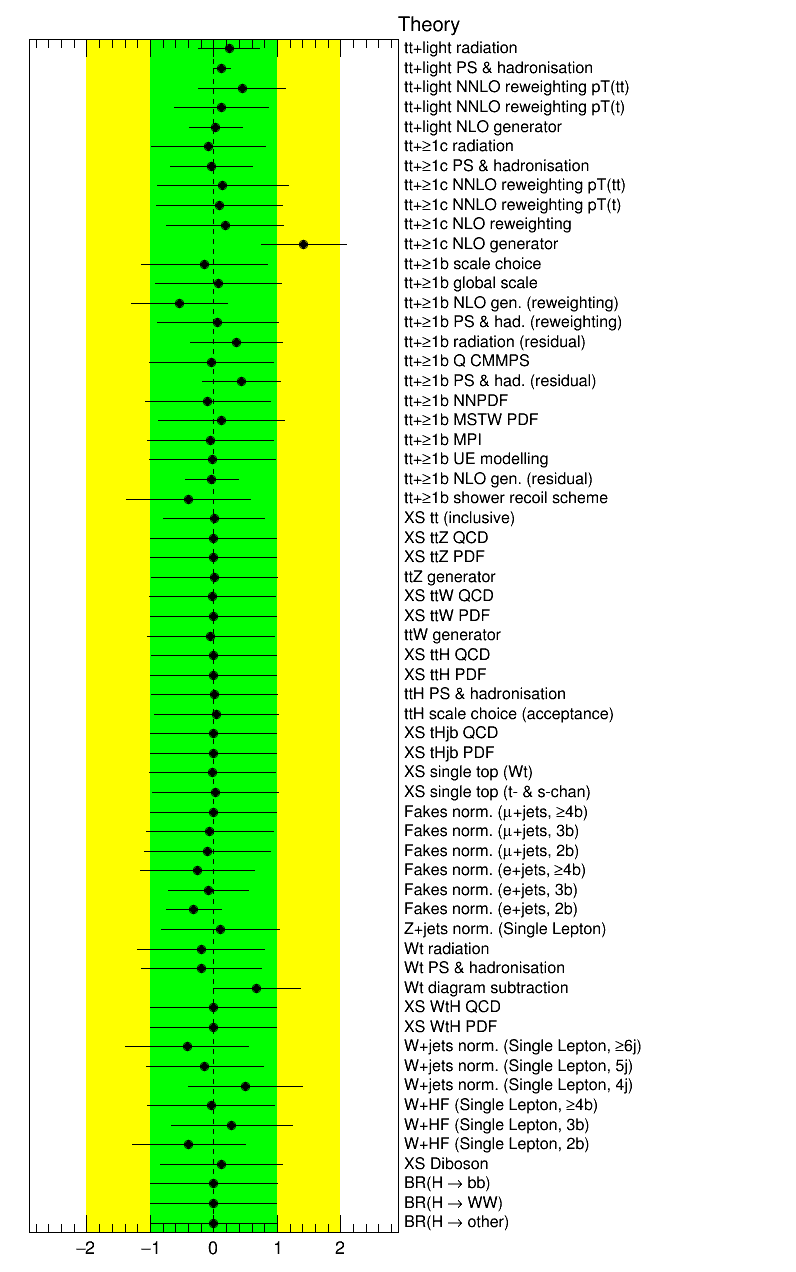
\includegraphics[width=0.9\textwidth]{figures/ttH/NuisPar_Theory.png}
\end{subfigure}
\begin{subfigure}{0.5\textwidth}
  \centering
  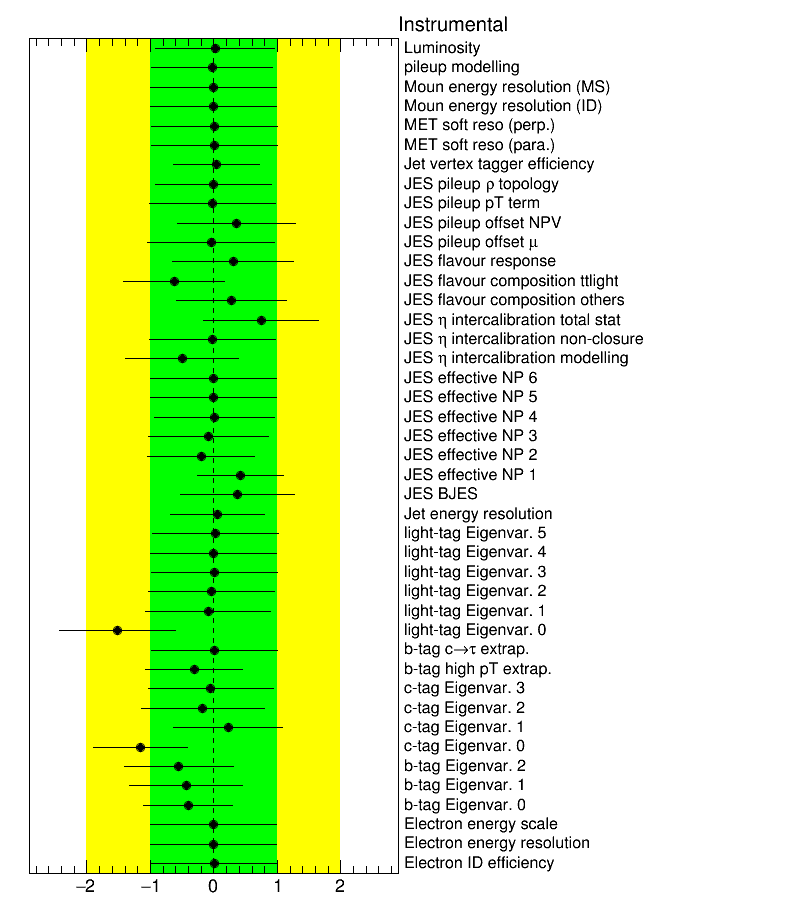
\includegraphics[width=0.9\textwidth]{figures/ttH/NuisPar_Instrumental.png}
\end{subfigure}
\captionsetup{width=0.85\textwidth}  \caption{\small Nuisance parameters from the fit to data in the single-lepton channel under the signal-plus-background hypothesis. A detailed description of the naming of the NPs can be found in appendix \ref{App:Glossary}.}
\label{sec:ttH:fig:Fit}
\end{figure}

\begin{figure}[h!]
 \centering
 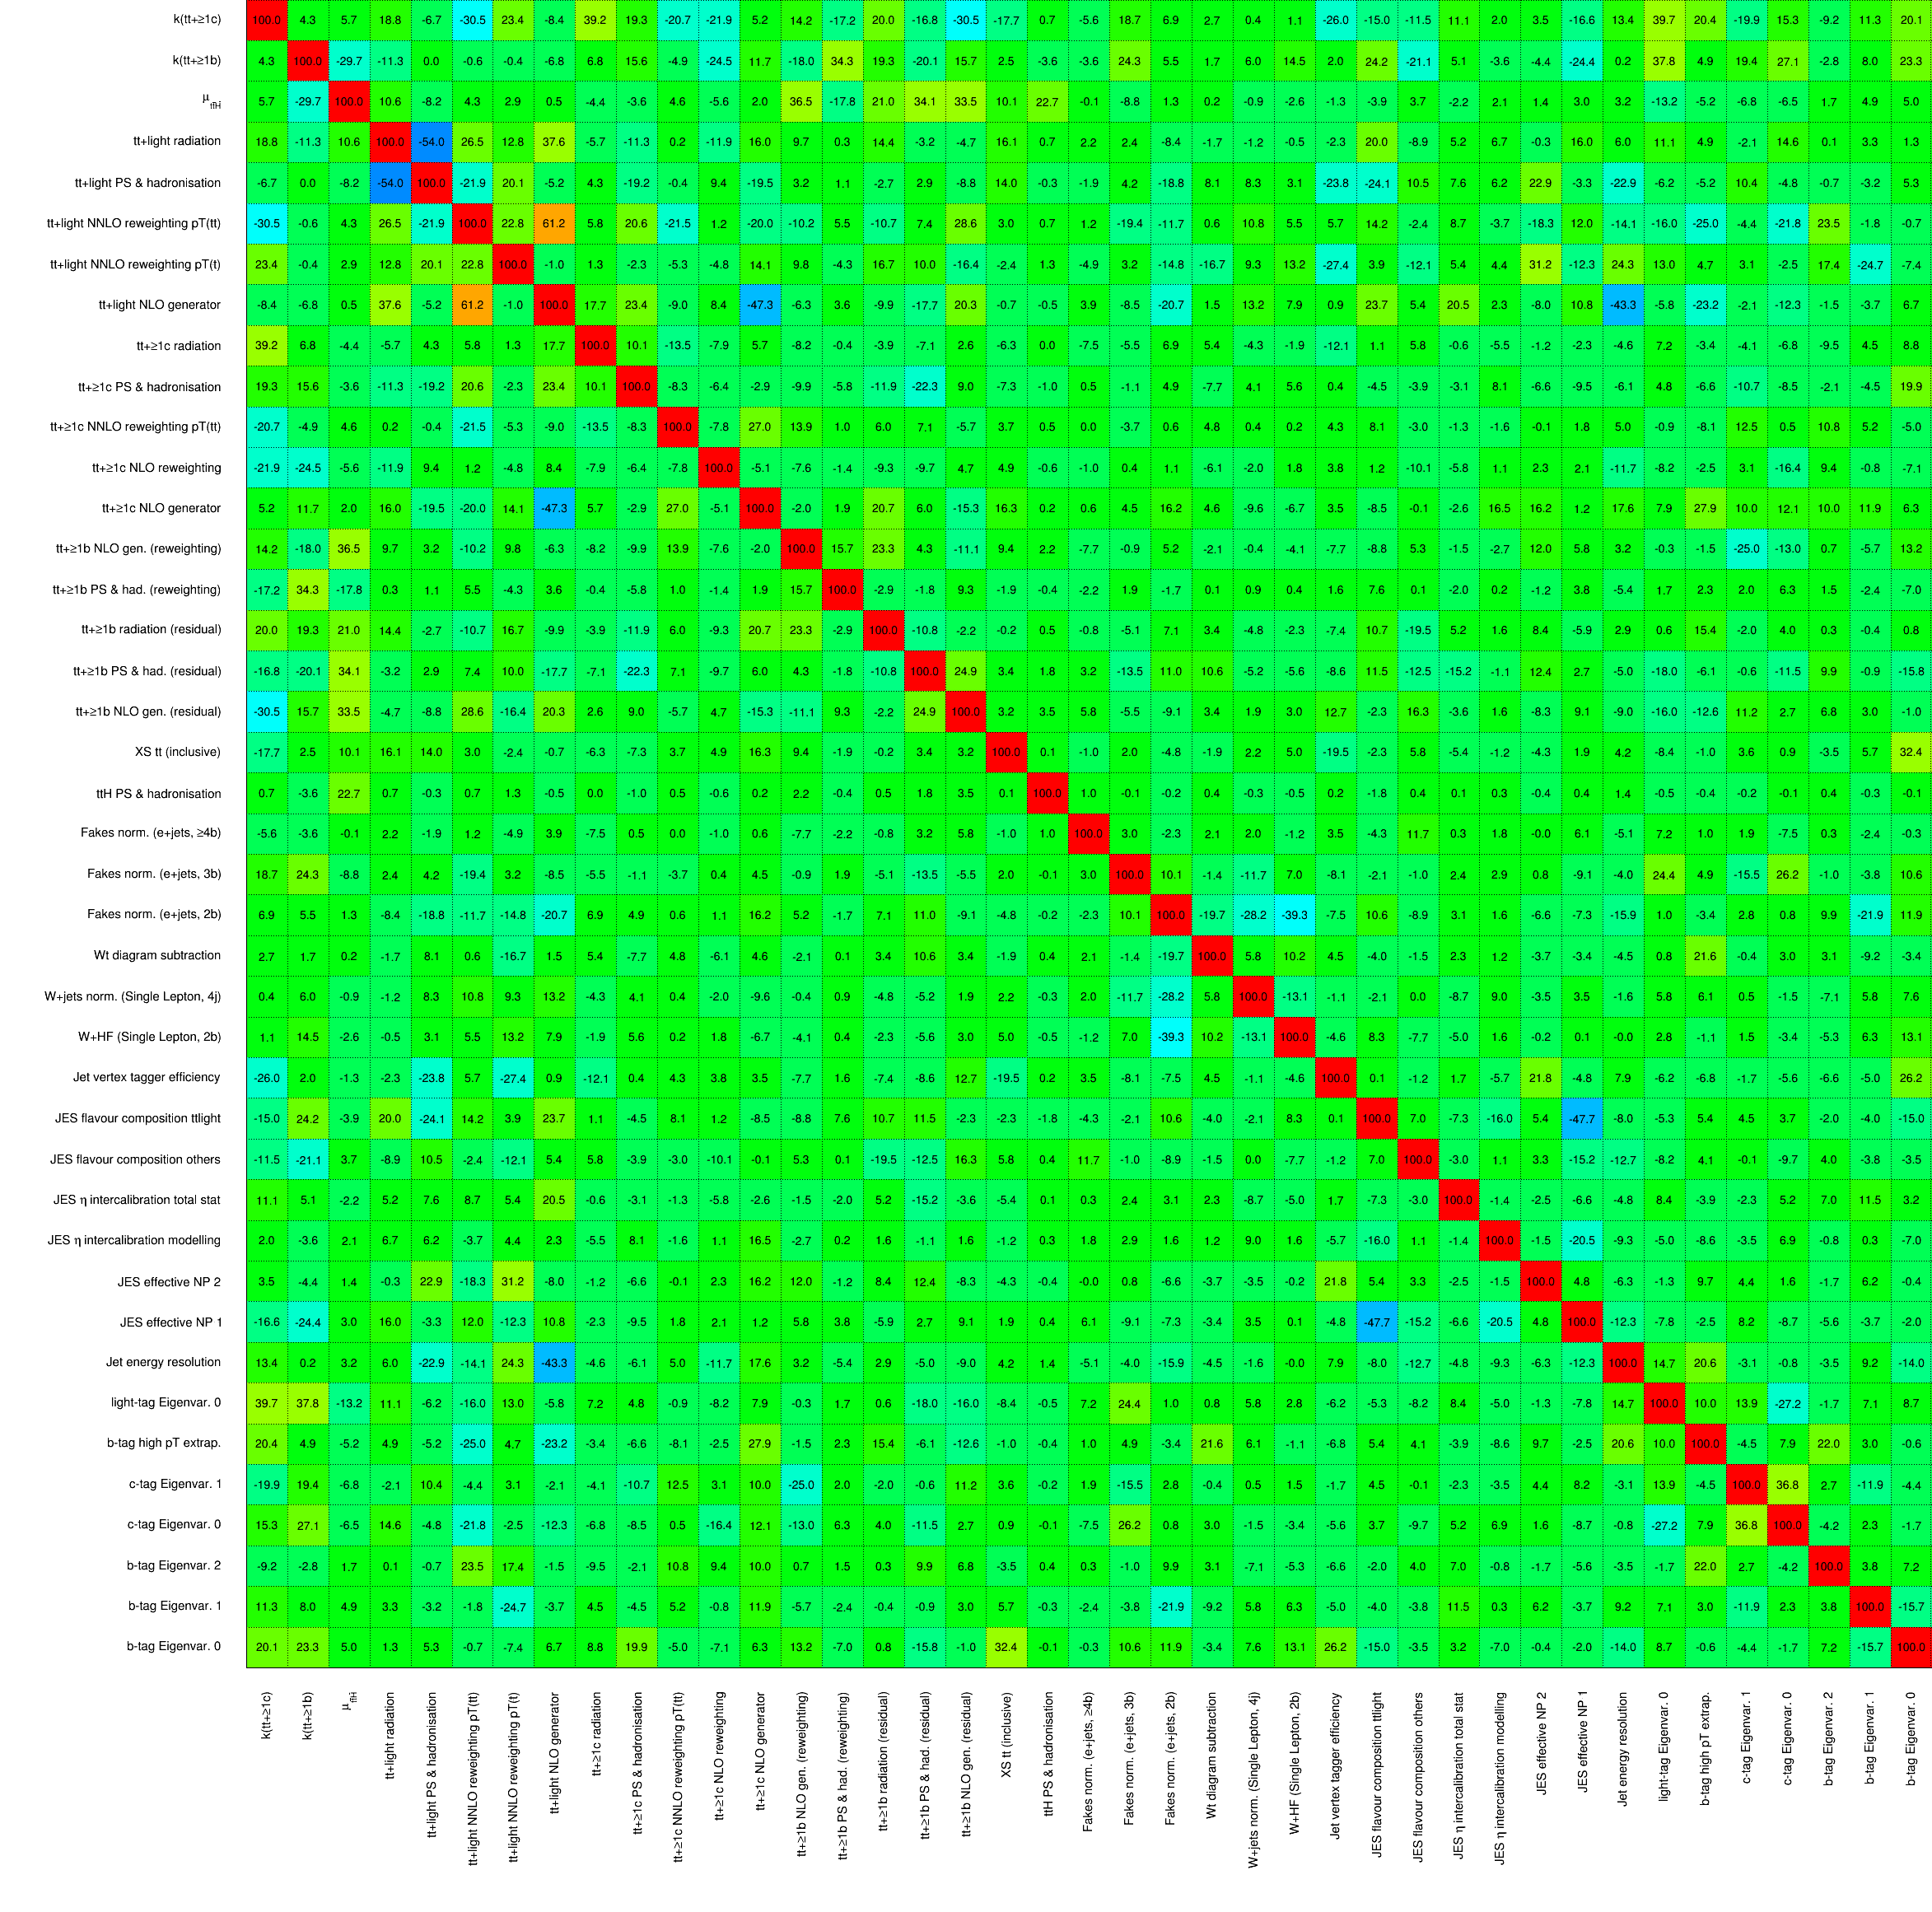
\includegraphics[width=0.5\textwidth]{figures/ttH/CorrMatrix.png}
\captionsetup{width=0.85\textwidth}  \caption{\small Correlation matrix between NPs corresponding to the fit to data in the single-lepton channel under the signal-plus-background hypothesis. Only NPs with a correlation coefficient of at least $20\%$ with any other parameter are displayed.}
\label{sec:ttH:fig:matr}
\end{figure}


The fitted values for the $t\bar{t}+\ge1b$ and $t\bar{t}+\ge1c$ normalisation parameters are $1.2\pm0.2$ and $1.4^{+0.7}_{-0.6}$ respectively.
As discussed in section \ref{sec:fit:vlqdatafit}, given the regions considered in the fit, only few NPs are expected to be pulled and somewhat constrained by the data. Such discussion is also valid for this fit since the dataset and categorisation is very similar. The introduction of the 4-jet and 5-jet channels improves the statistical power of the fit, and some of the pulls and constraints such as the ones that were present in $t\bar{t}+$light-jets modelling or multijet modelling are accentuated. The fit results between the two searches are quite consistent, taking into account the existing differences of fitted regions and uncertainties modelling. \par
A complementary search for $t\bar{t}H (H \to b\bar{b})$ in the dileptonic channel has also been performed in ATLAS \cite{ATLAS-CONF-2016-080}. The analysis procedure in the dileptonic channel is completely equivalent, and given that the datasets are orthogonal, the combination of both analyses can be performed. A combined fit is performed to the nine regions of the single-lepton search and six regions of the dilepton search. The results of the fit are in good agreement between the individual and the combined analyses.\par
Figure \ref{sec:ttH:fig:ranking} demonstrates the effect of various systematic uncertainties on the fitted value of $\mu$ and the constraints provided by the data. The largest effects arises from the modelling of the $t\bar{t}+\ge1b$ background, with six of them being among the ten highest-ranked systematic uncertainties.


\begin{figure}[htb!]
 \centering
 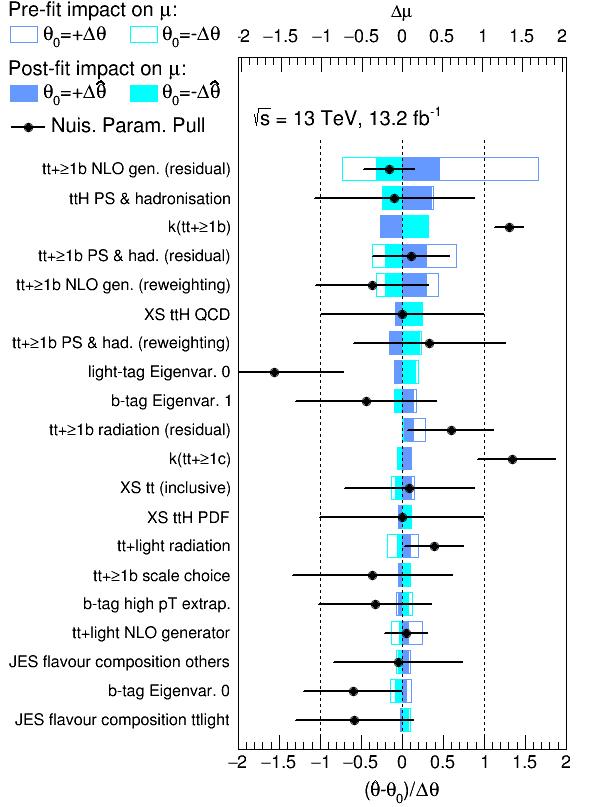
\includegraphics[width=0.5\textwidth]{figures/ttH/Ranking.png}
\captionsetup{width=0.85\textwidth}  \caption{\small The fitted values of the NPs with the largest impact on the measured signal strength. The points, which are drawn conforming to the scale of the bottom axis, show the deviation of each of the fitted NPs, $\hat{\theta}$, from $\theta_{0}$, which is the nominal value of that NP, in units of the pre-fit standard deviation $\Delta\theta$. The error bars show the post-fit uncertainties, $\sigma_{\theta}$, which are close to 1 if the data do not provide any further constraint on that uncertainty. Conversely, a value of $\sigma_{\theta}$ much smaller than 1 indicates a significant reduction with respect to the original uncertainty. The NPs are sorted according to the post-fit effect of each on $\mu$ (plain area) conforming to the scale of the top axis, with those with the largest impact at the top.}
\label{sec:ttH:fig:ranking}
\end{figure}


Figures \ref{sec:tth:fig:hthad1} and \ref{sec:tth:fig:bdt} show the comparison of data and prediction for the $H_{\rm T}^{\rm had}$ and BDT distributions in each of the analysis channels considered before and after the combined fit. The corresponding predicted and observed yields per channel can be found in table \ref{tab:tth:SLyields}, and also displayed in figure \ref{sec:ttH:fig:summary}, before and after the combined fit. Compared to the pre-fit distributions, the total background uncertainty is significantly reduced after the fit, not only in the background-dominated channels, but also in the signal-rich channels, resulting in an increase in the search sensitivity. The reduced uncertainty results from the significant constraints provided by the data on some systematic uncertainties, as well as the anti-correlations among sources of systematic uncertainty resulting from the fit to the data. 

\begin{figure}[htbp!]
\begin{subfigure}{0.24\textwidth}
  \centering
  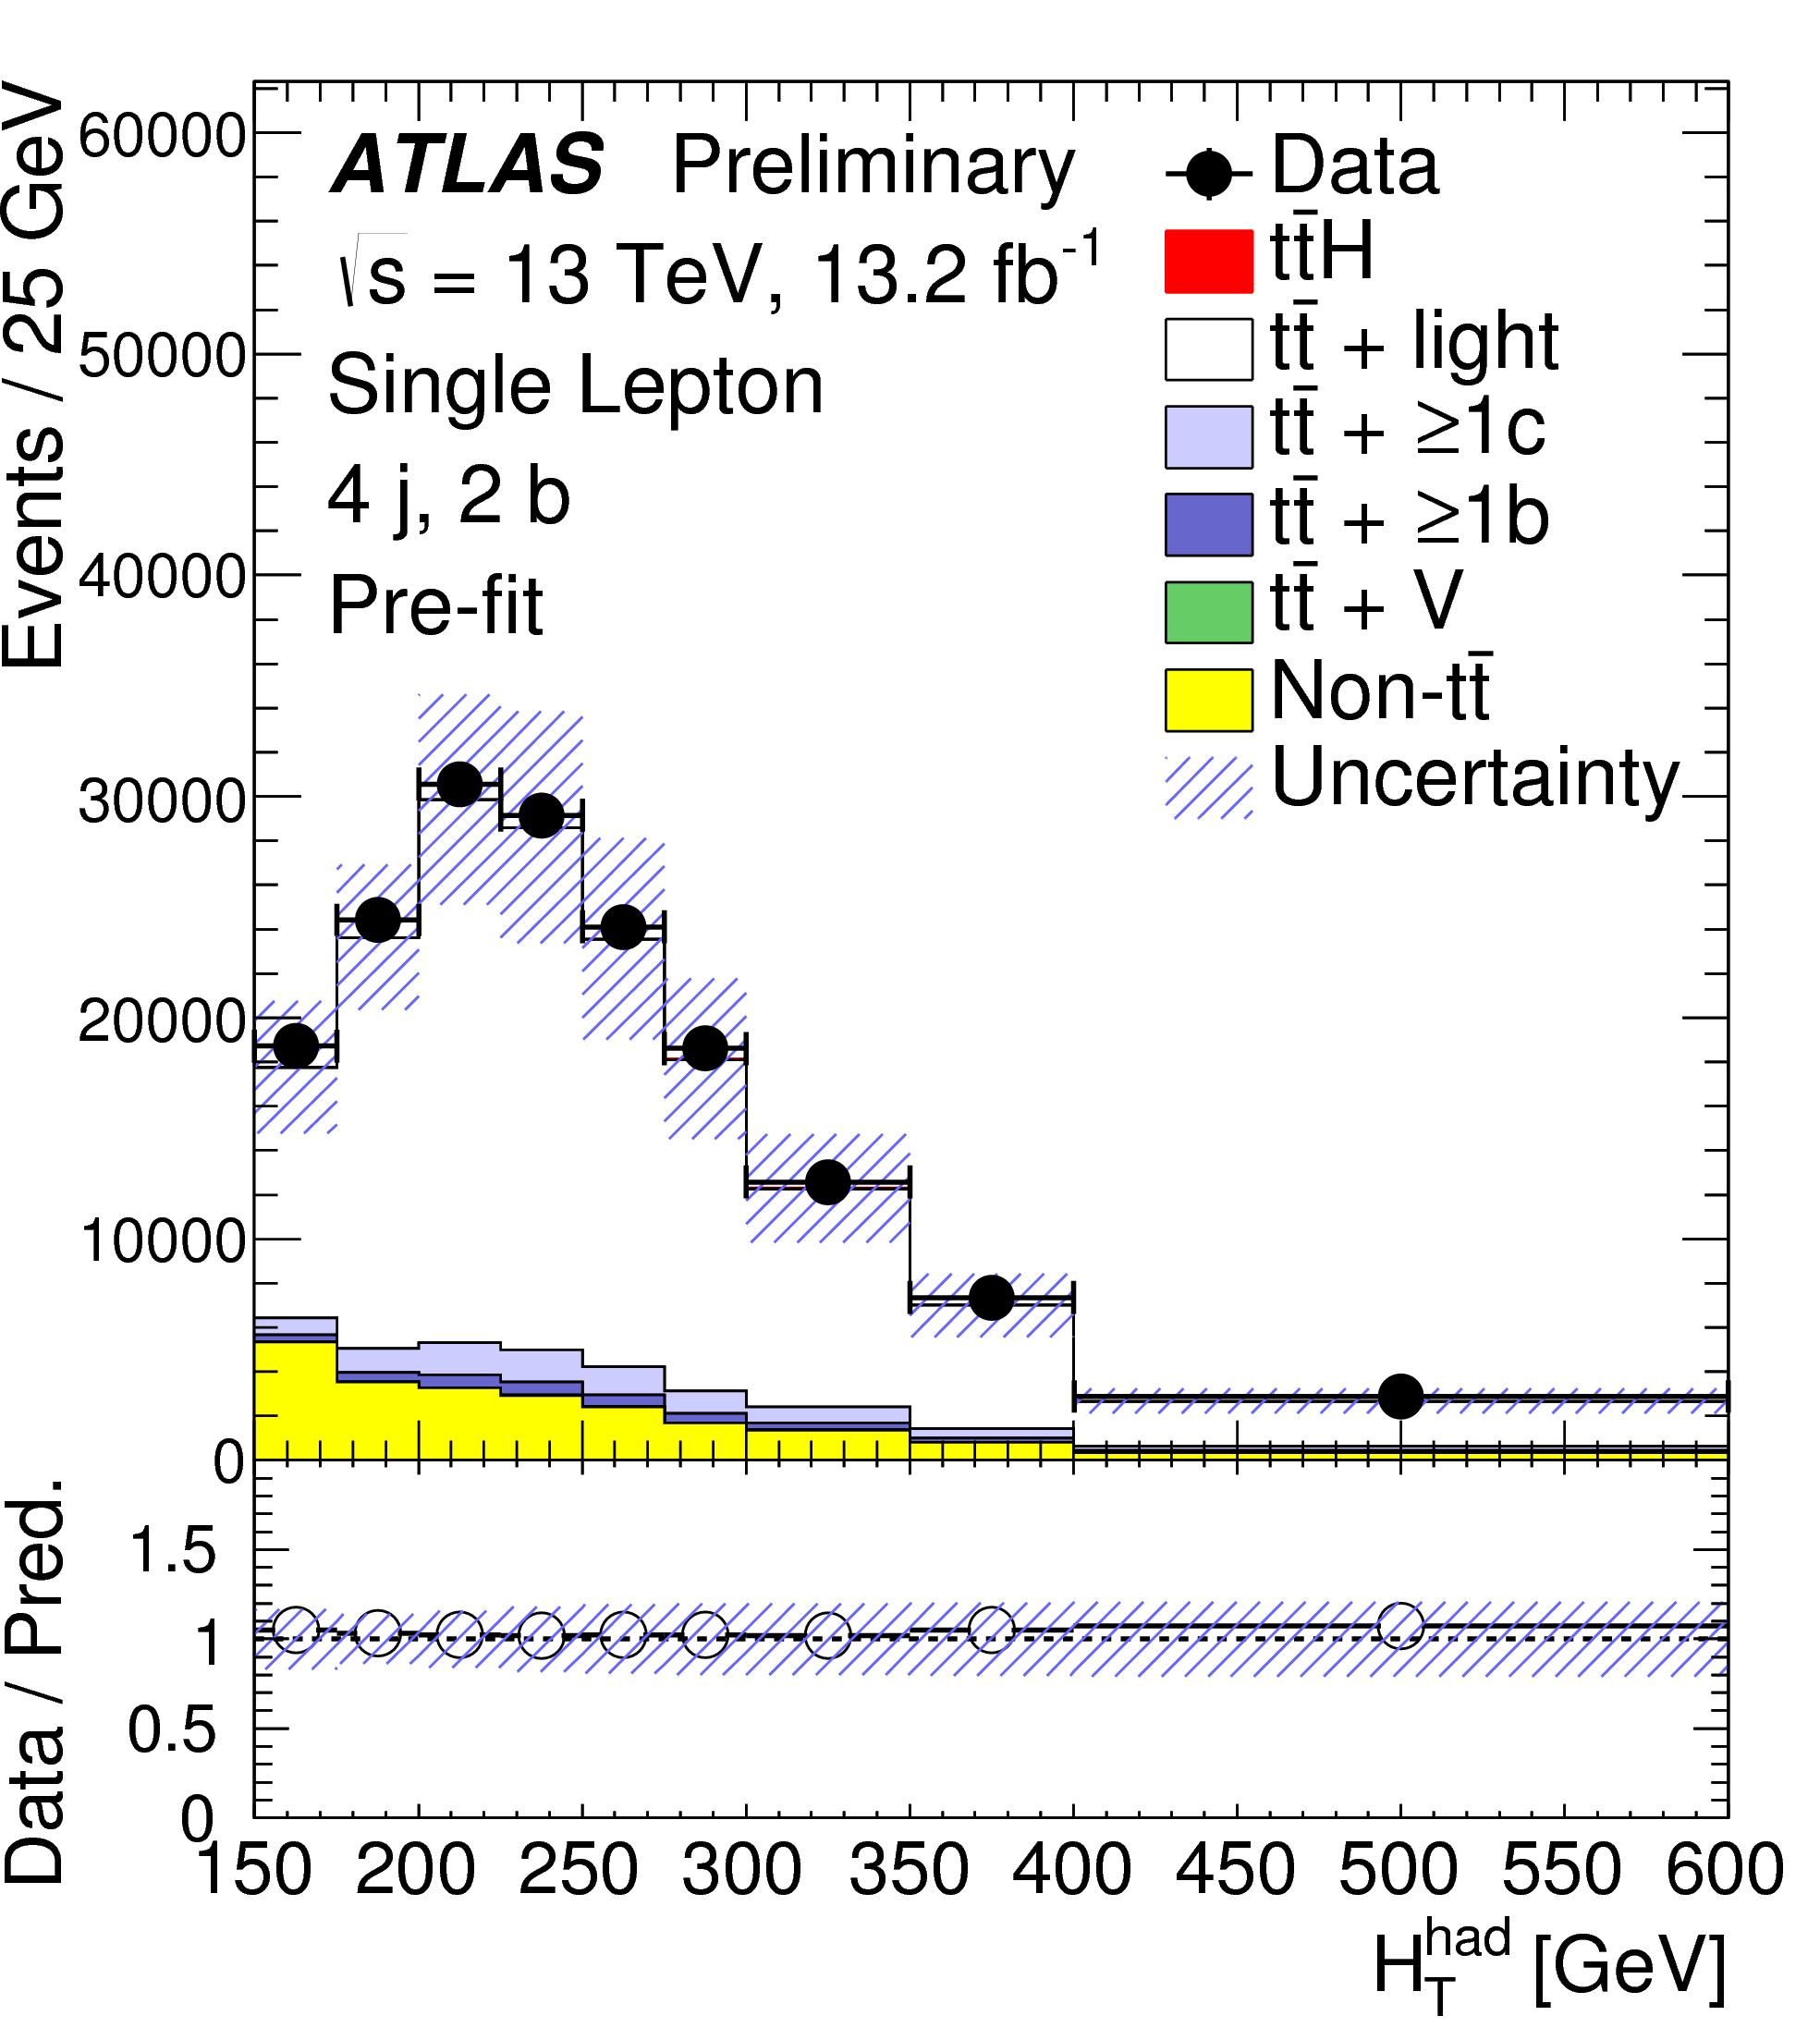
\includegraphics[width=0.9\textwidth]{figures/ttH/fig_07a.png}
  \caption{}
  \label{}
\end{subfigure}
\begin{subfigure}{0.24\textwidth}
  \centering
  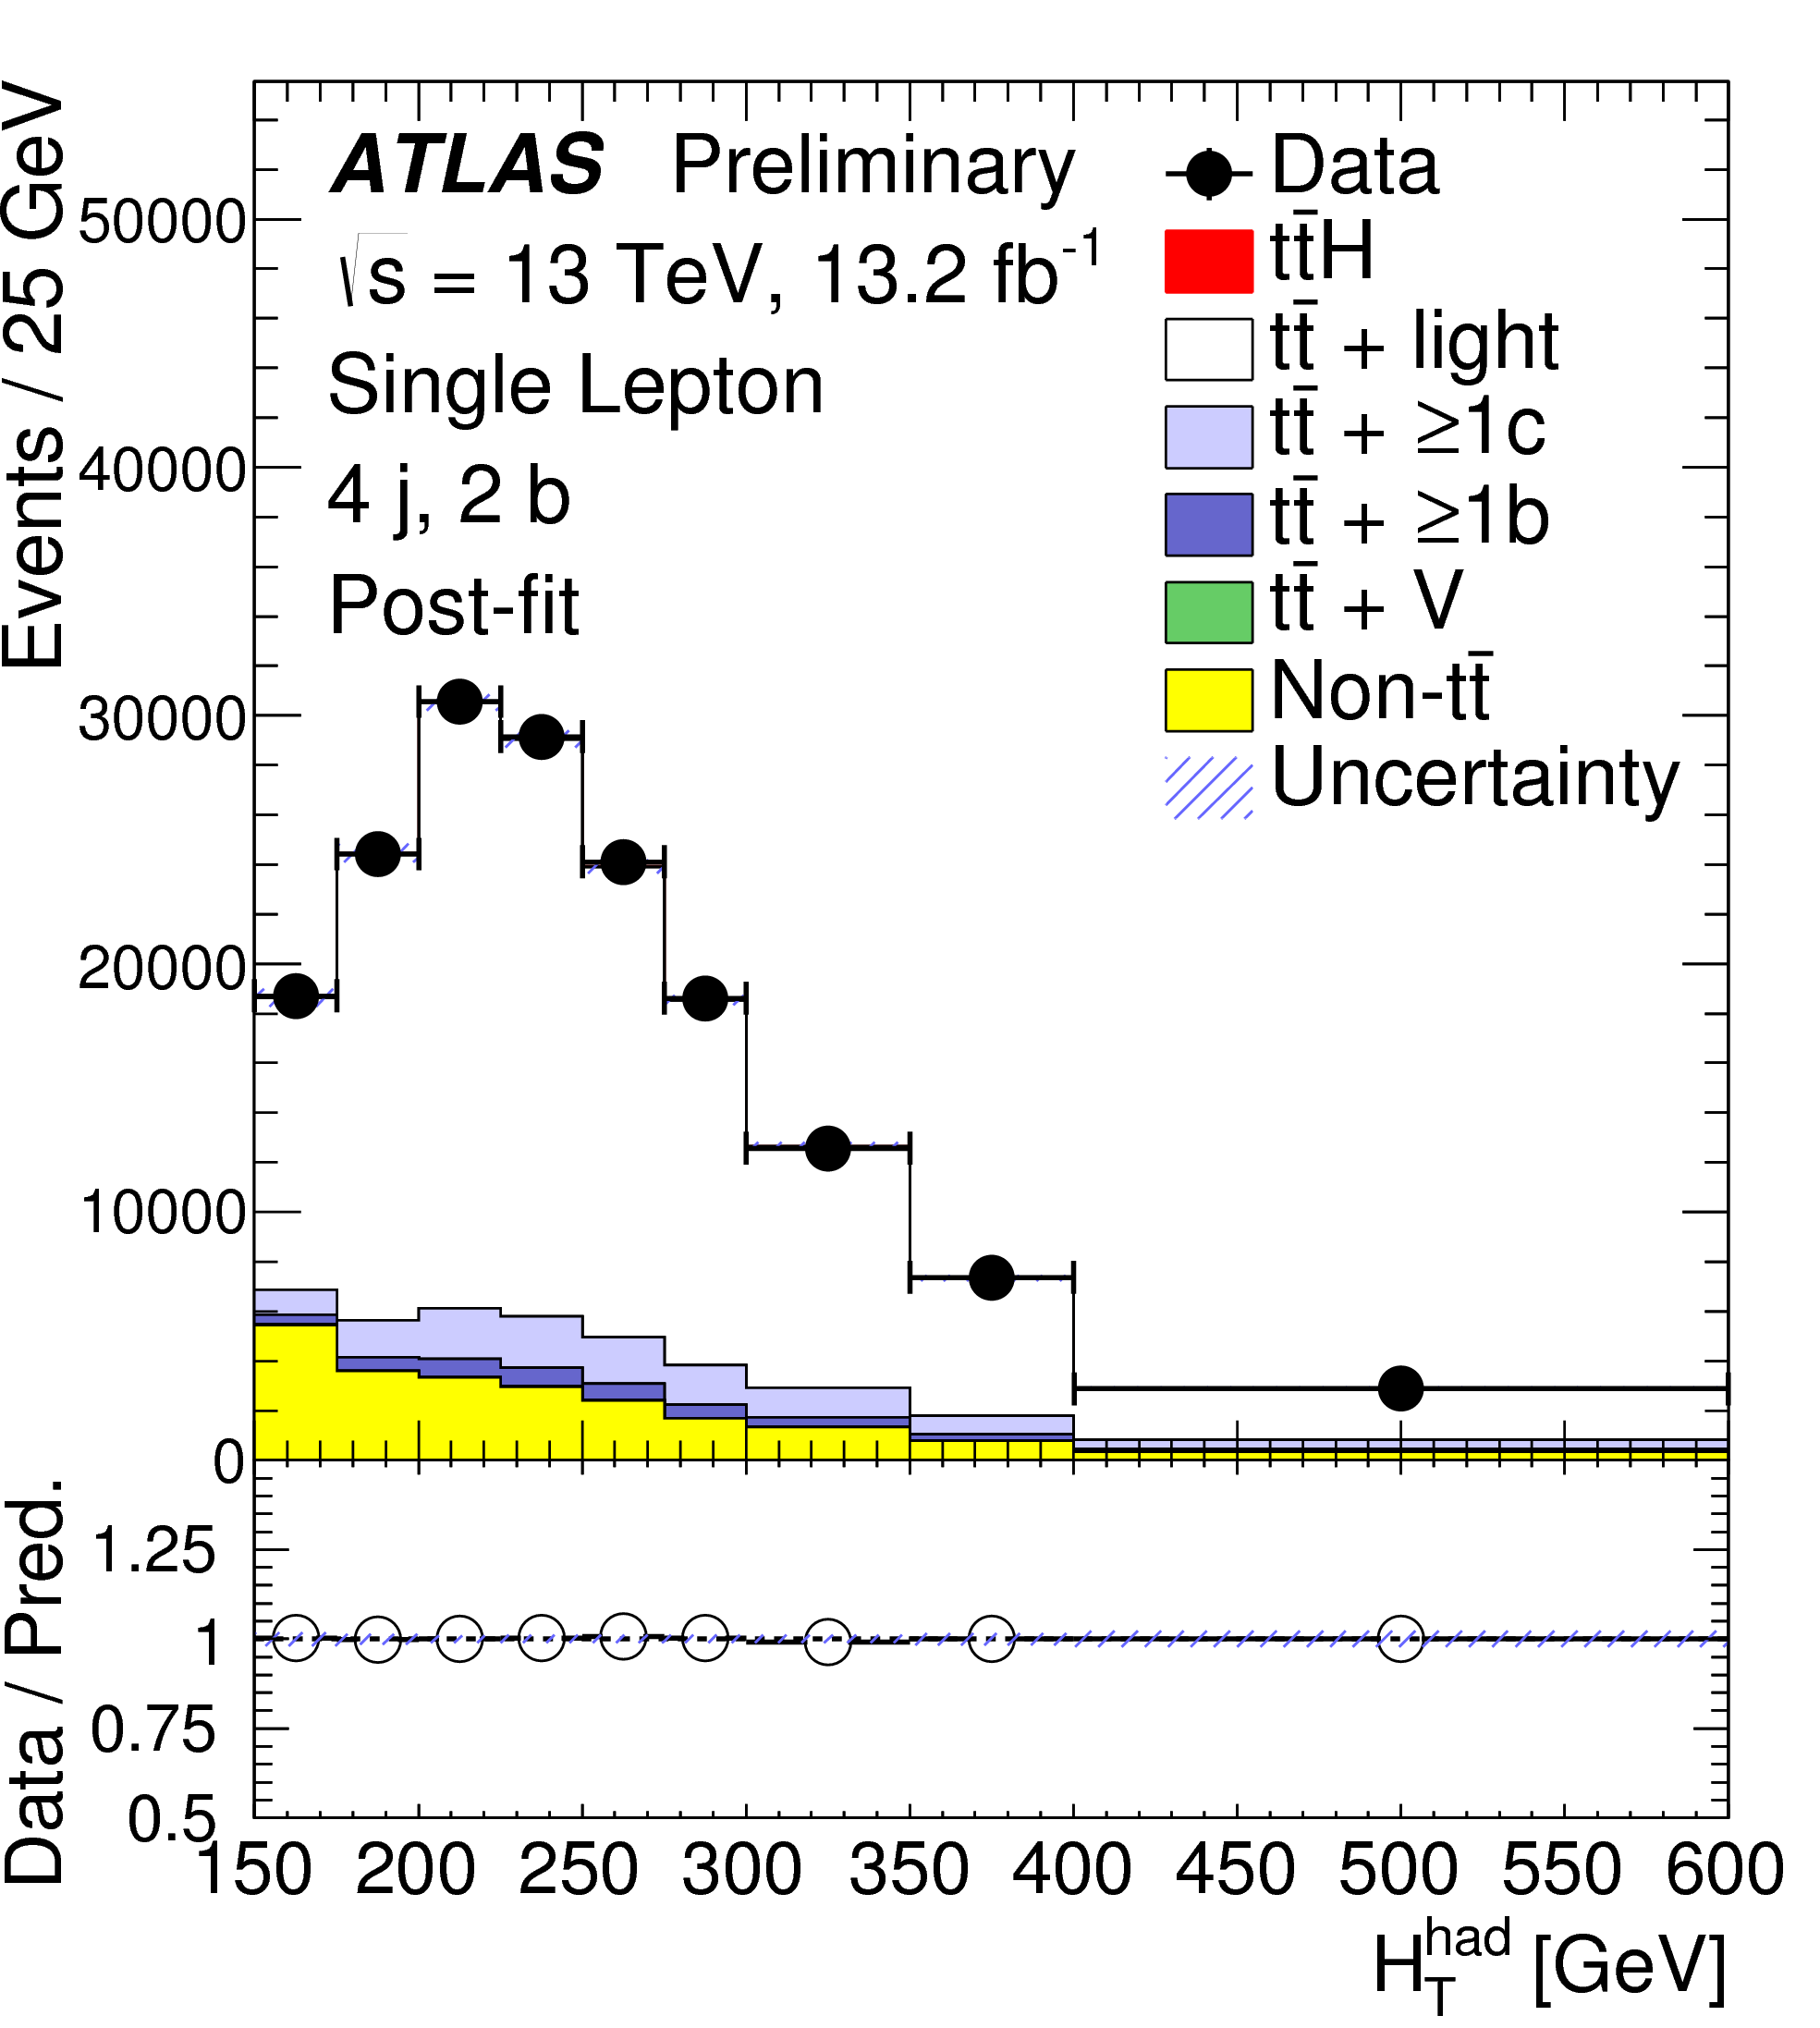
\includegraphics[width=0.9\textwidth]{figures/ttH/fig_07b.png}
  \caption{}
  \label{}
\end{subfigure}
\begin{subfigure}{0.24\textwidth}
  \centering
  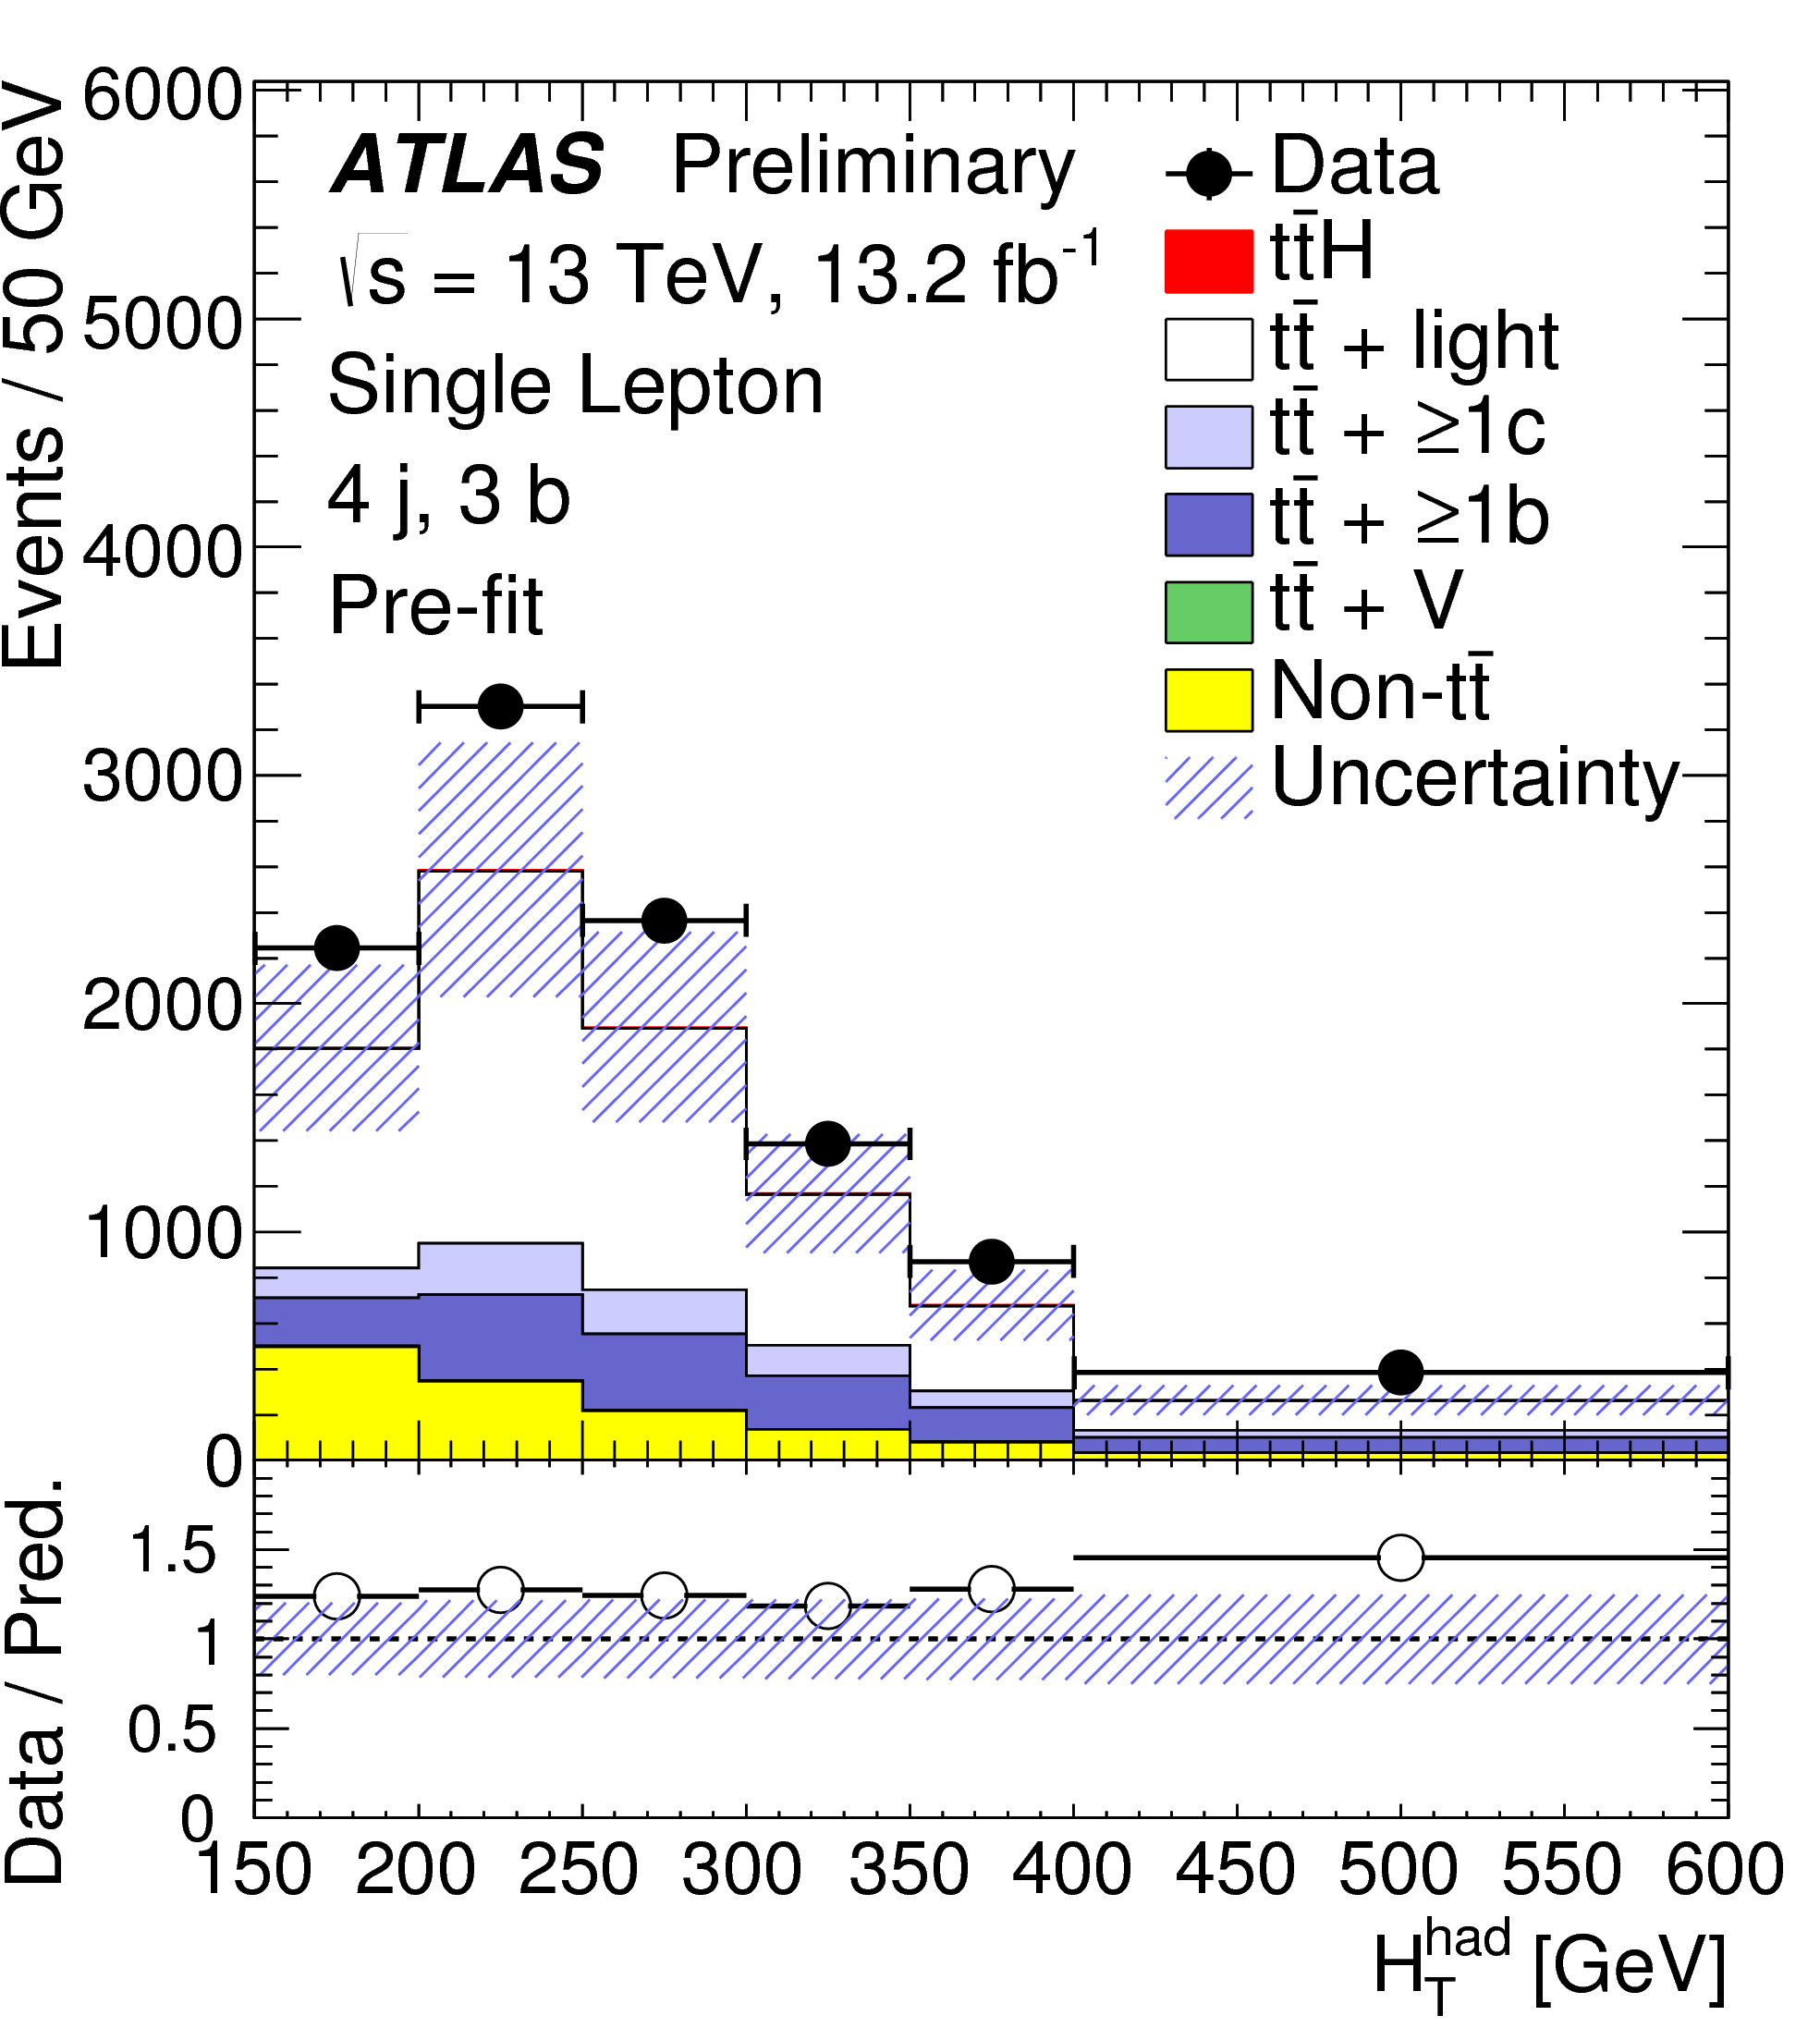
\includegraphics[width=0.9\textwidth]{figures/ttH/fig_07c.png}
  \caption{}
  \label{}
\end{subfigure}
\begin{subfigure}{0.24\textwidth}
  \centering
  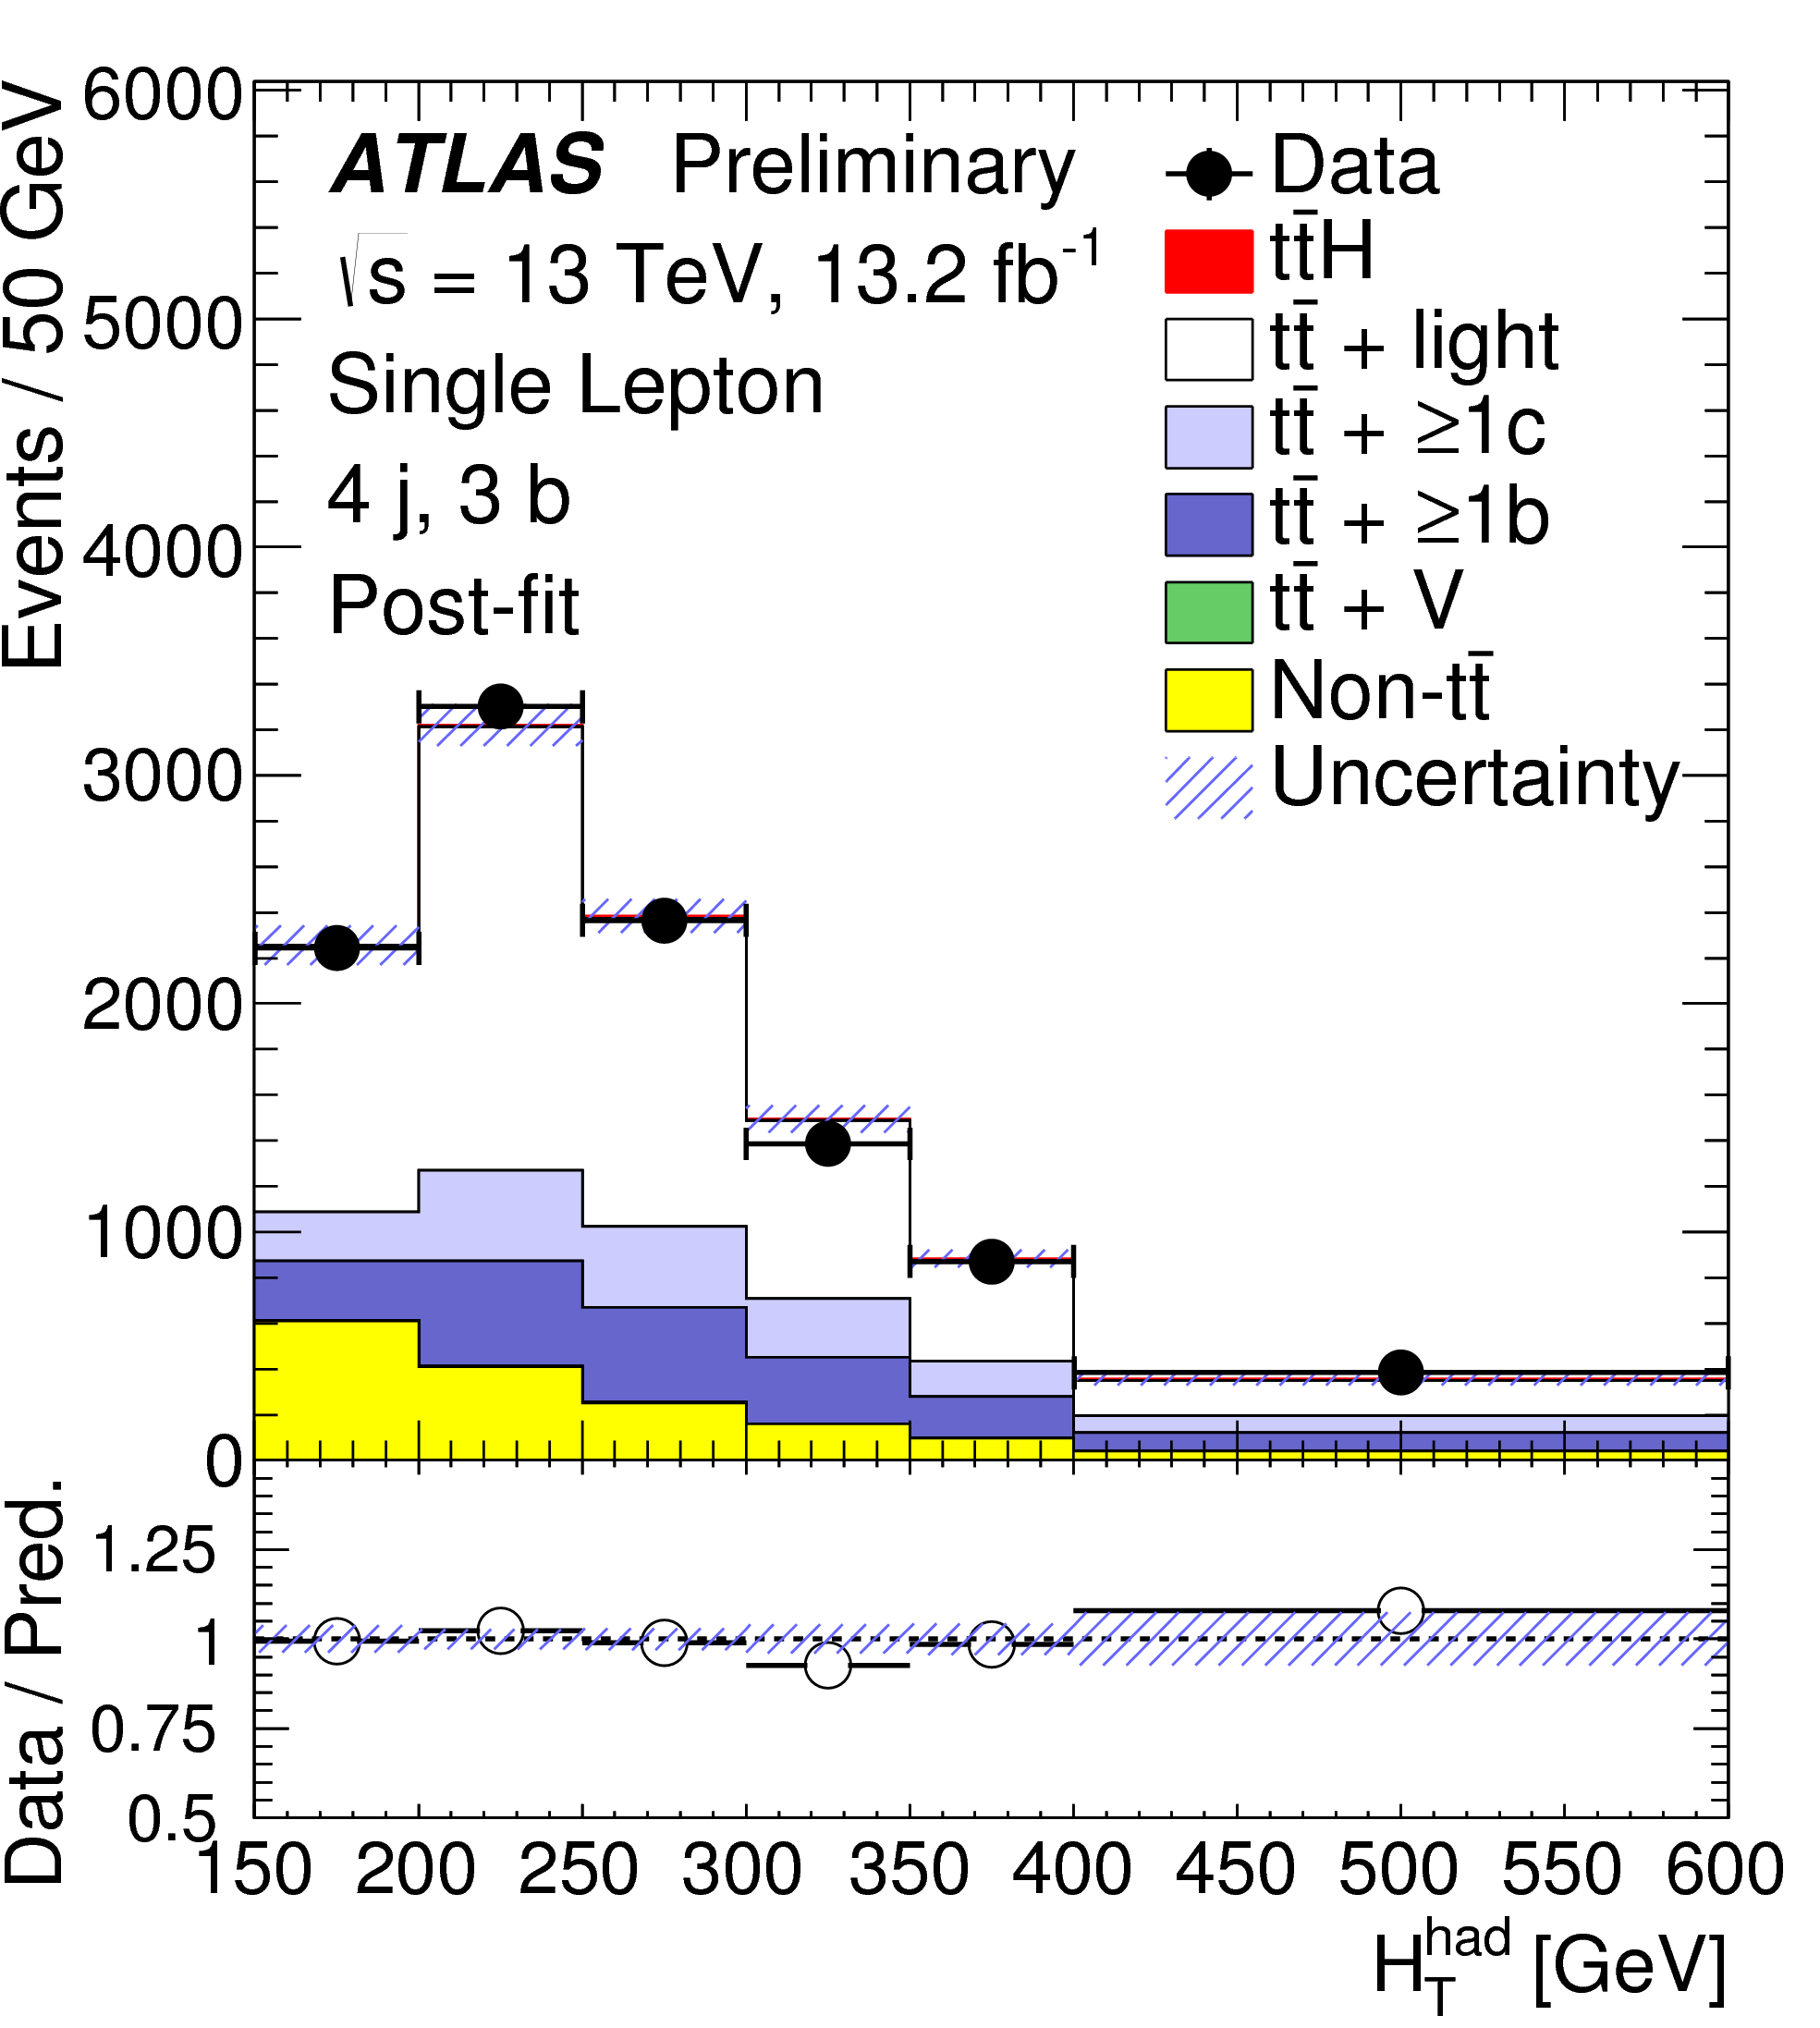
\includegraphics[width=0.9\textwidth]{figures/ttH/fig_07d.png}
  \caption{}
  \label{}
\end{subfigure}
\begin{subfigure}{0.24\textwidth}
  \centering
  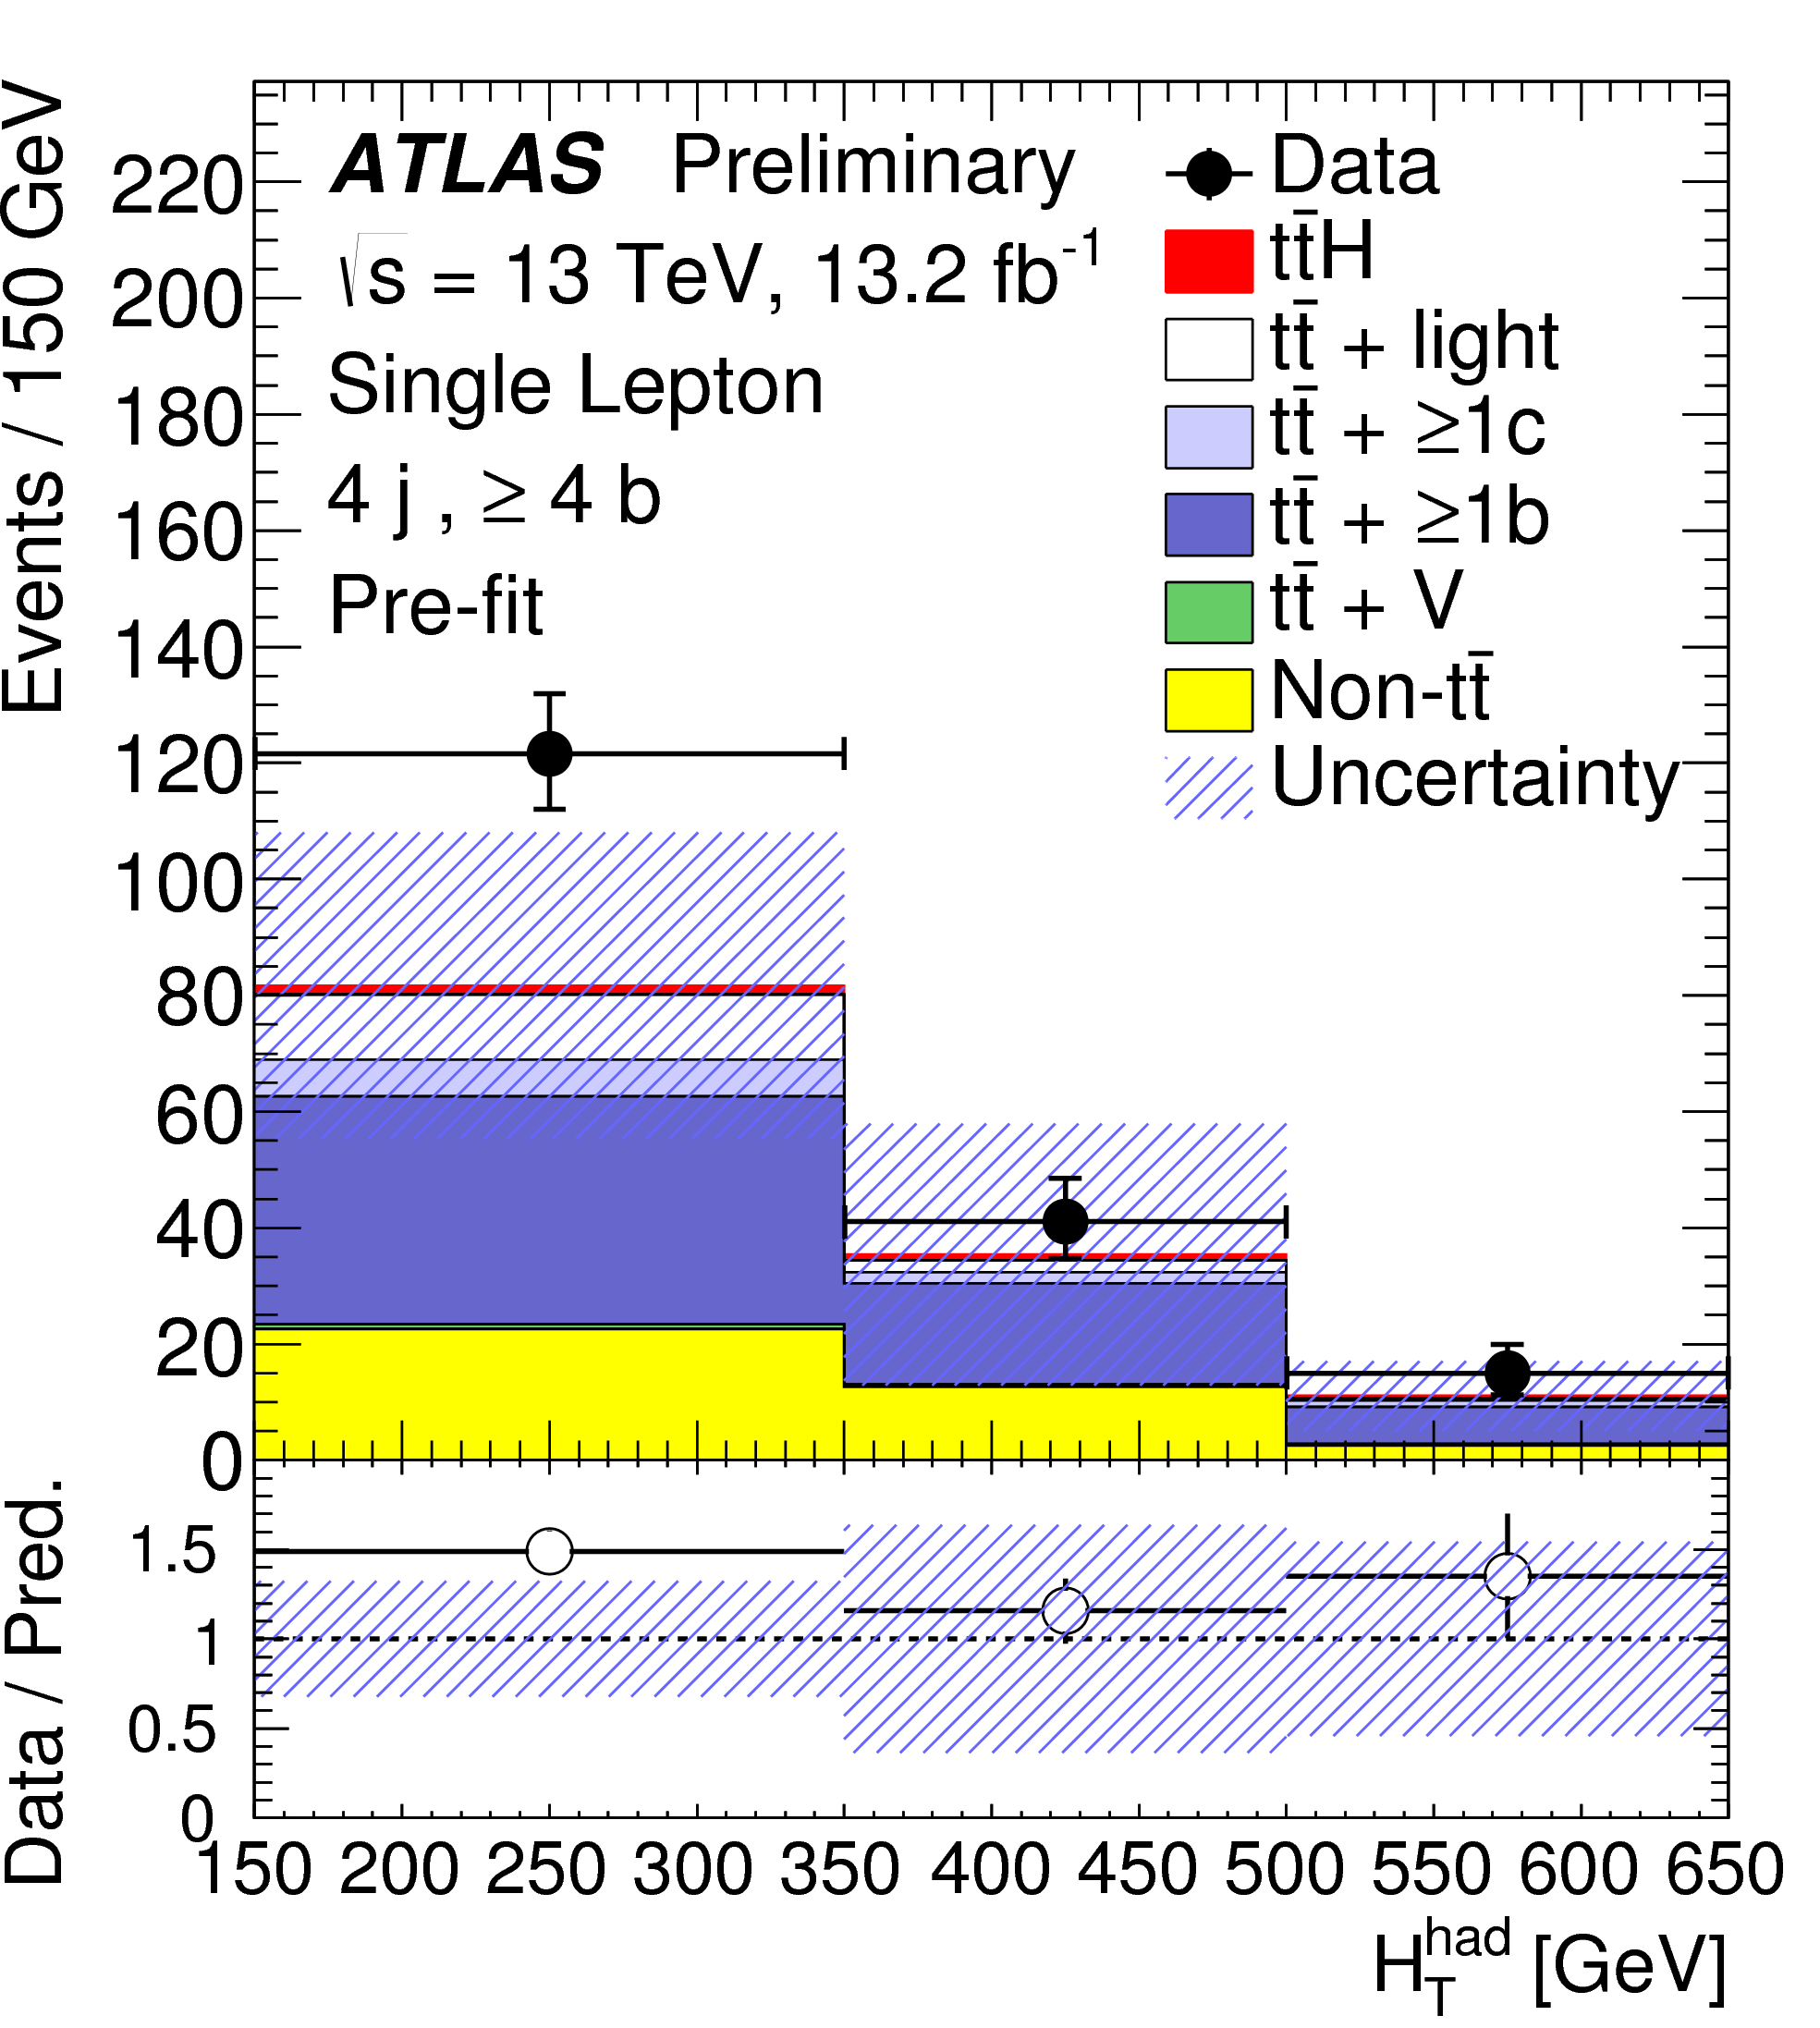
\includegraphics[width=0.9\textwidth]{figures/ttH/fig_07e.png}
  \caption{}
  \label{}
\end{subfigure}
\begin{subfigure}{0.24\textwidth}
  \centering
  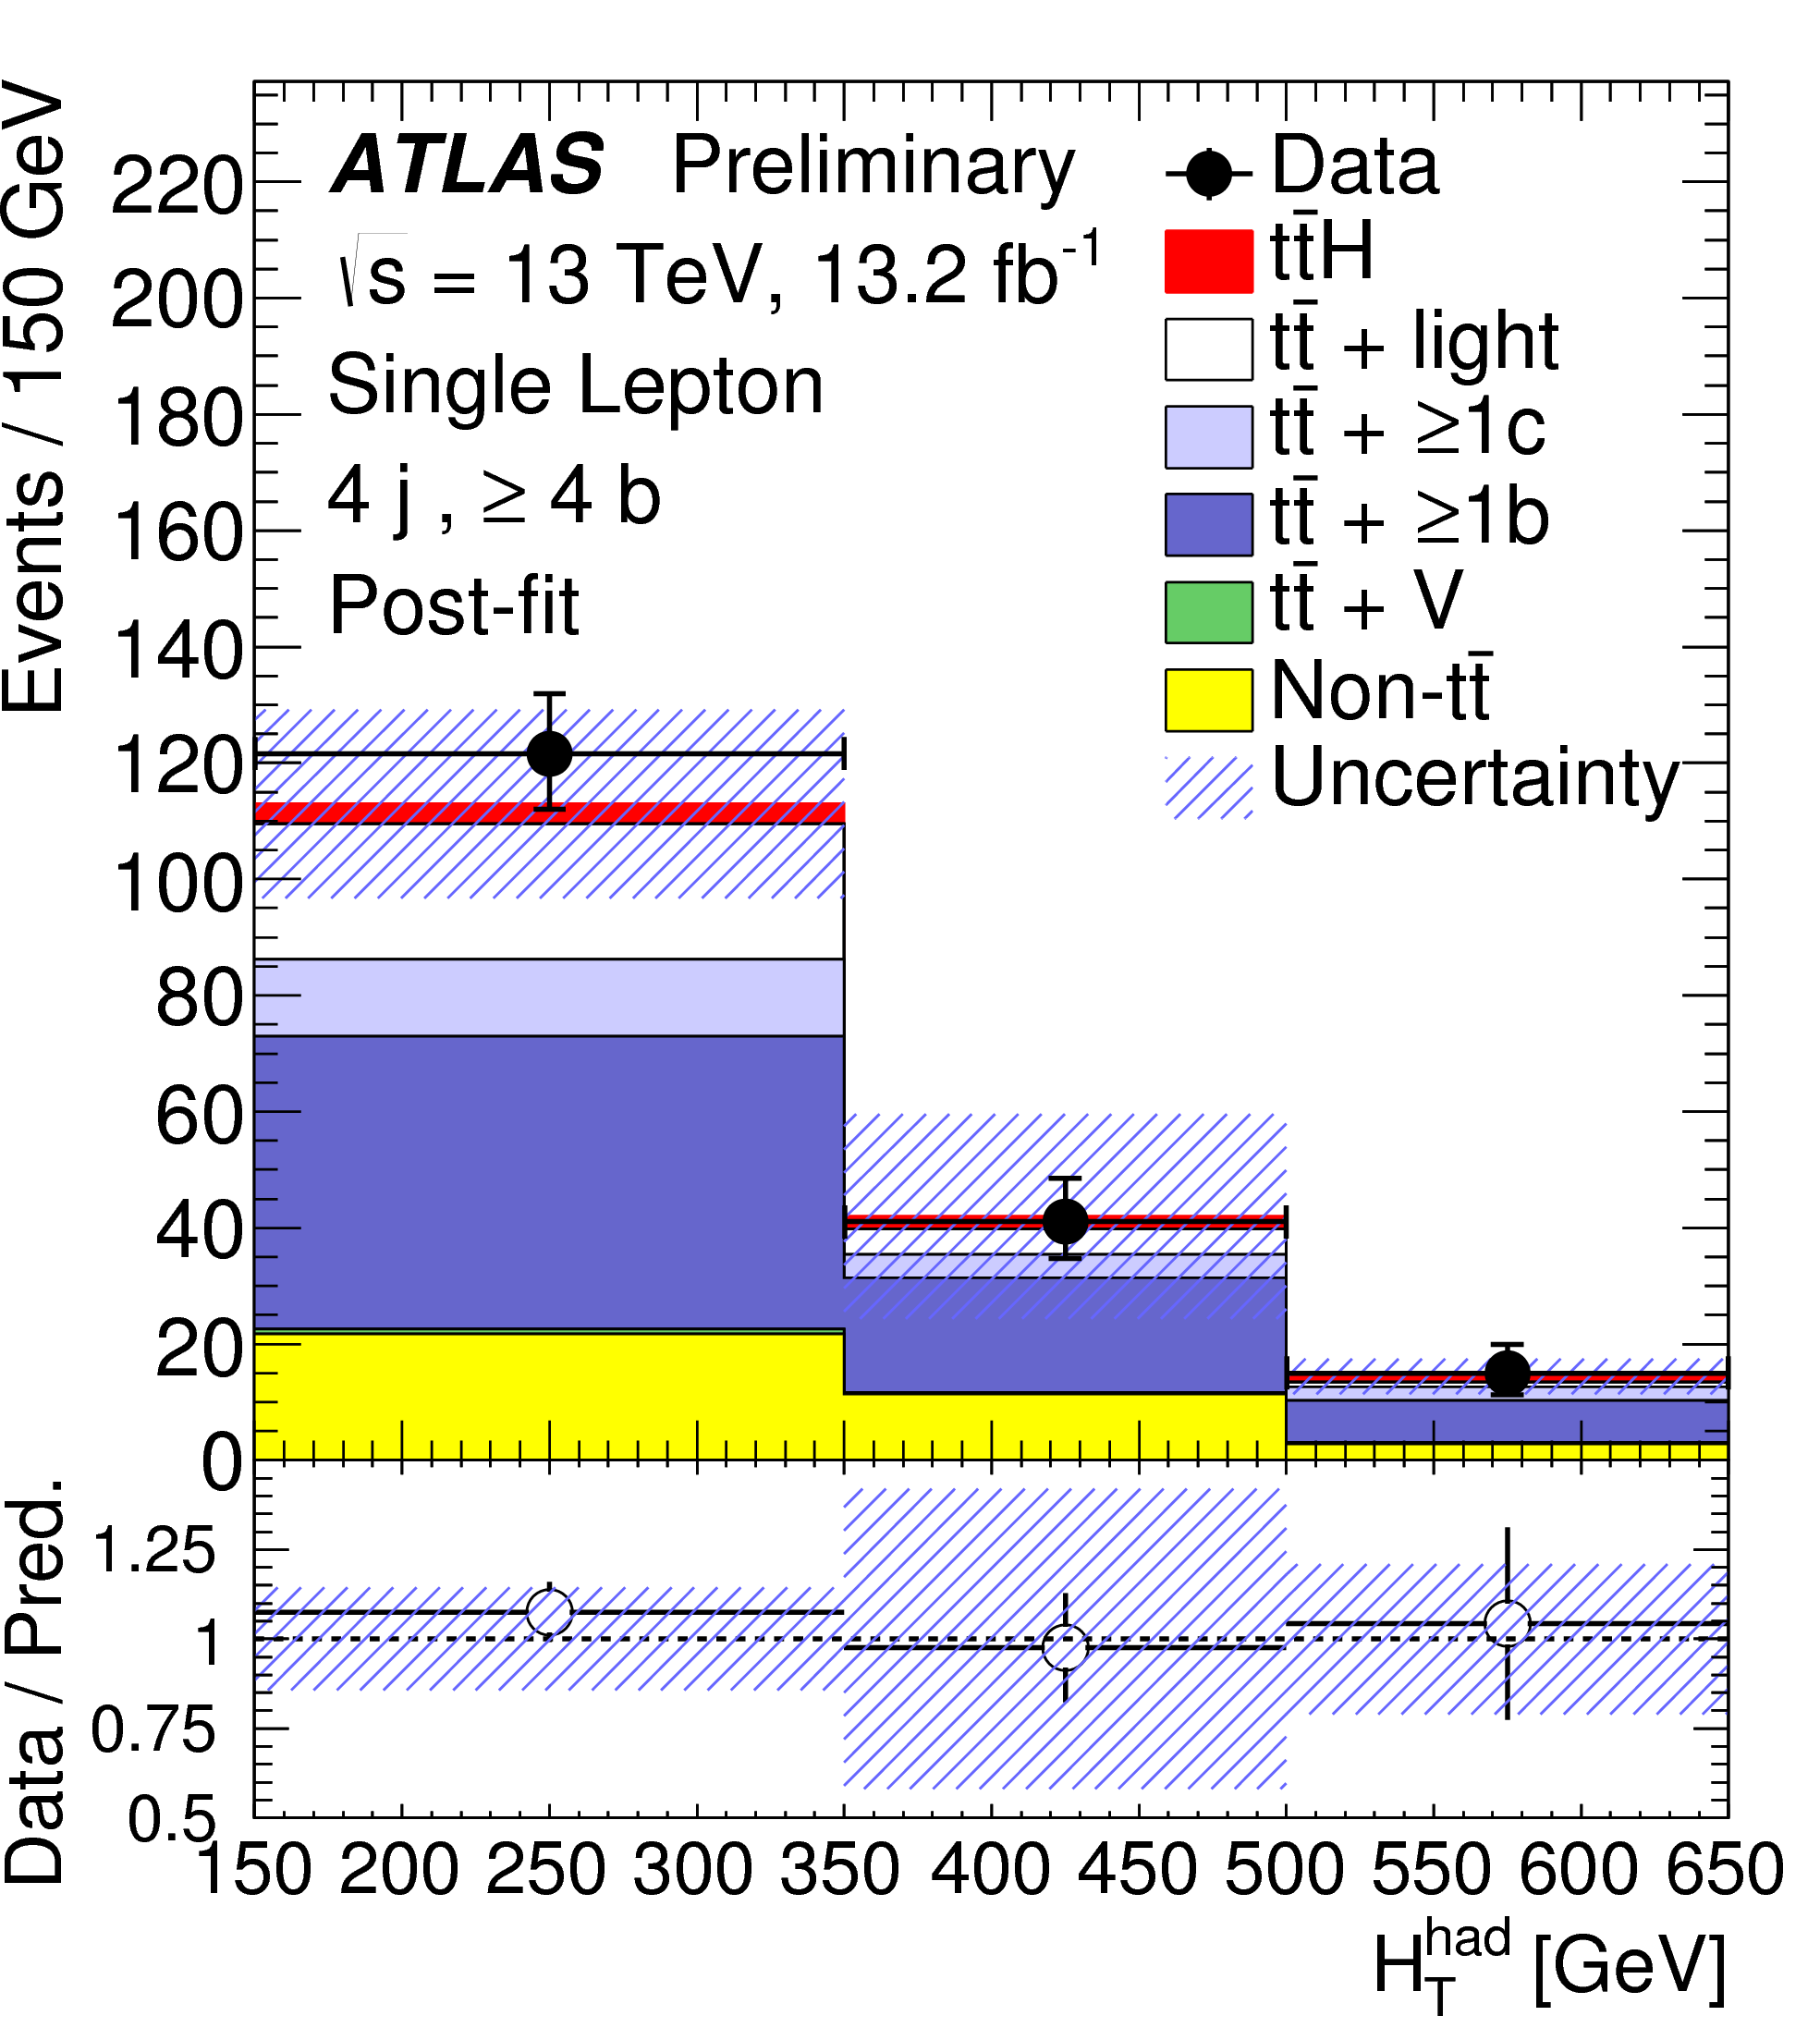
\includegraphics[width=0.9\textwidth]{figures/ttH/fig_07f.png}
  \caption{}
  \label{}
\end{subfigure}
\begin{subfigure}{0.24\textwidth}
  \centering
  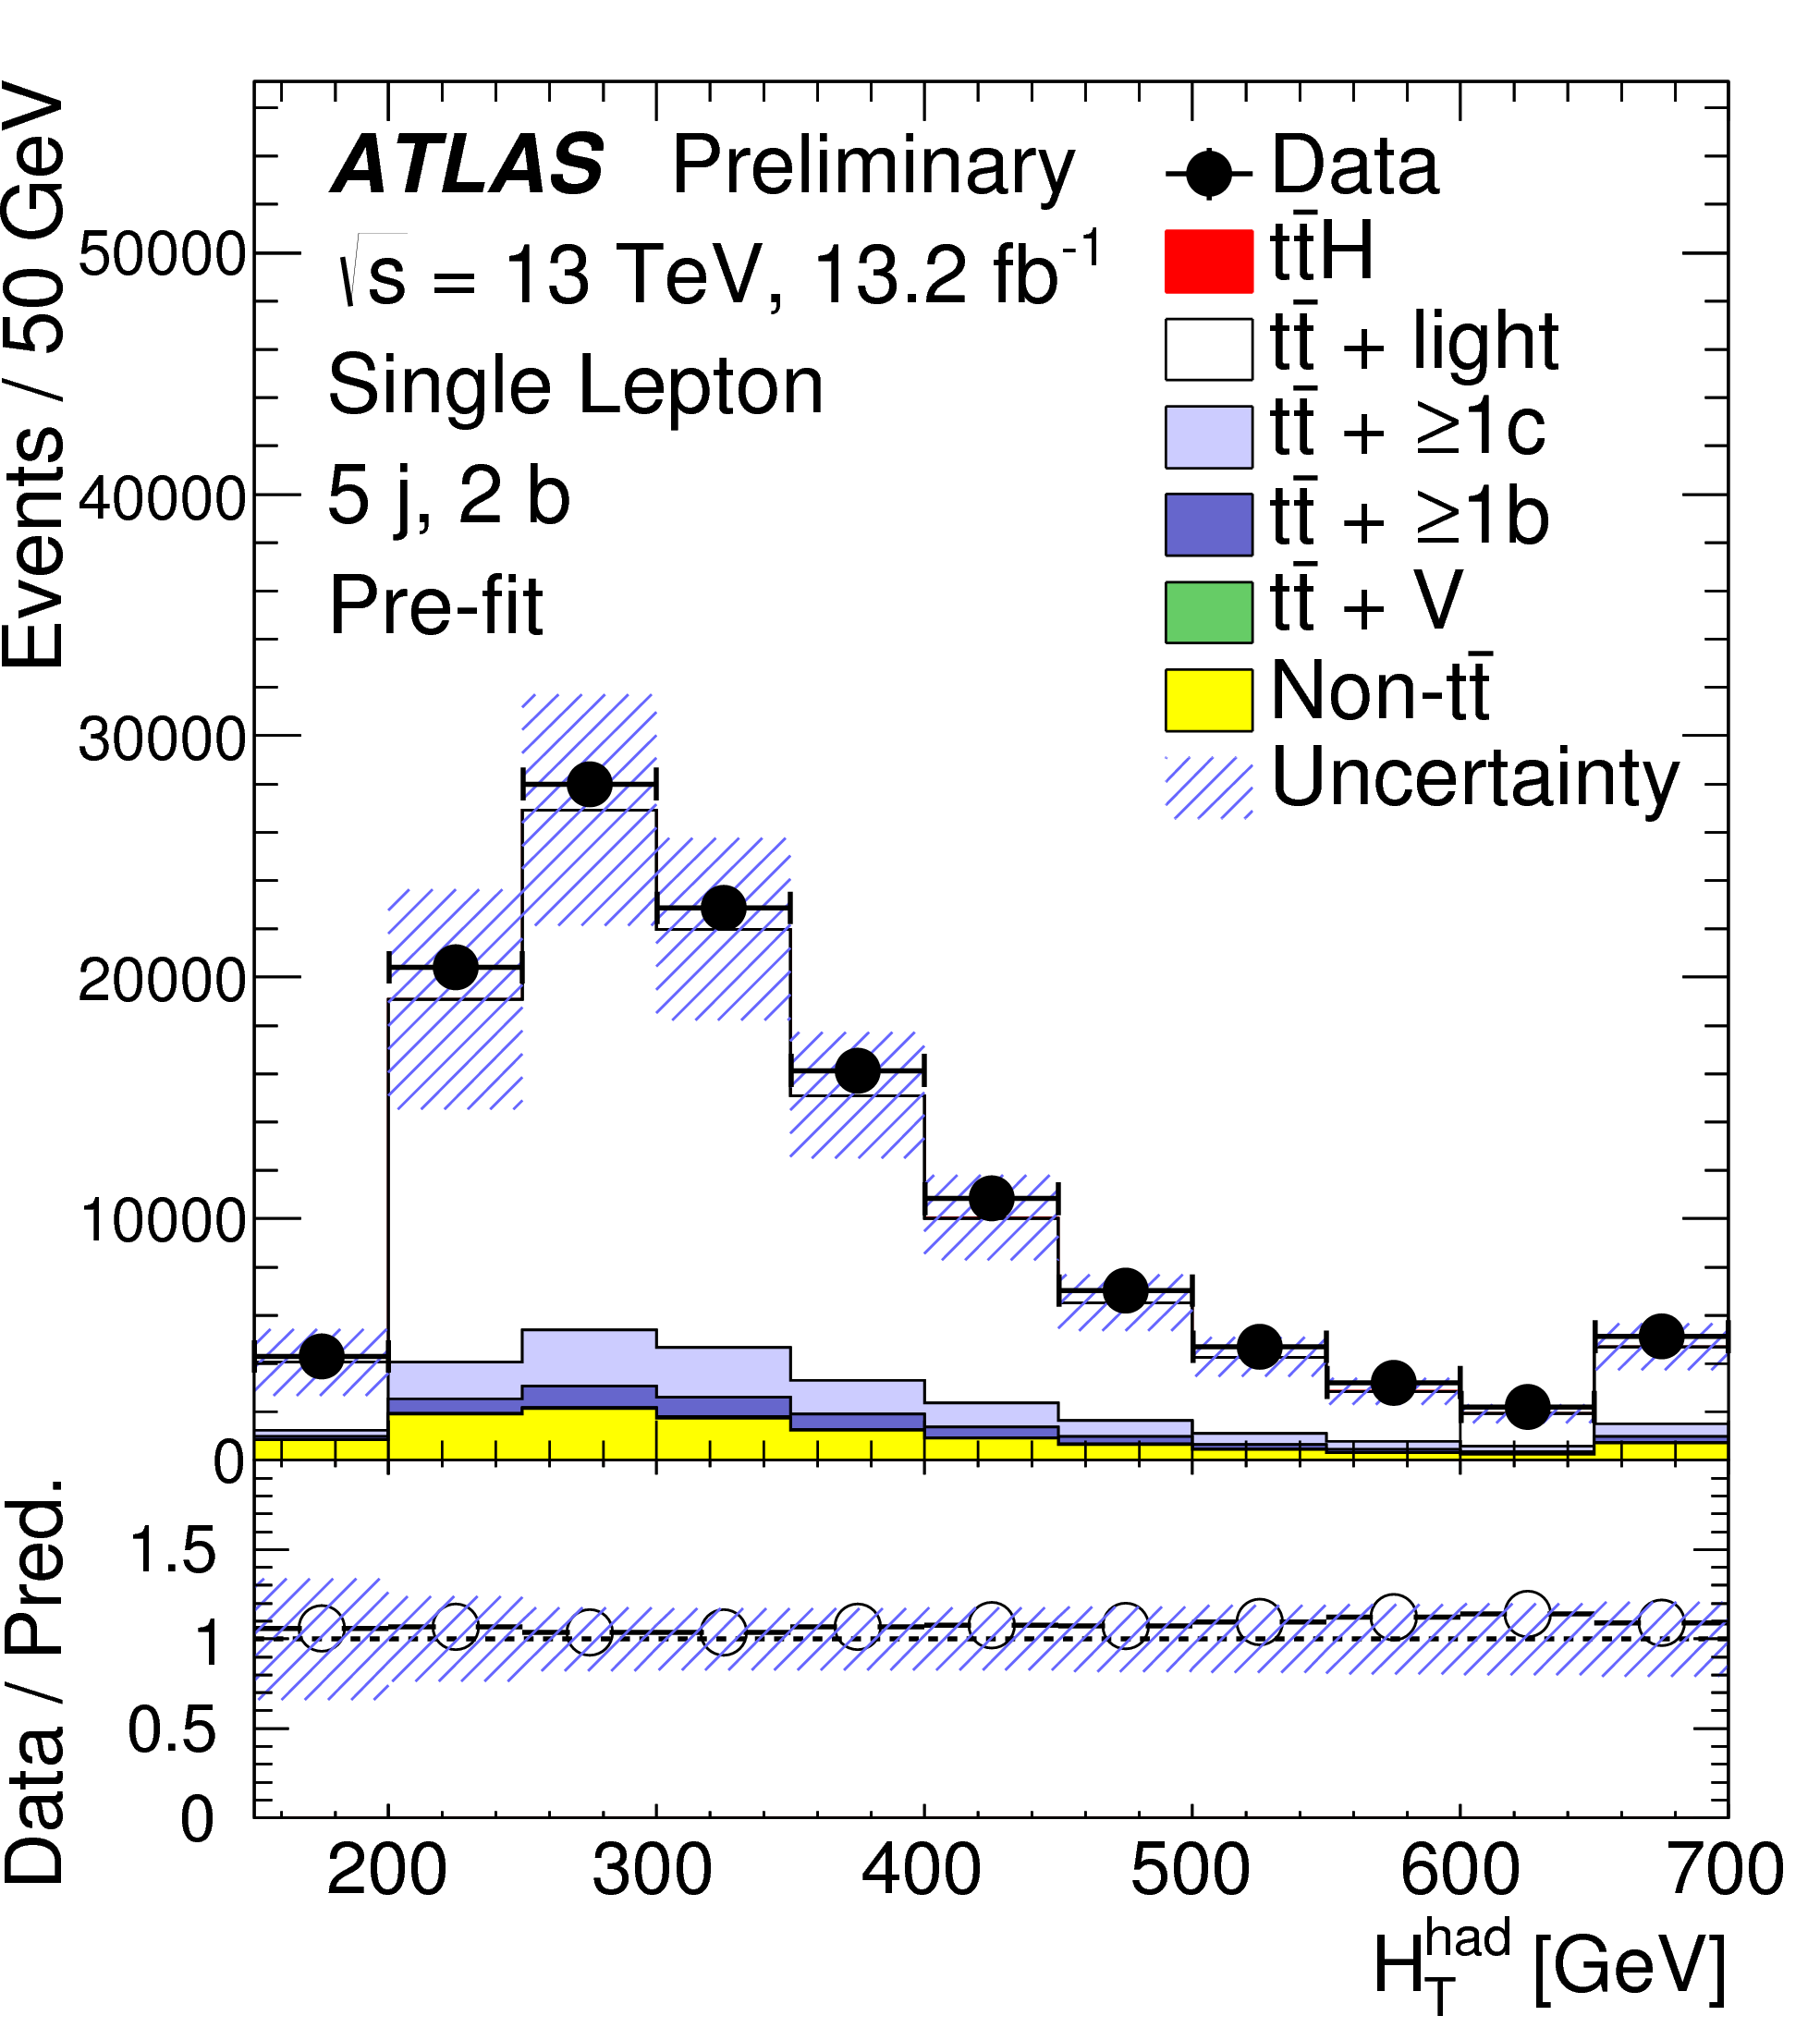
\includegraphics[width=0.9\textwidth]{figures/ttH/fig_08a.png}
  \caption{}
  \label{}
\end{subfigure}
\begin{subfigure}{0.24\textwidth}
  \centering
  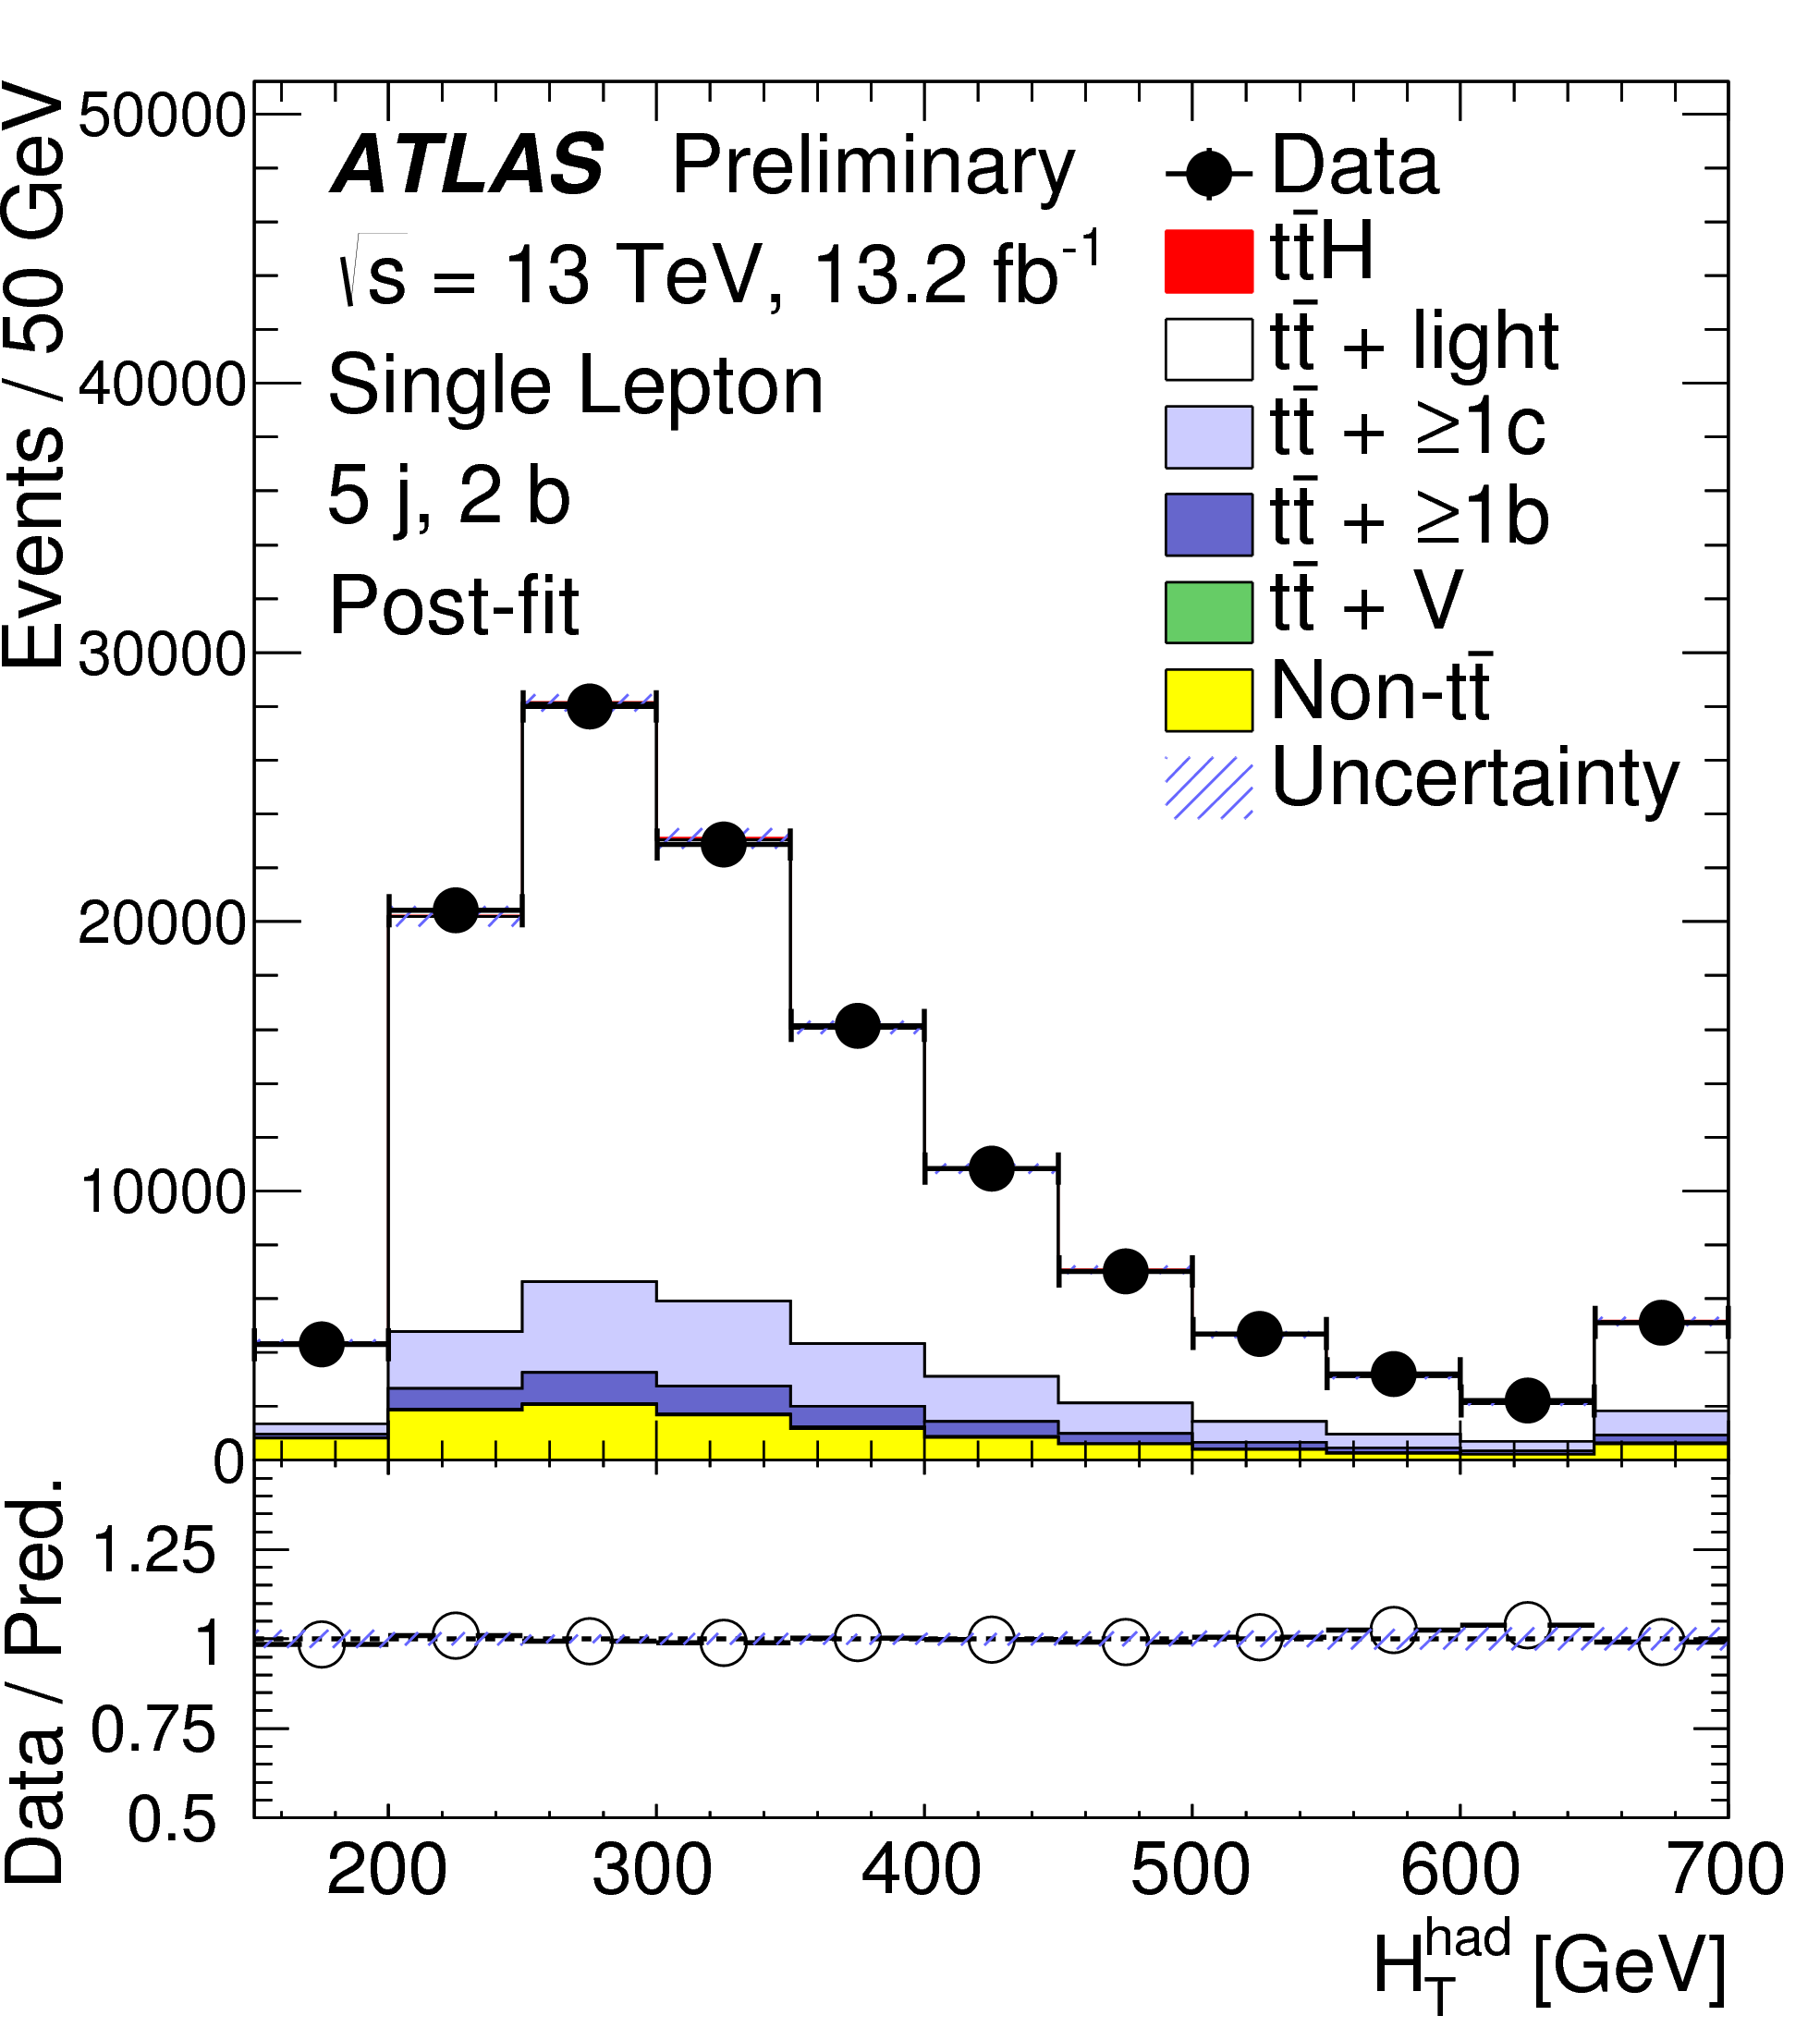
\includegraphics[width=0.9\textwidth]{figures/ttH/fig_08b.png}
  \caption{}
  \label{}
\end{subfigure}
\begin{subfigure}{0.24\textwidth}
  \centering
  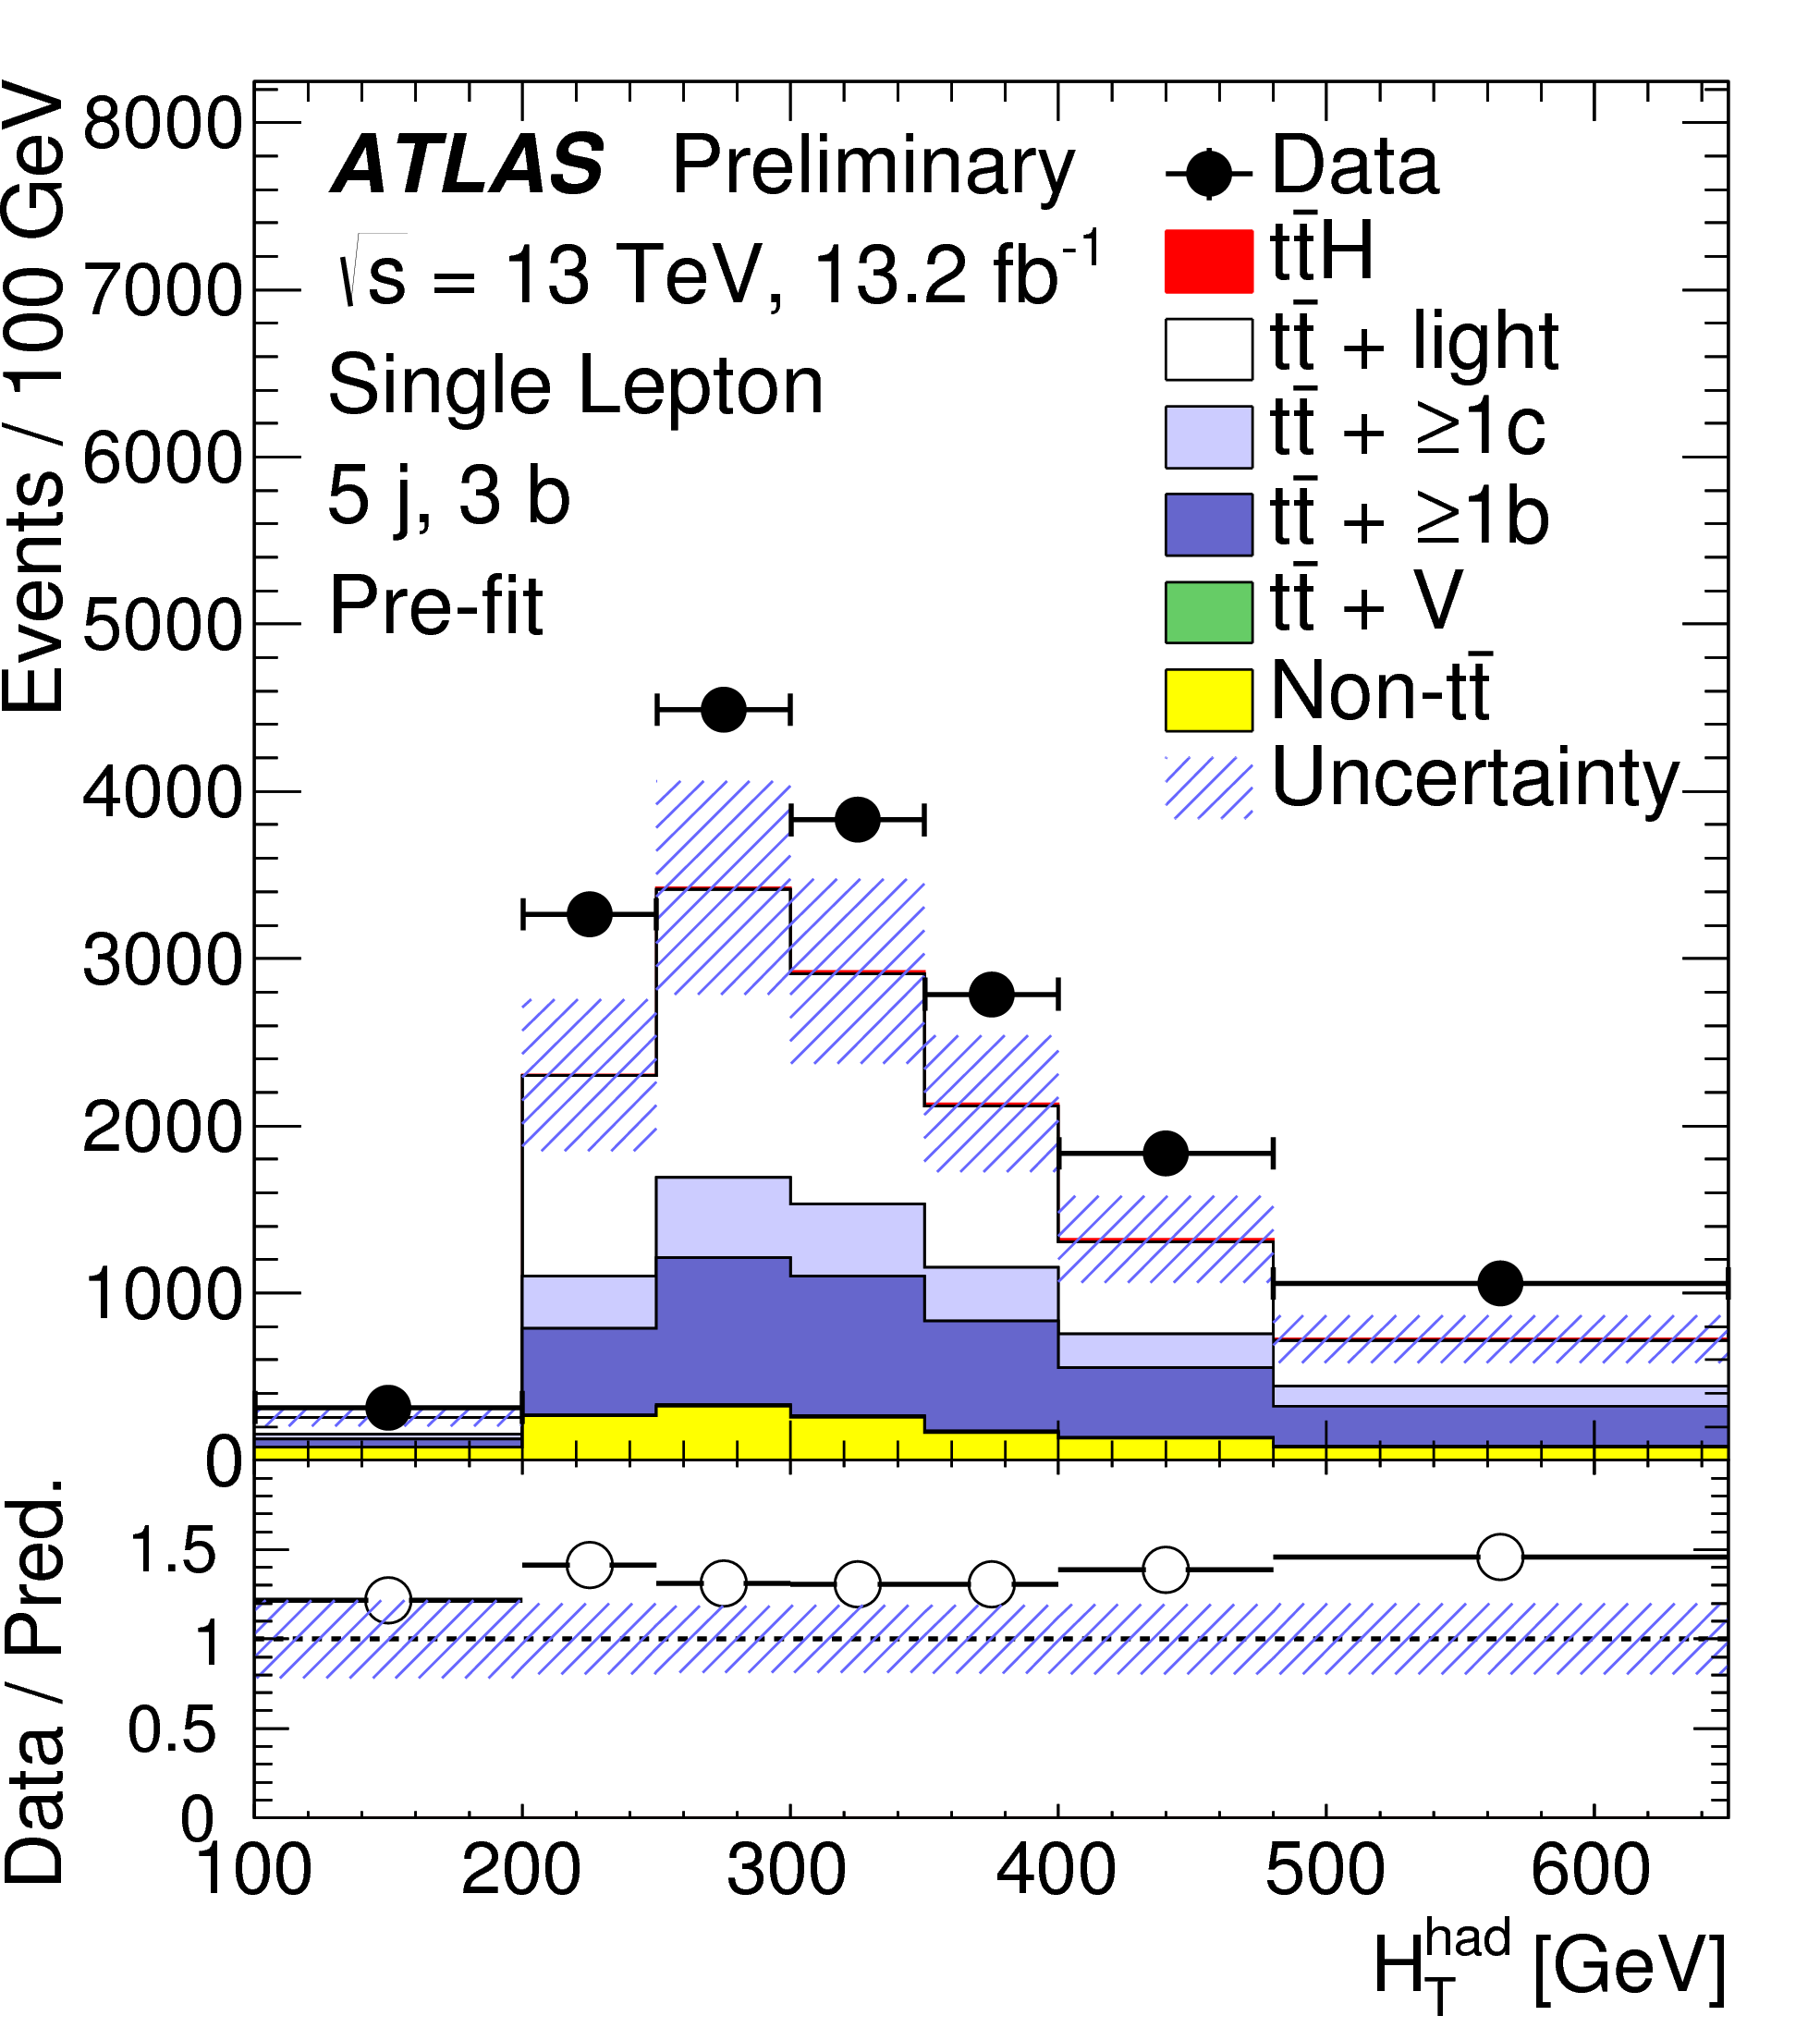
\includegraphics[width=0.9\textwidth]{figures/ttH/fig_08c.png}
  \caption{}
  \label{}
\end{subfigure}
\begin{subfigure}{0.24\textwidth}
  \centering
  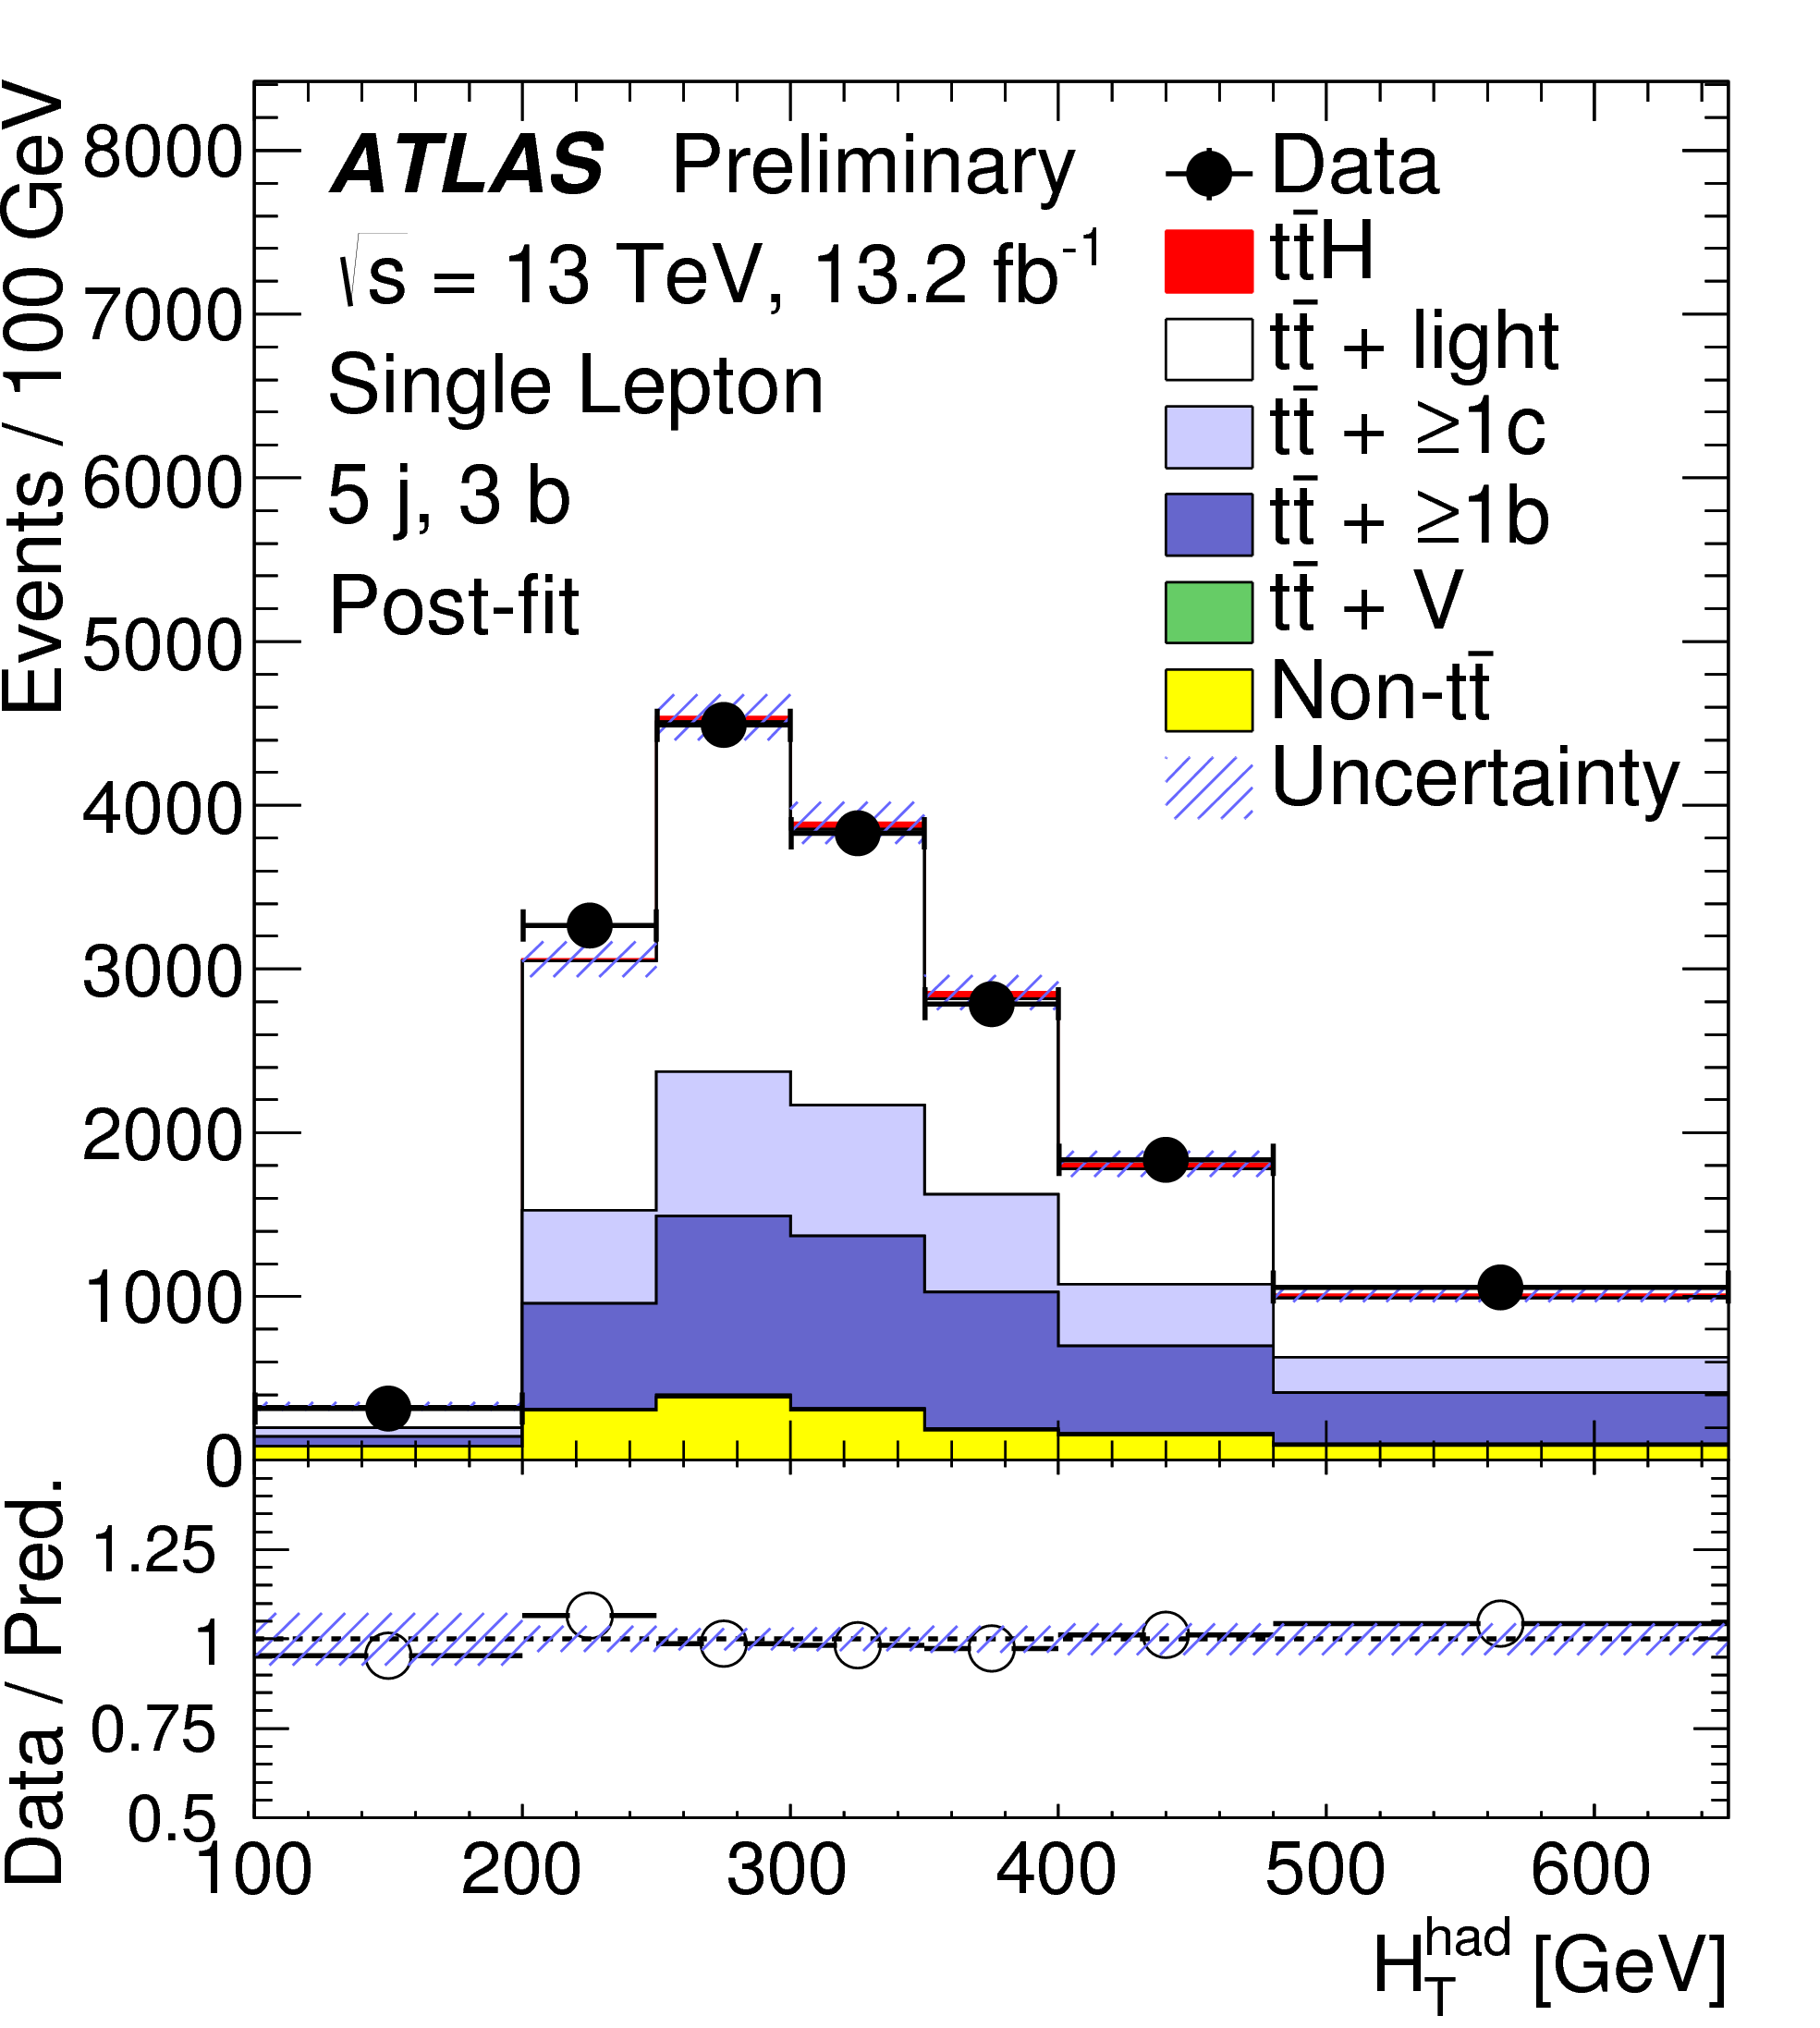
\includegraphics[width=0.9\textwidth]{figures/ttH/fig_08d.png}
  \caption{}
  \label{}
\end{subfigure}
\begin{subfigure}{0.24\textwidth}
  \centering
  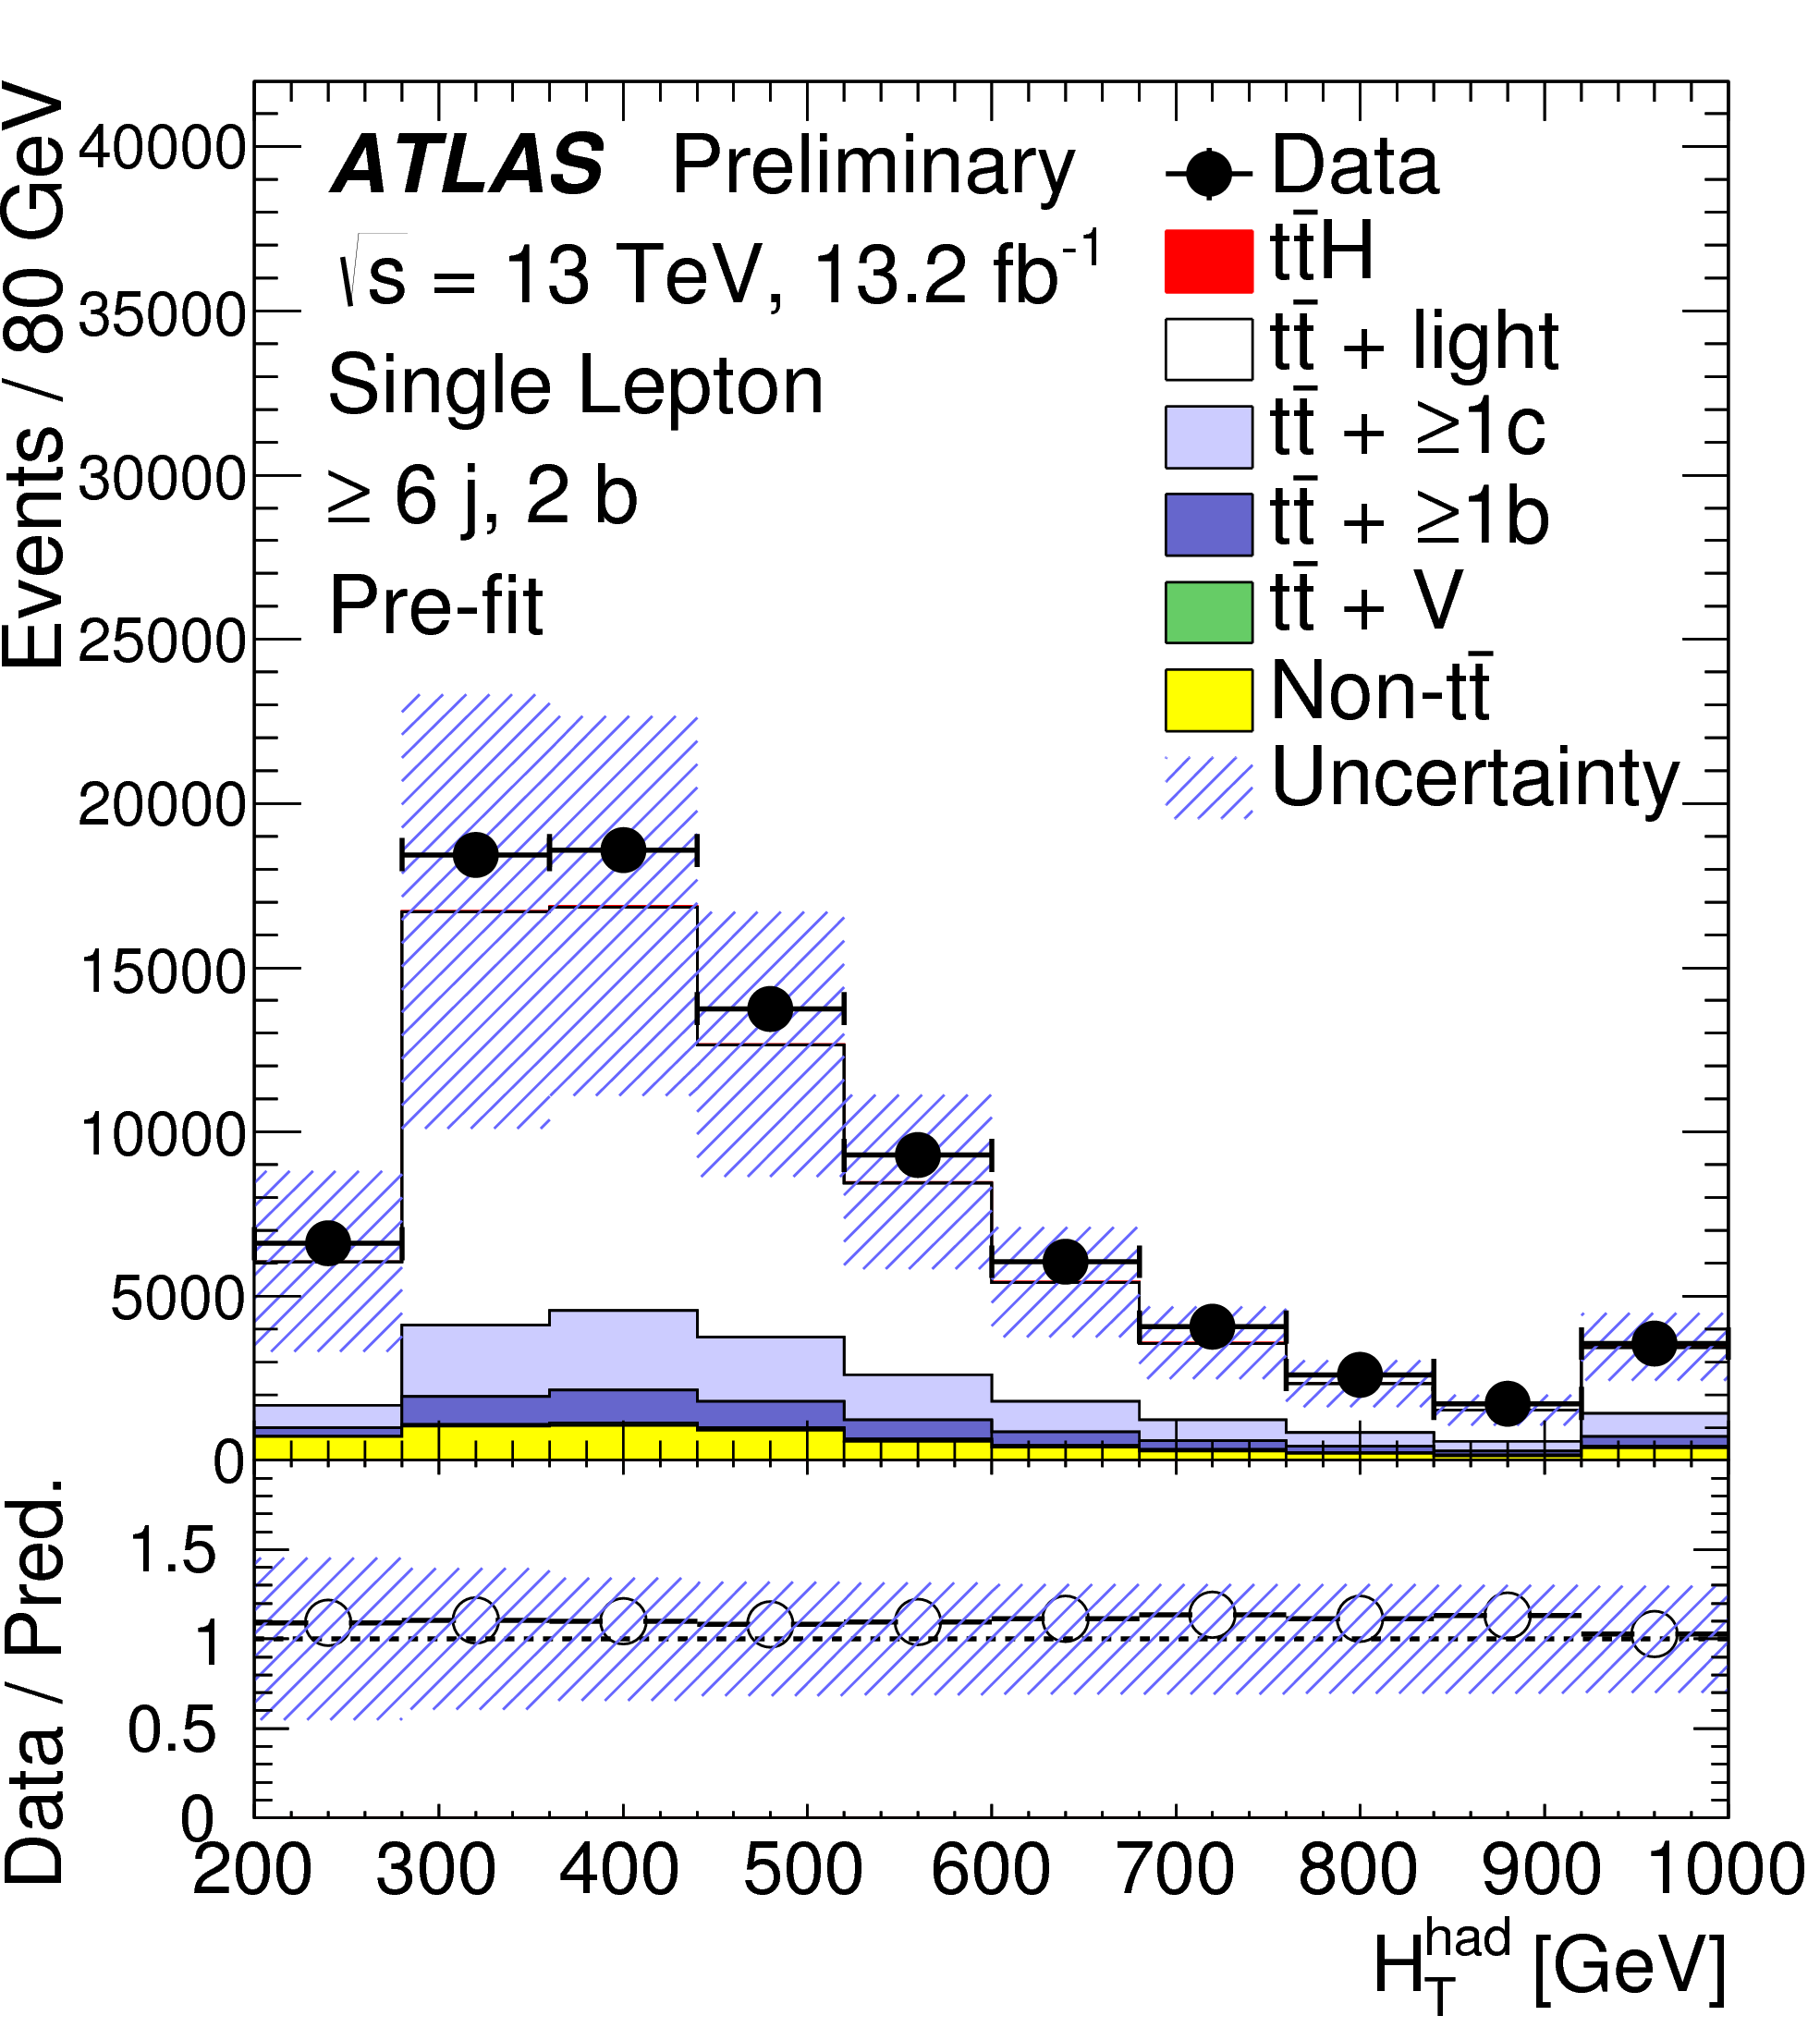
\includegraphics[width=0.9\textwidth]{figures/ttH/fig_08e.png}
  \caption{}
  \label{}
\end{subfigure}
\begin{subfigure}{0.24\textwidth}
  \centering
  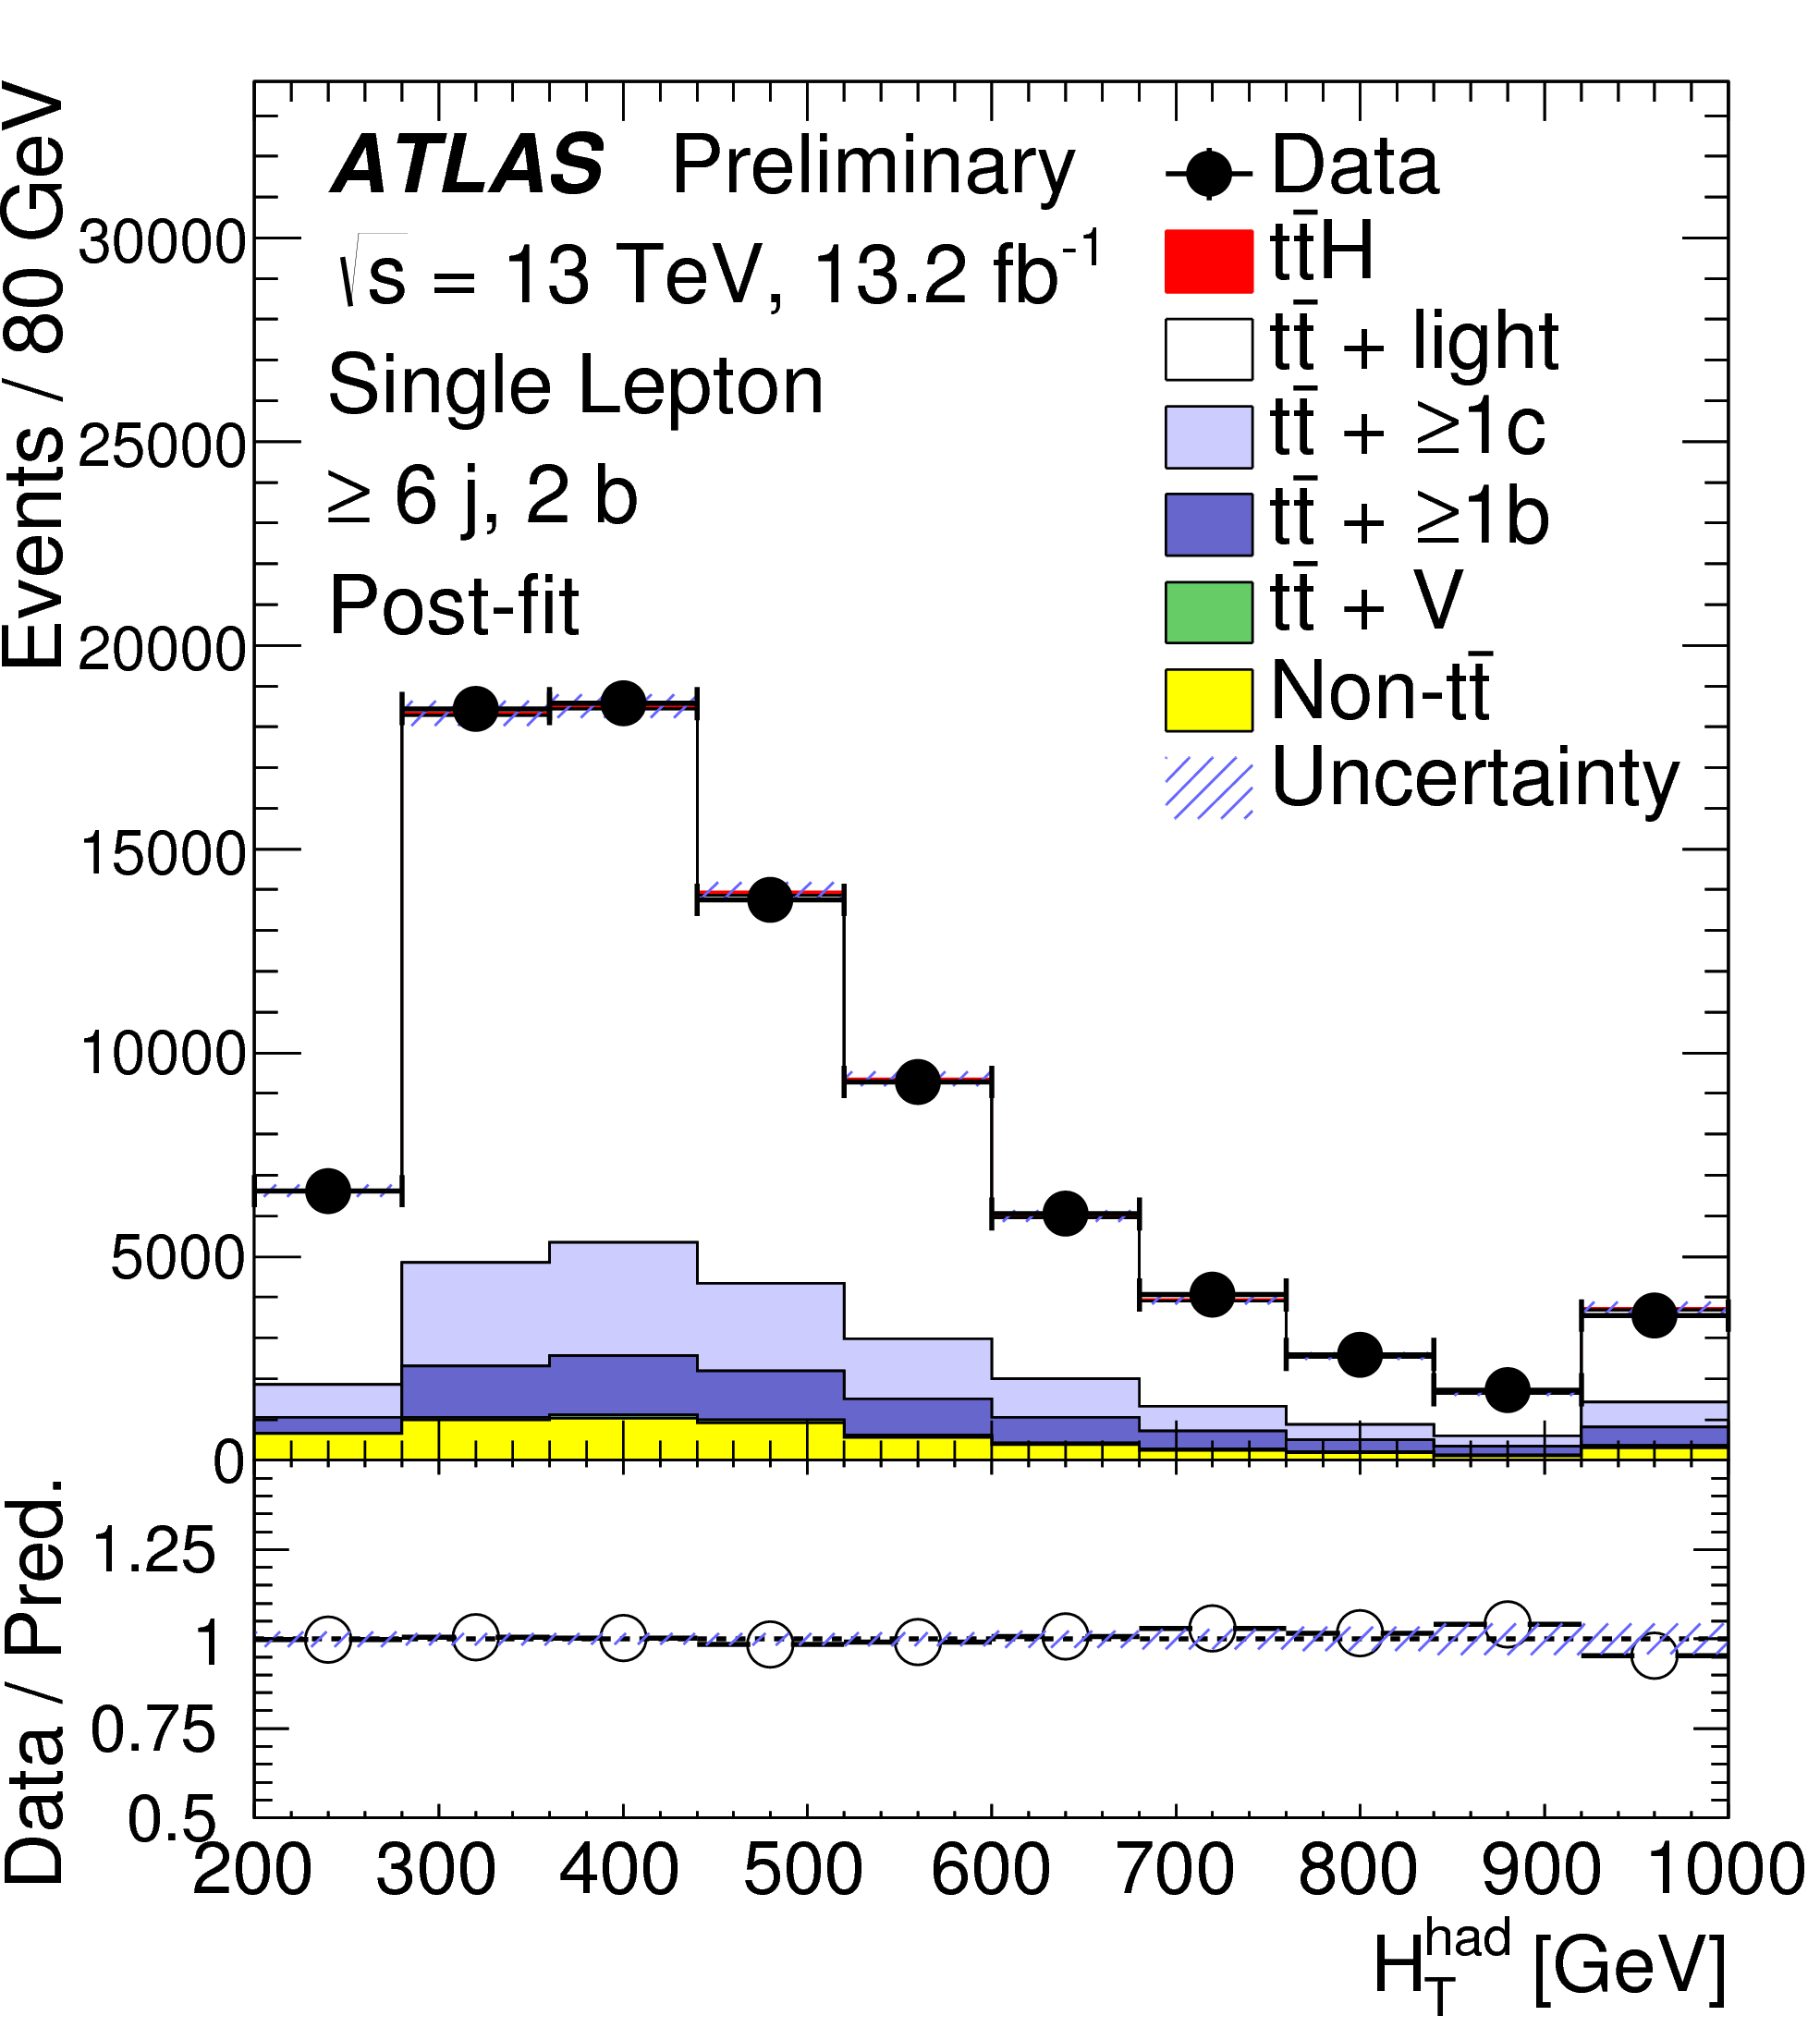
\includegraphics[width=0.9\textwidth]{figures/ttH/fig_08f.png}
  \caption{}
  \label{}
\end{subfigure}

\captionsetup{width=0.85\textwidth}  \caption{\small Comparison between the data and prediction for the $H_{\rm T}^{\rm had}$ distributions before and after performing the combined fit to data in the single-lepton and dilepton channels (``Pre-fit'' and ``Post-fit'', respectively) under the signal-plus-background hypothesis. Shown are the (4j, 2b) region (a) pre-fit and (b) post-fit, the (4j, 3b) region (c) pre-fit and (d) post-fit, the (4j, $\ge$4b) region (e) pre-fit and (f) post-fit, the (5j, 2b)  region (g) pre-fit and (h) post-fit, the (5j, 3b)  region (i) pre-fit and (j) post-fit, and the ($\ge$6j, 2b) region (k) pre-fit and (l) post-fit.
The small contributions from single top, $W/Z$+jets, diboson, and multijet backgrounds are combined into a single background source  referred to as ``Non-$t\bar{t}$''. The last bin in all figures contains the overflow. The bottom panels display the ratios of data to the total background prediction (``Bkg''). The blue triangles indicate points that are outside the vertical range of the figure. The hashed area represents the total uncertainty on the background. In the case of the pre-fit background uncertainty, the normalisation uncertainties on the $t\bar{t}+\ge1b$ and $t\bar{t}+\ge1c$ backgrounds are not included.}
\label{sec:tth:fig:hthad1}
\end{figure}

\begin{figure}[htbp!]
\begin{subfigure}{0.24\textwidth}
  \centering
  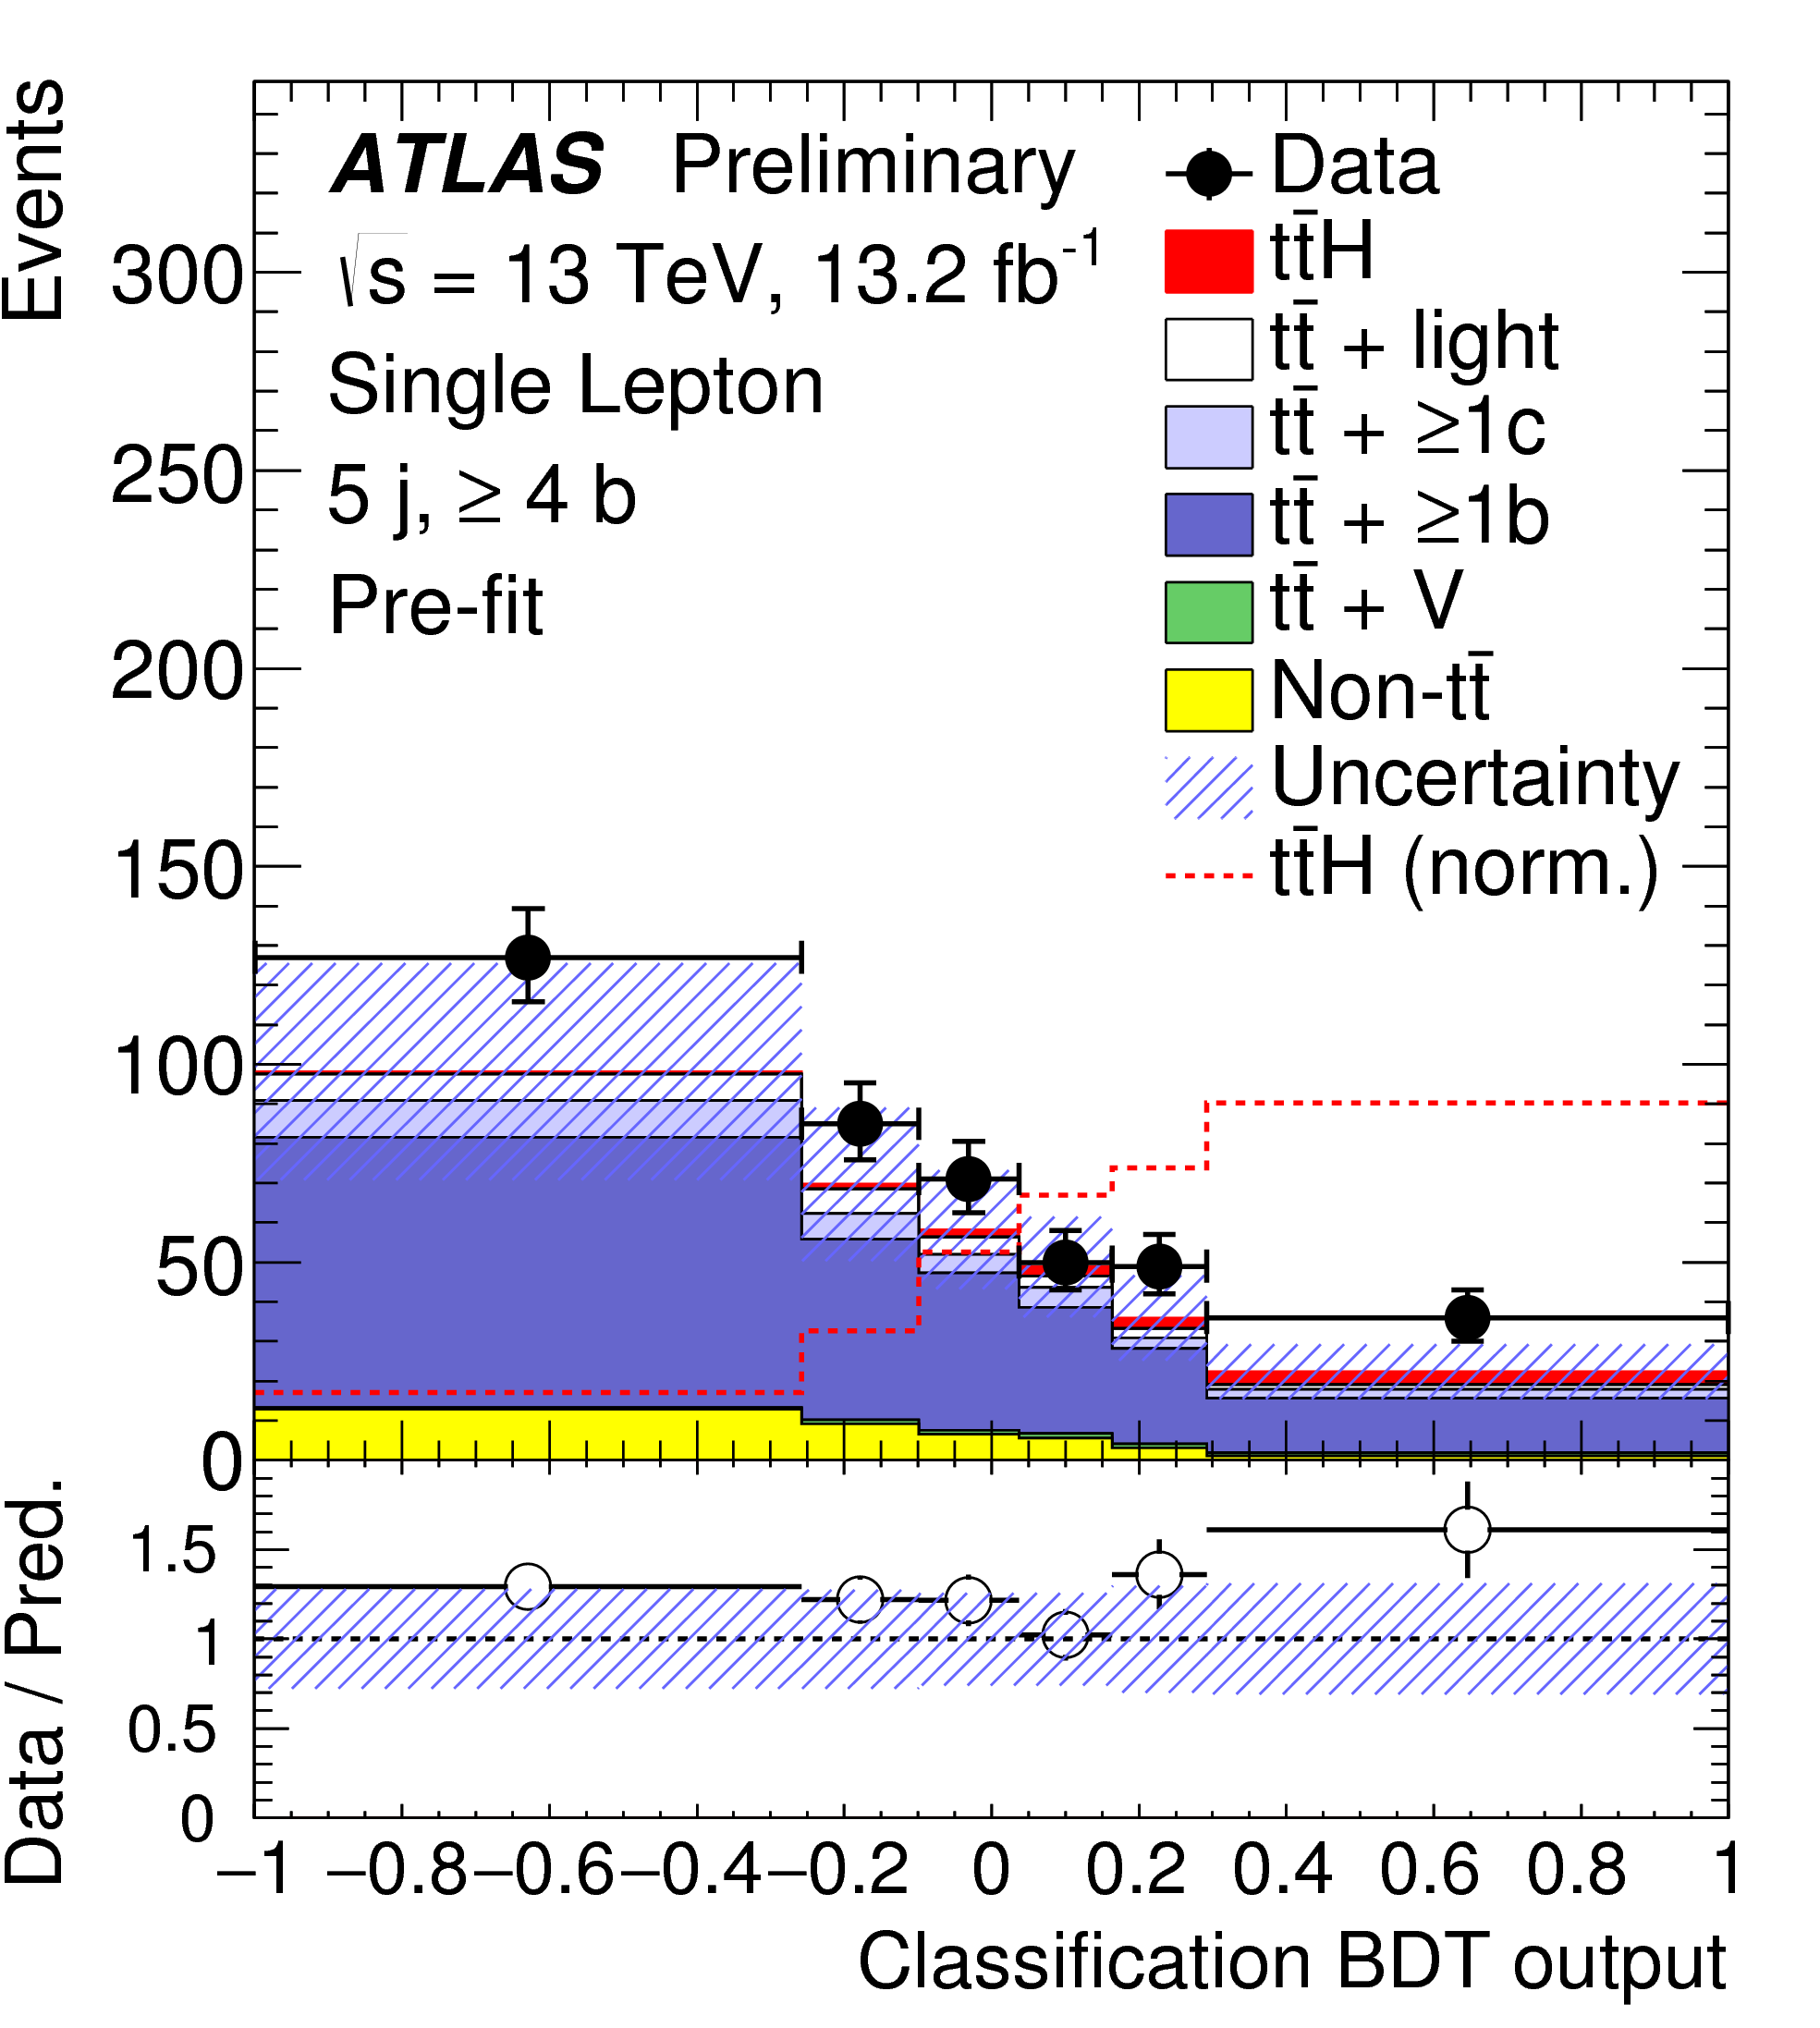
\includegraphics[width=0.9\textwidth]{figures/ttH/fig_11a.png}
  \caption{}
  \label{}
\end{subfigure}
\begin{subfigure}{0.24\textwidth}
  \centering
  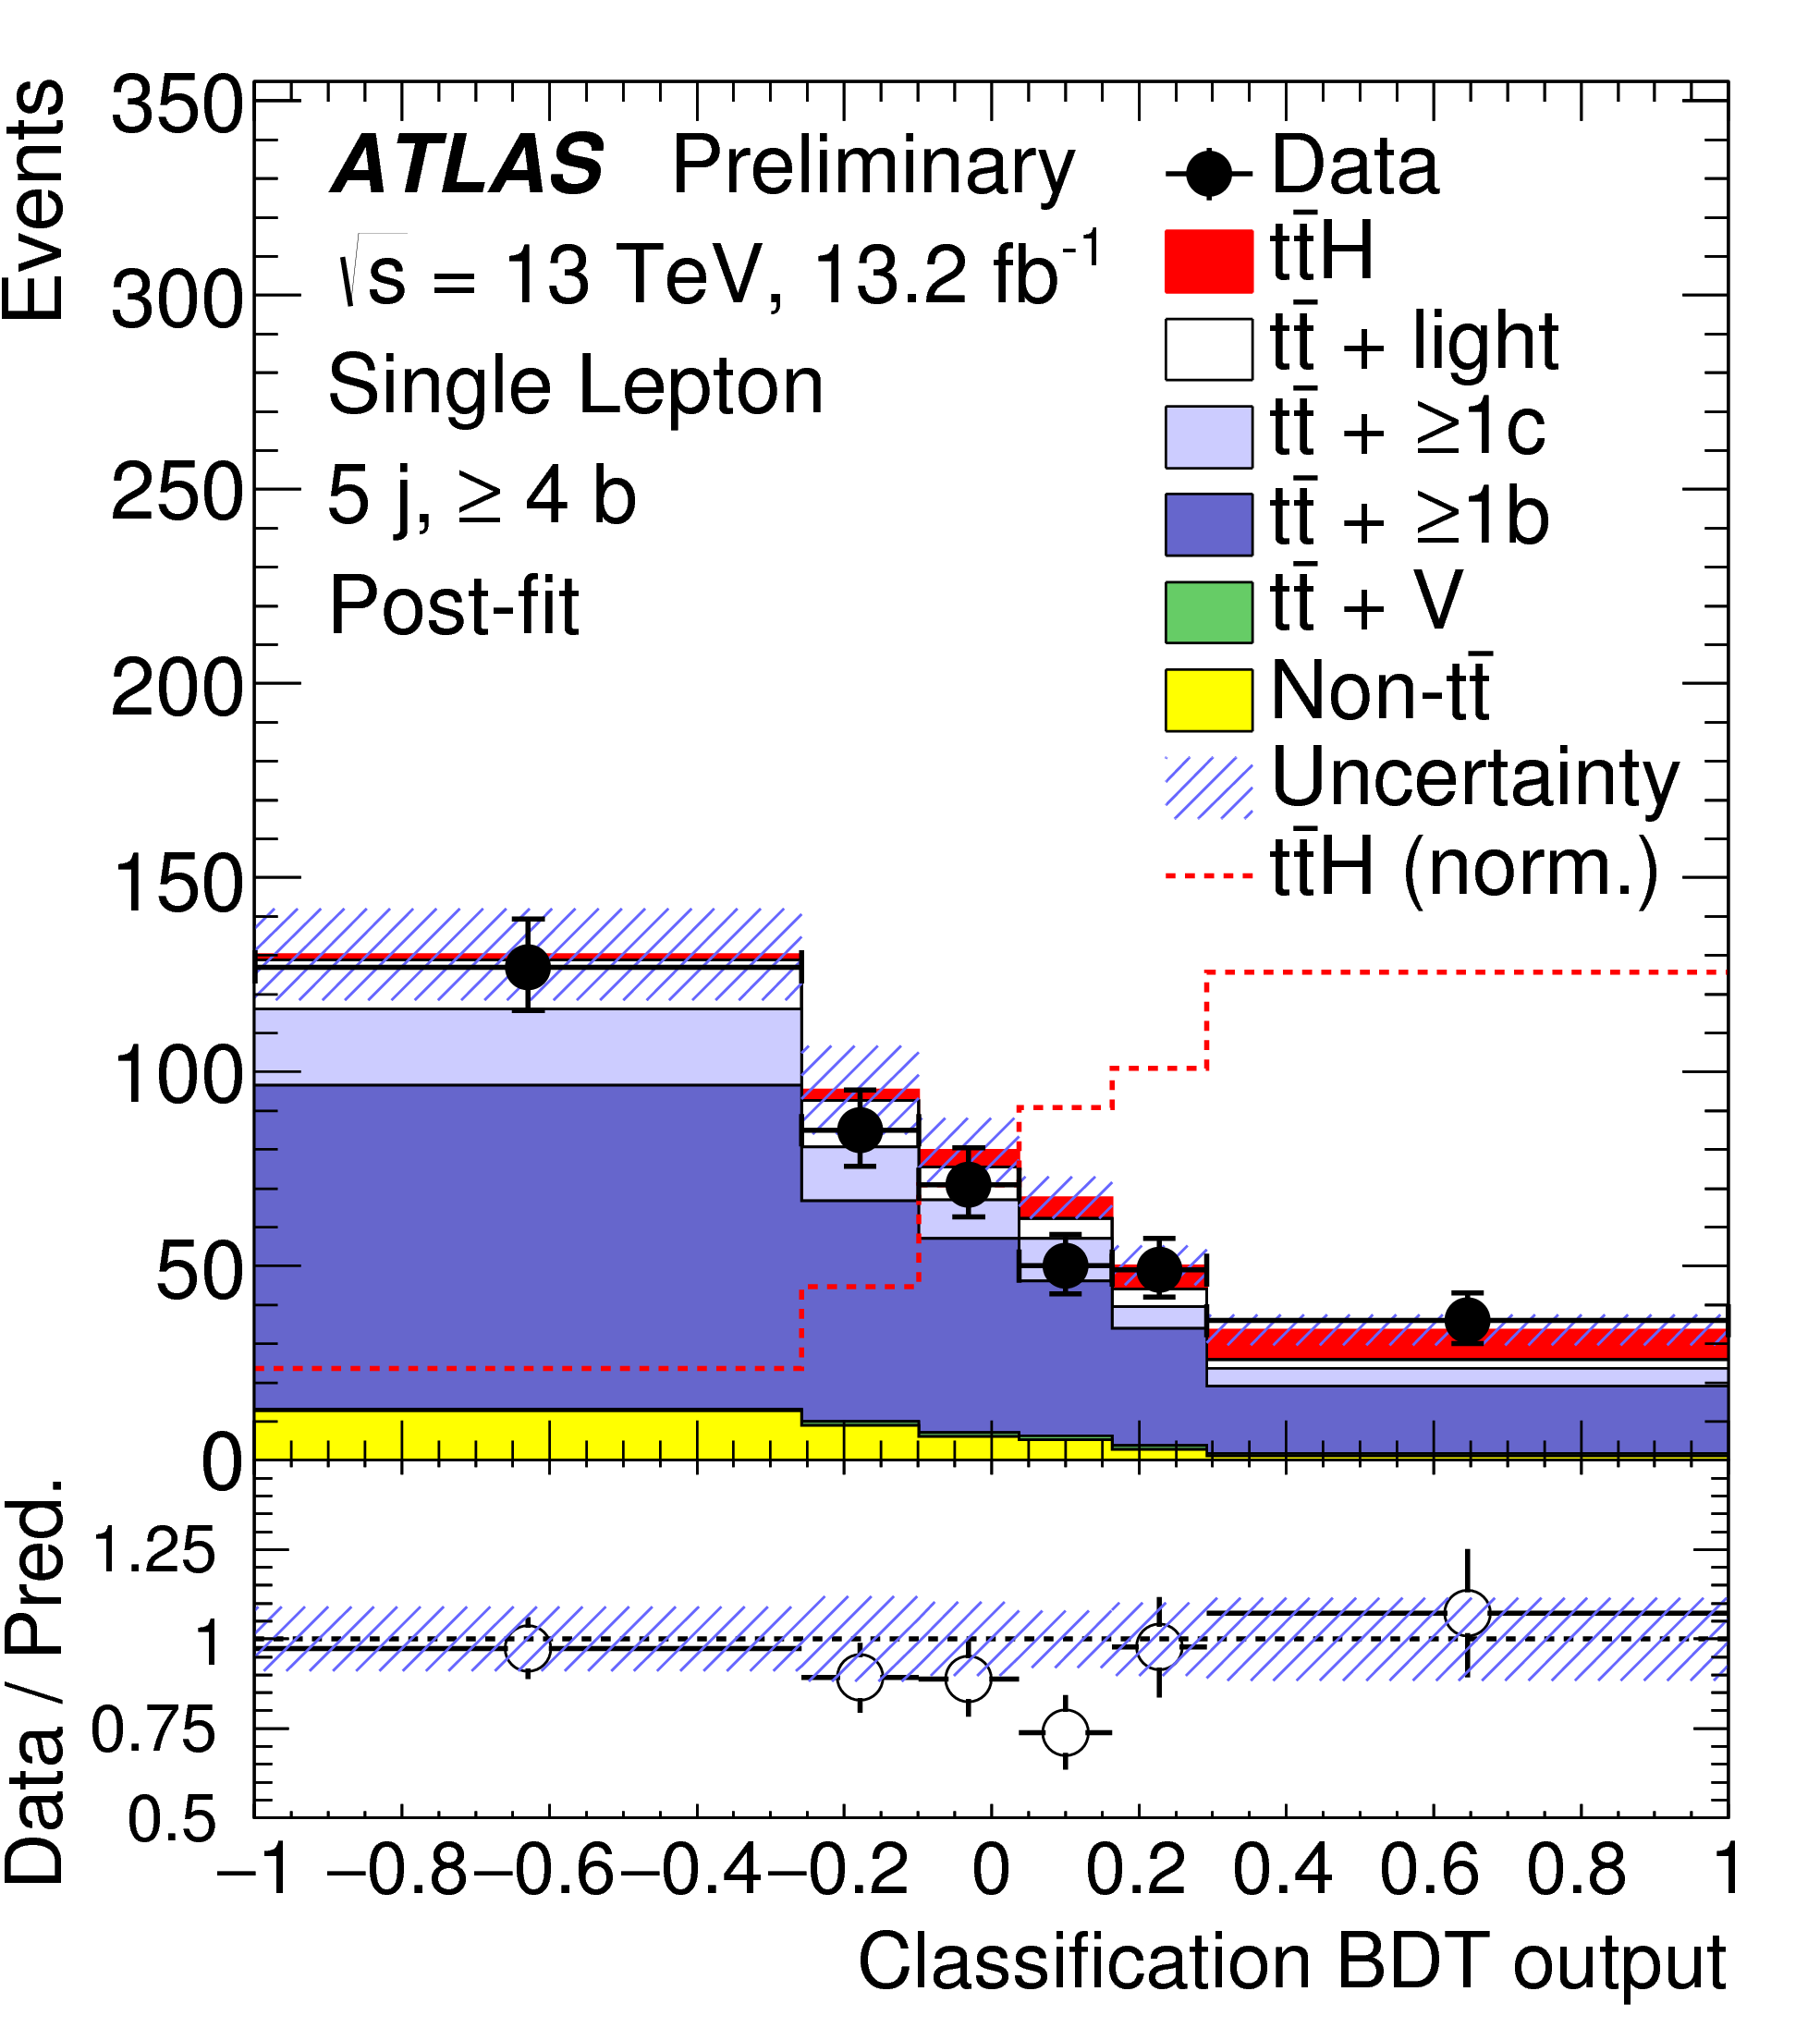
\includegraphics[width=0.9\textwidth]{figures/ttH/fig_11b.png}
  \caption{}
  \label{}
\end{subfigure}
\begin{subfigure}{0.24\textwidth}
  \centering
  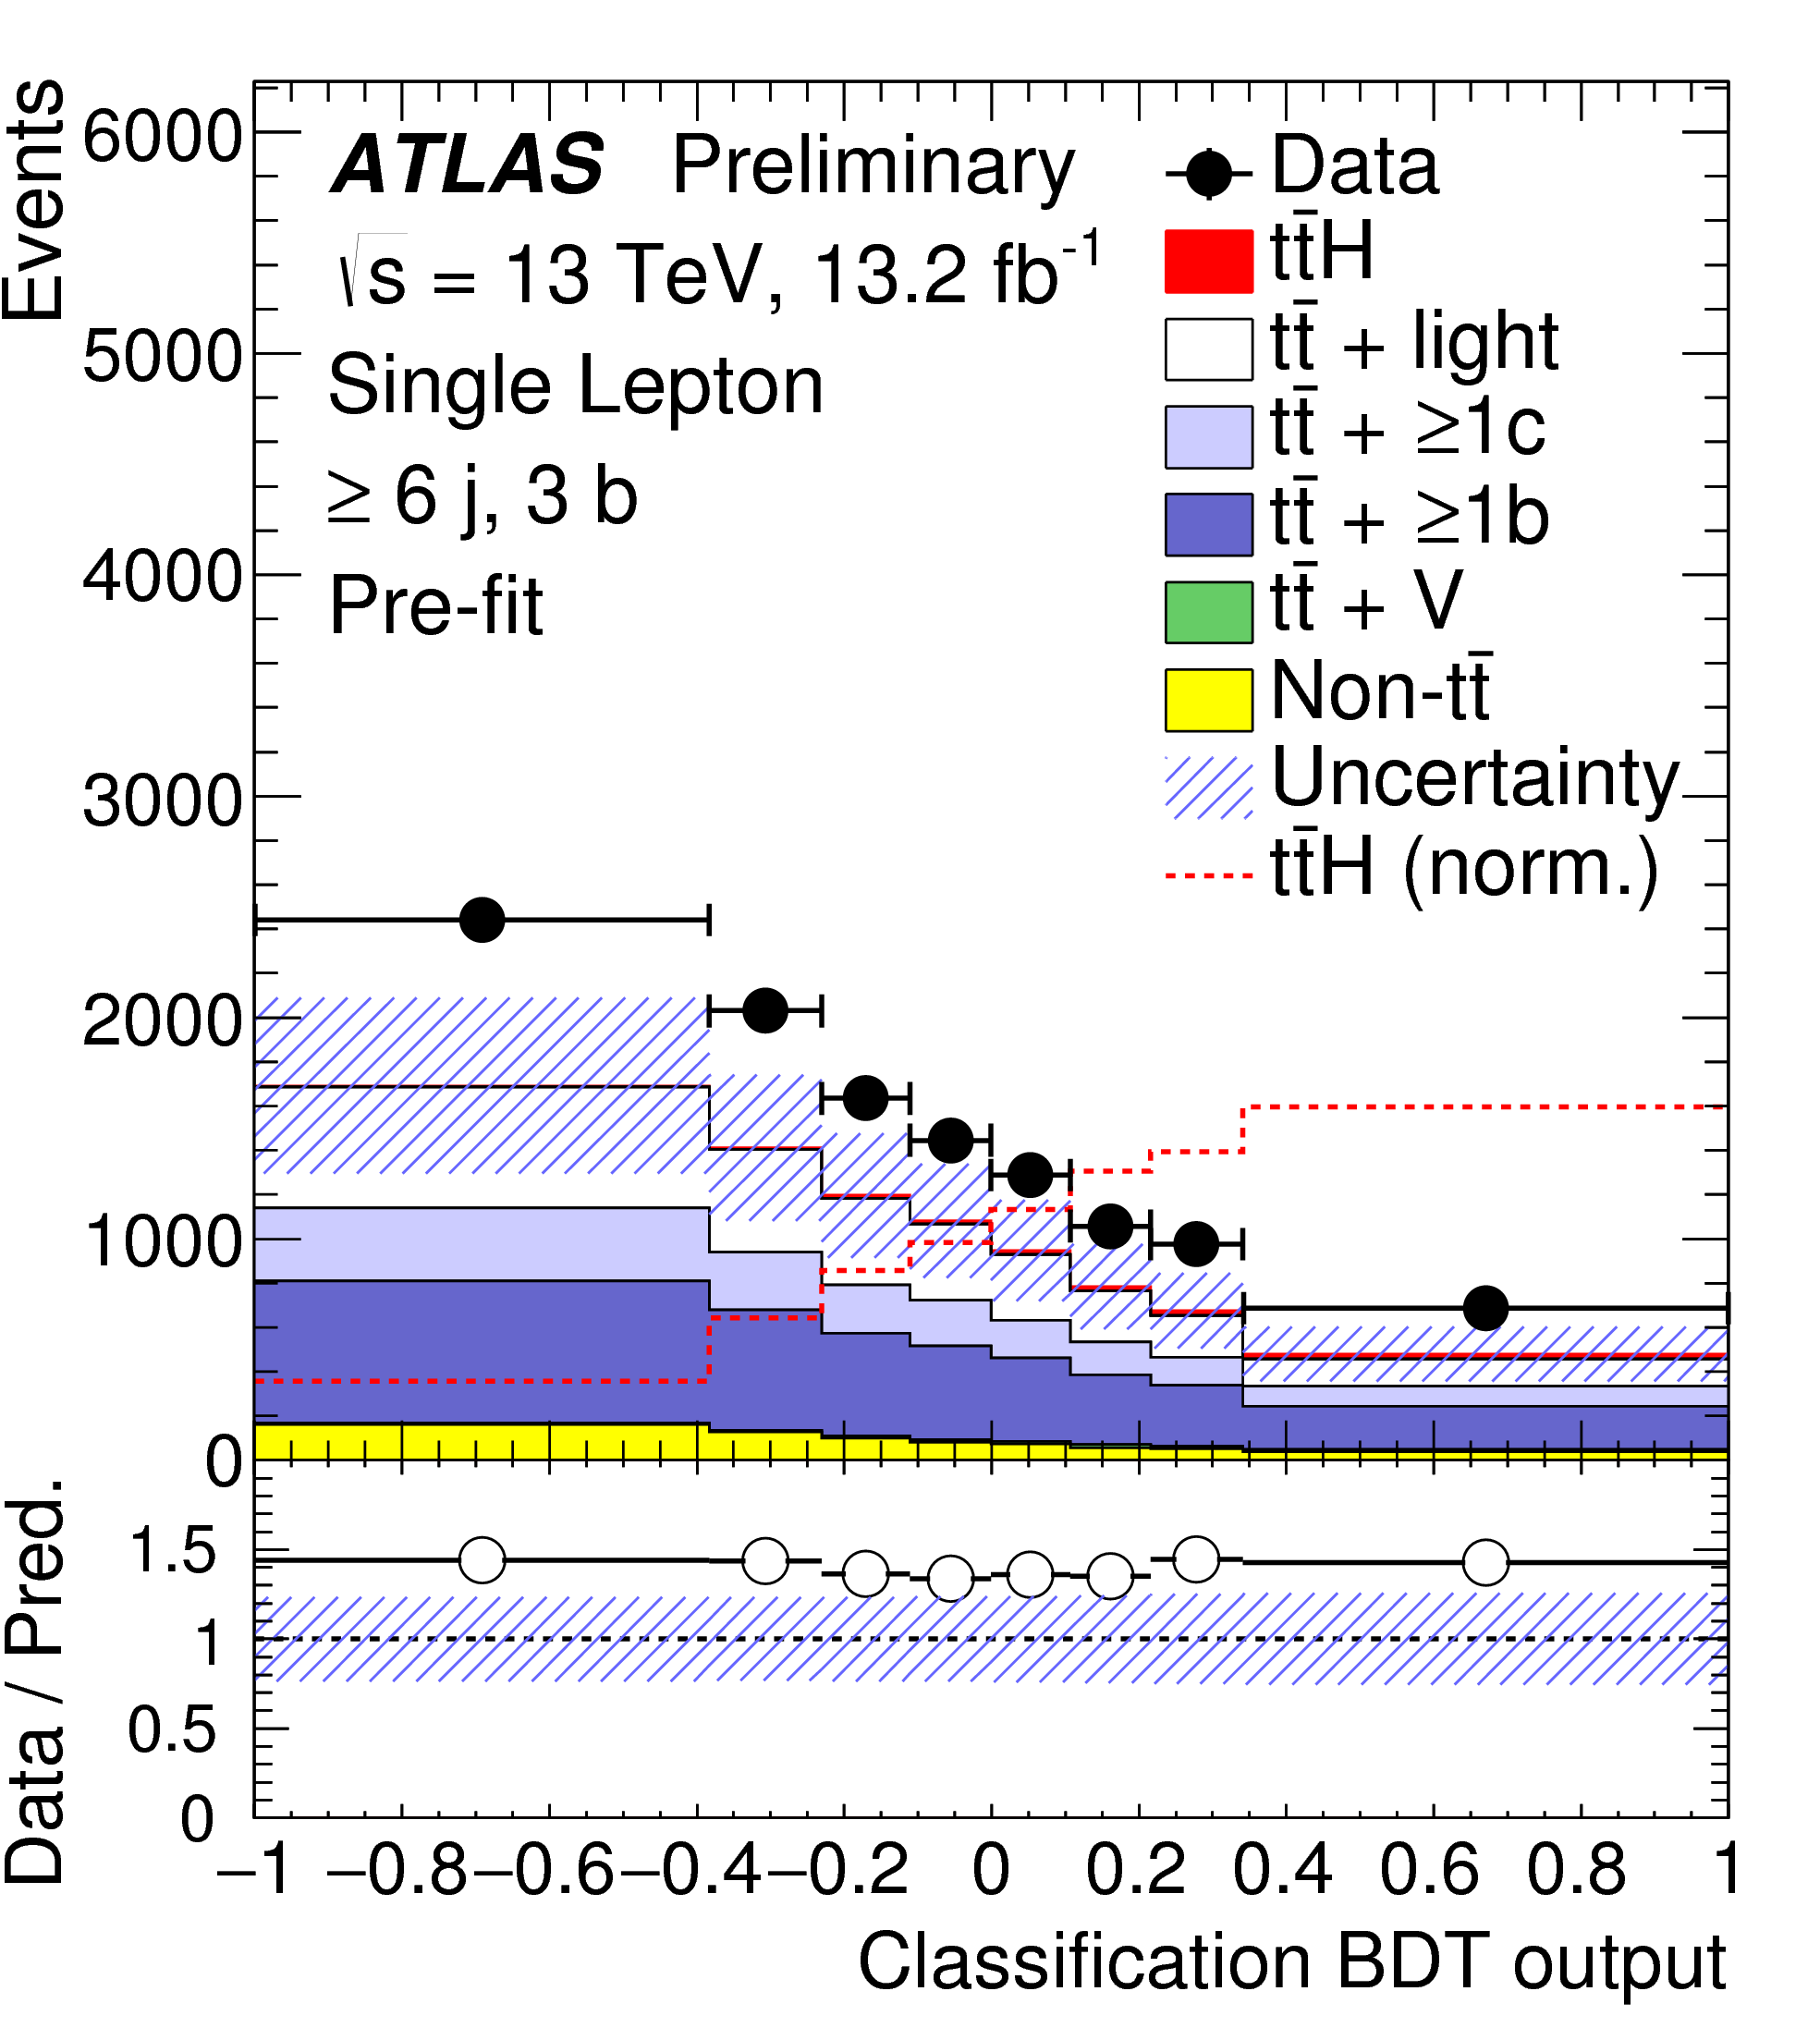
\includegraphics[width=0.9\textwidth]{figures/ttH/fig_11c.png}
  \caption{}
  \label{}
\end{subfigure}
\begin{subfigure}{0.24\textwidth}
  \centering
  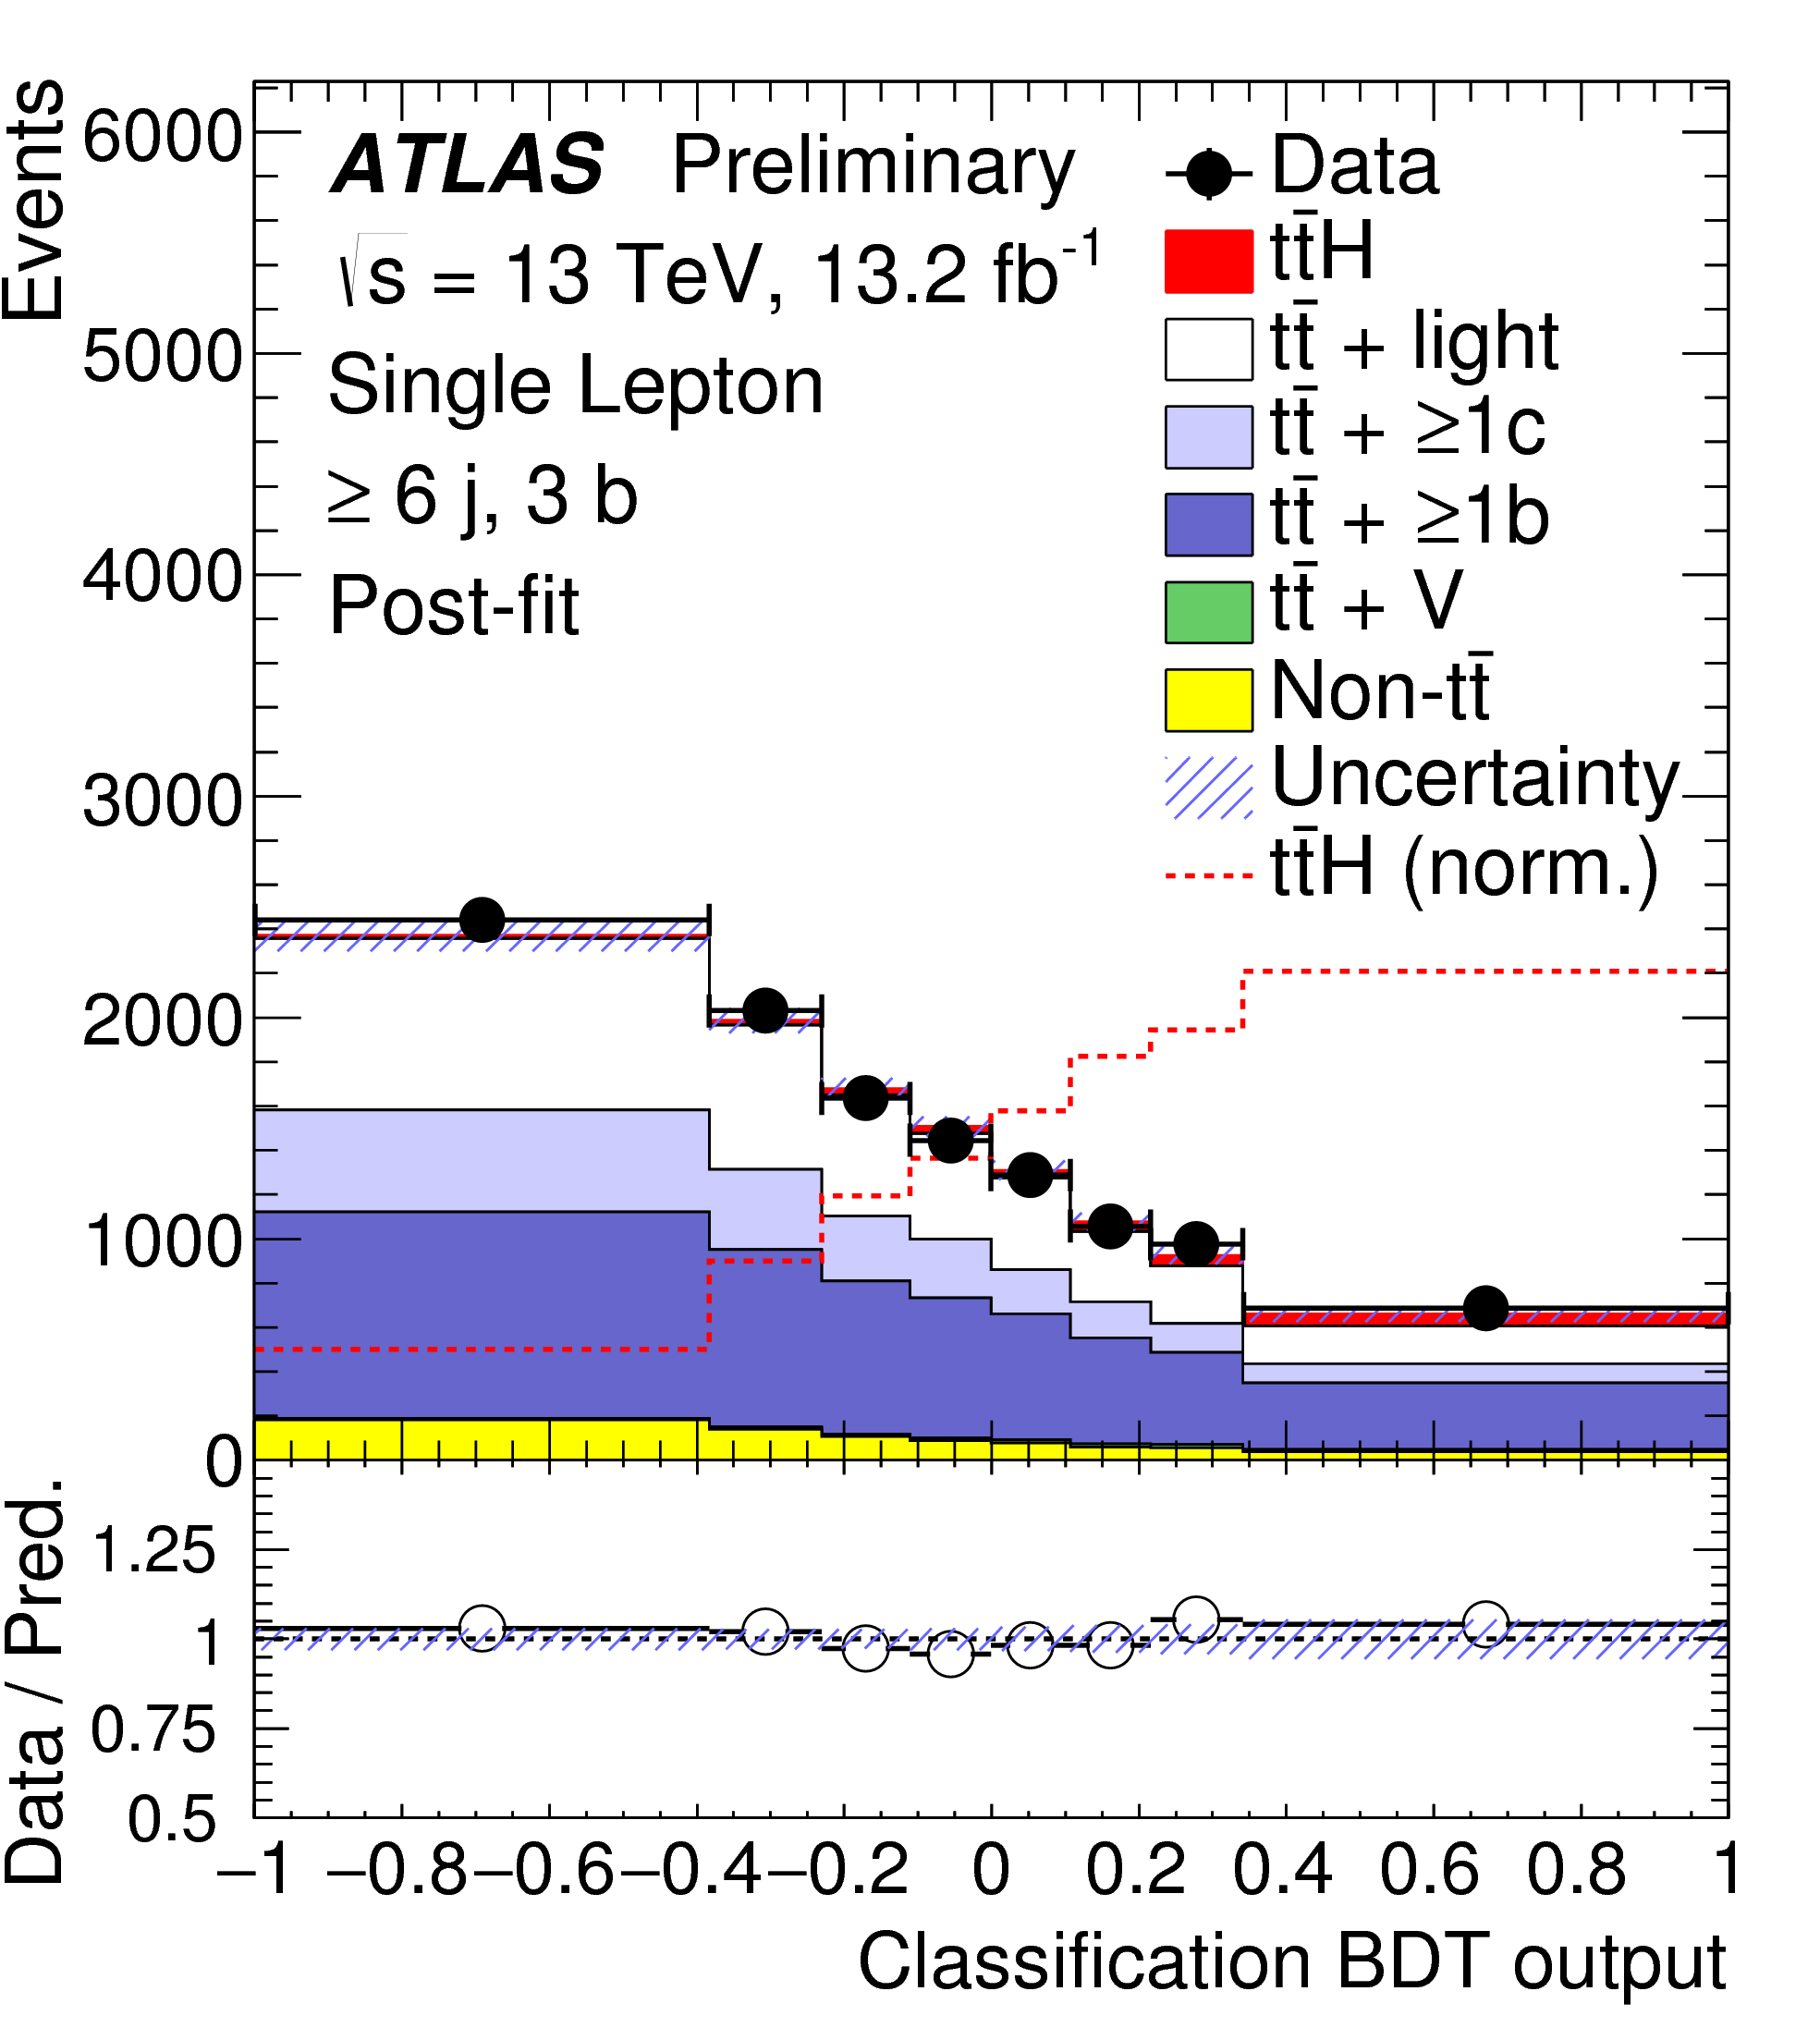
\includegraphics[width=0.9\textwidth]{figures/ttH/fig_11d.png}
  \caption{}
  \label{}
\end{subfigure}
\begin{center}
\begin{subfigure}{0.24\textwidth}
  \centering
  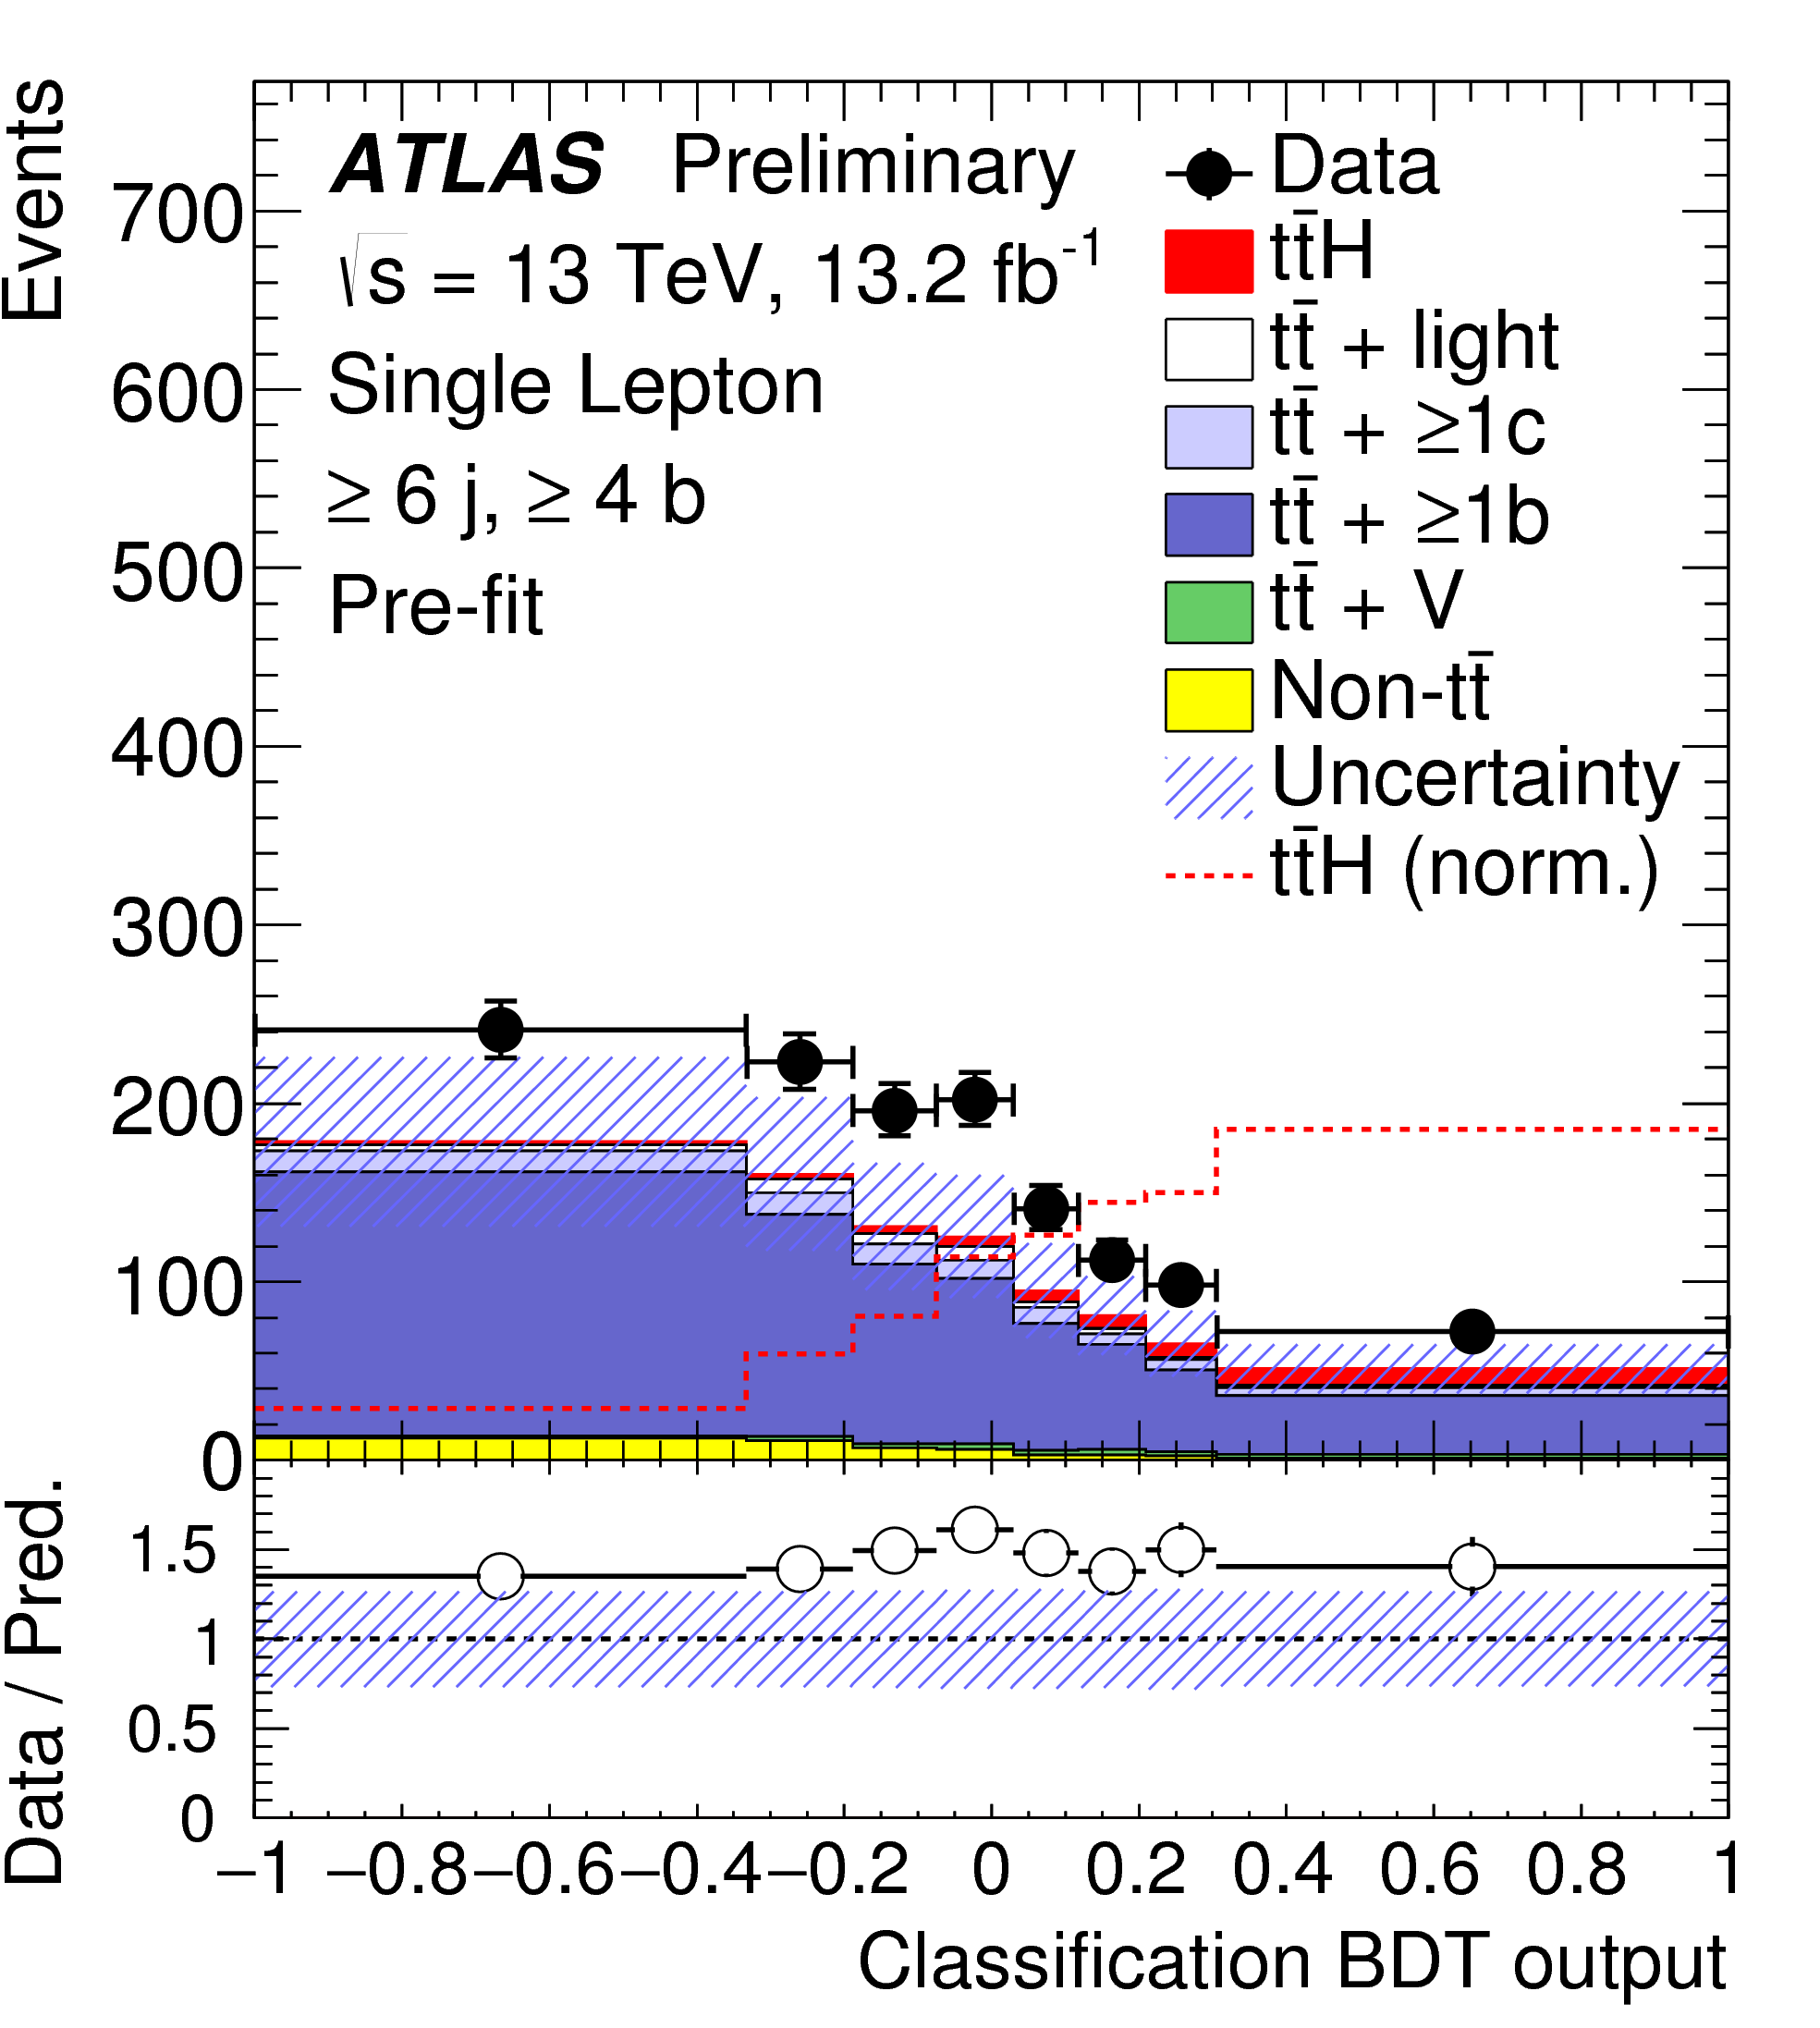
\includegraphics[width=0.9\textwidth]{figures/ttH/fig_11e.png}
  \caption{}
  \label{}
\end{subfigure}
\begin{subfigure}{0.24\textwidth}
  \centering
  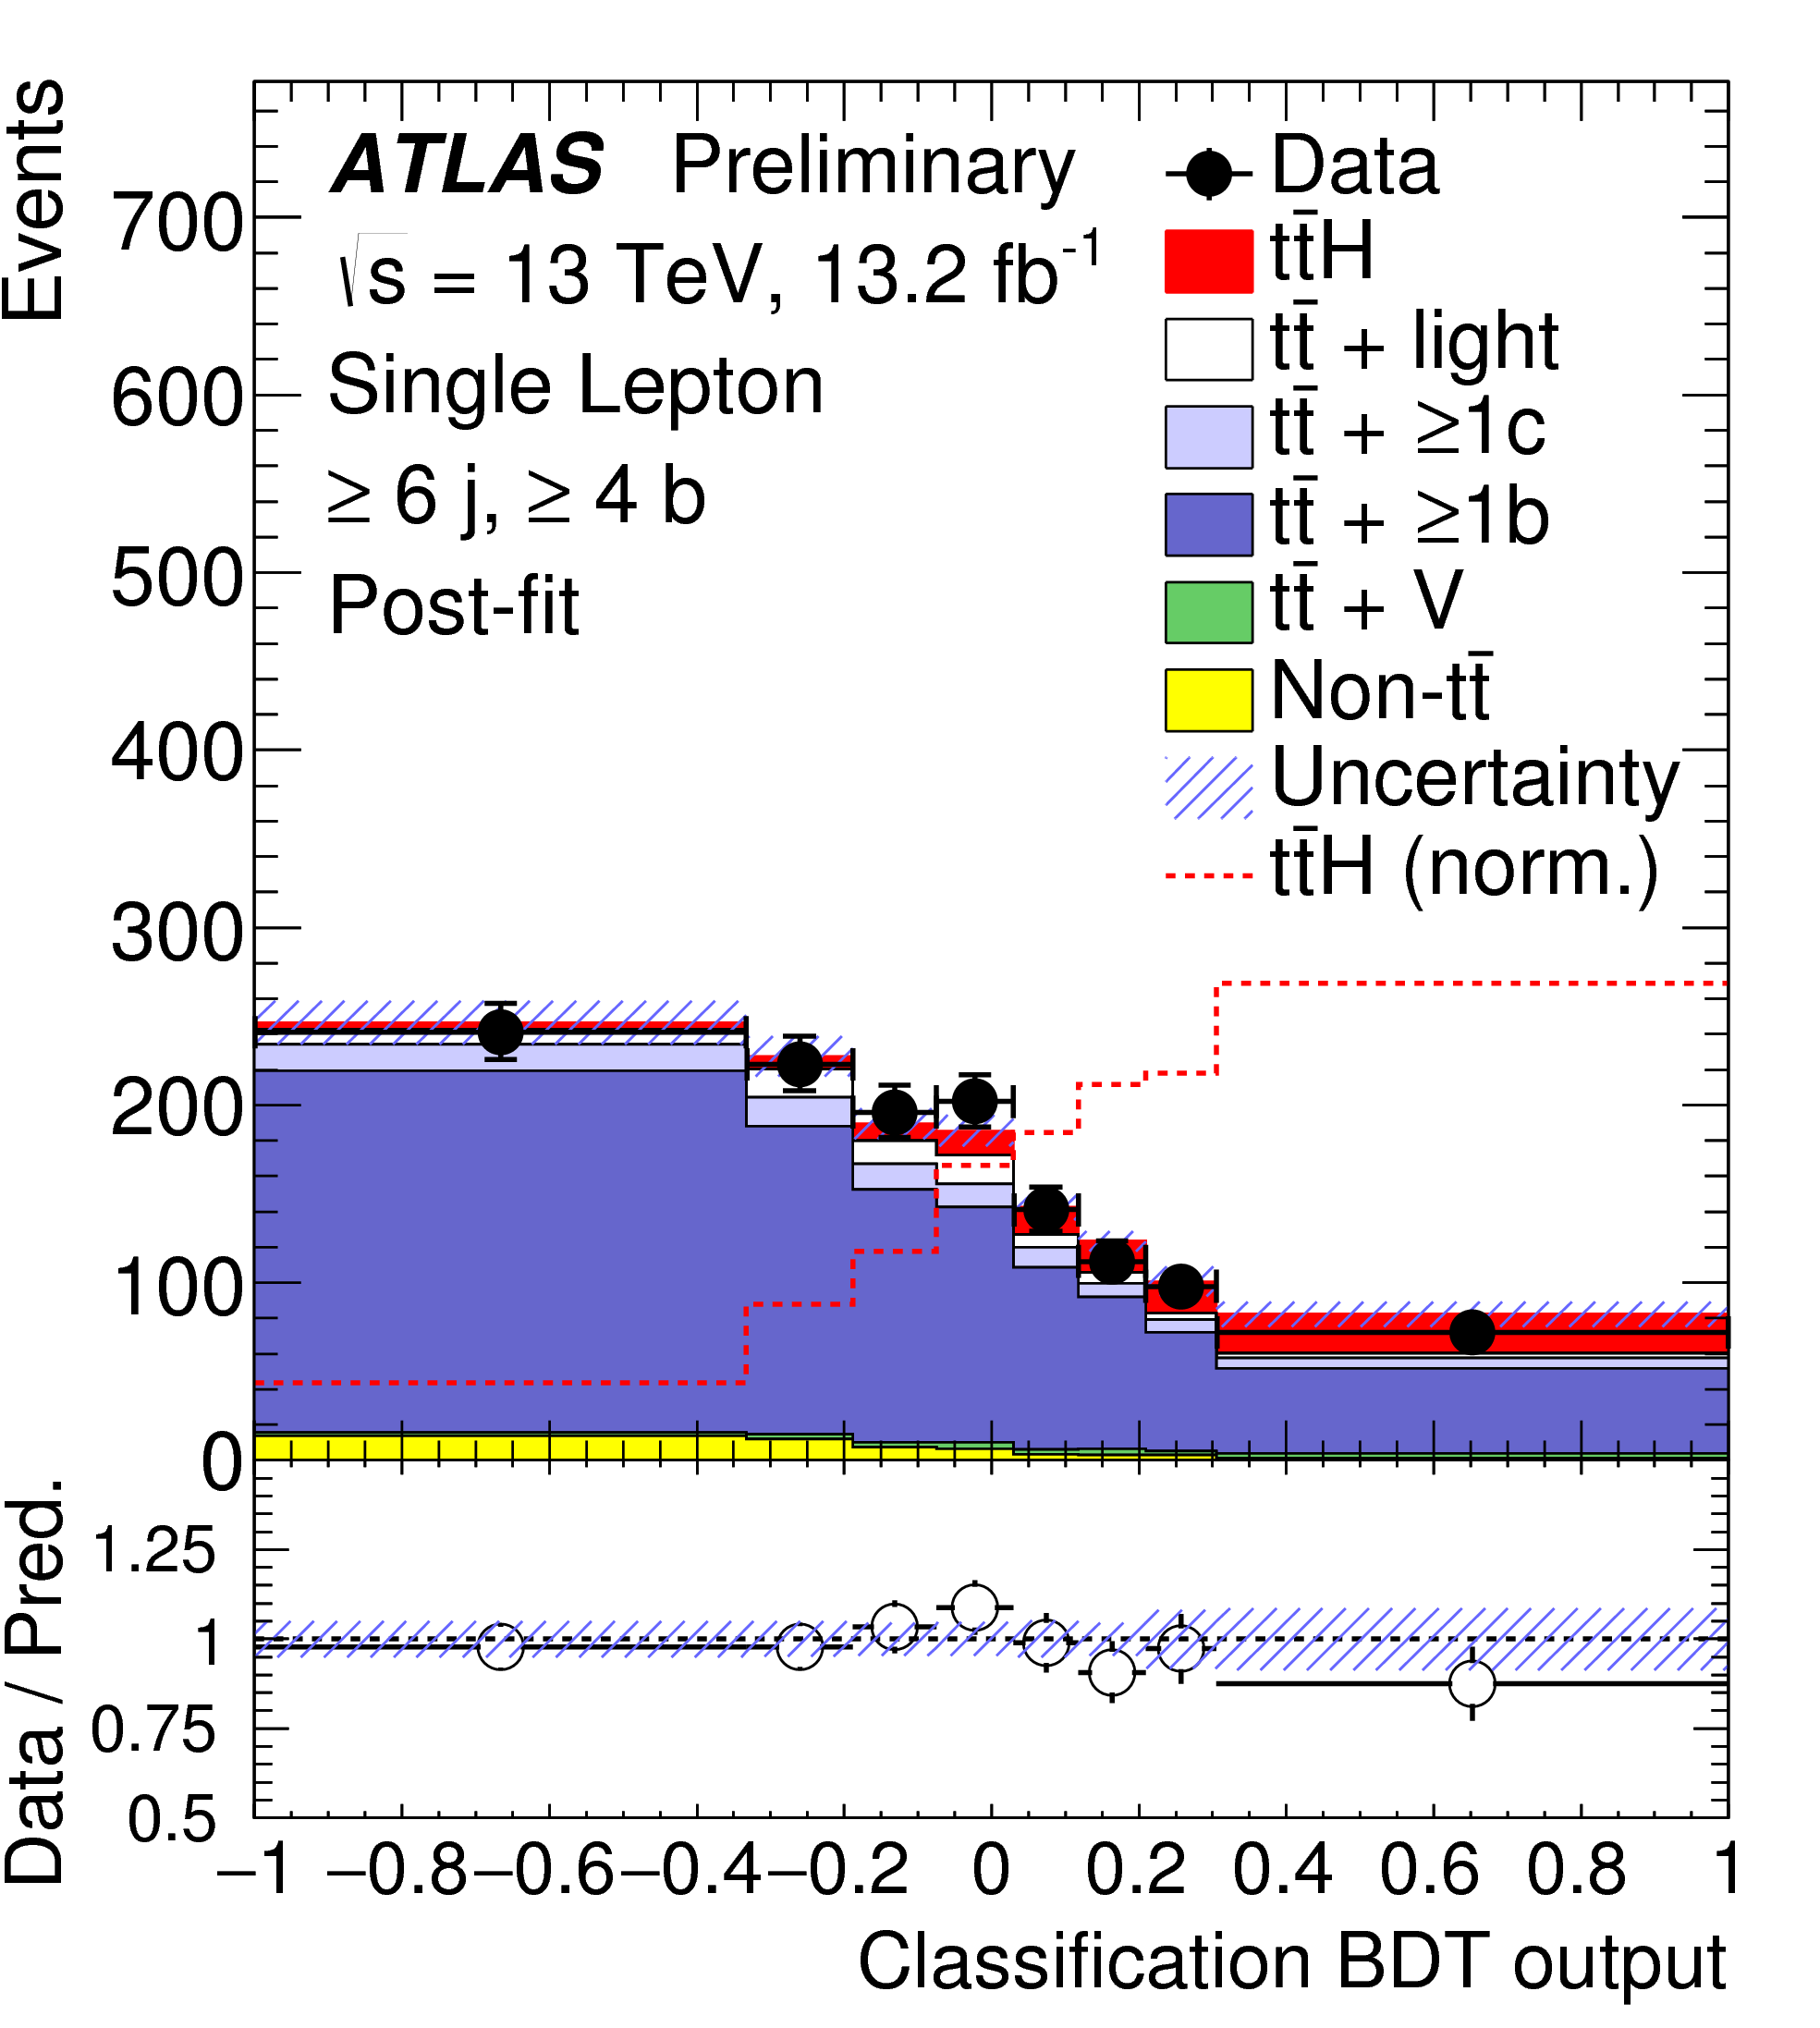
\includegraphics[width=0.9\textwidth]{figures/ttH/fig_11f.png}
  \caption{}
  \label{}
\end{subfigure}
\end{center}


\captionsetup{width=0.85\textwidth}  \caption{\small Comparison between the data and prediction for the classification BDT output distributions before and after performing the combined fit to data in the single-lepton and dilepton channels (``Pre-fit'' and ``Post-fit'', respectively) under the signal-plus-background hypothesis. Shown are the (5j,$\ge$4b) region (a) pre-fit and (b) post-fit, the ($\ge$6j, 3b) region (c) pre-fit and (d) post-fit, and the (6j, $\ge$4b) region (e) pre-fit and (f) post-fit.
The small contributions from single top, $W/Z$+jets, diboson, and multijet backgrounds are combined into a single background source  referred to as ``Non-$t\bar{t}$''. The last bin in all figures contains the overflow. The bottom panels display the ratios of data to the total background prediction (``Bkg''). The blue triangles indicate points that are outside the vertical range of the figure. The hashed area represents the total uncertainty on the background. In the case of the pre-fit background uncertainty, the normalisation uncertainties on the $t\bar{t}+\ge1b$ and $t\bar{t}+\ge1c$ backgrounds are not included.}
\label{sec:tth:fig:bdt}
\end{figure}


\begin{figure}[htbp!]
\begin{subfigure}{0.5\textwidth}
  \centering
  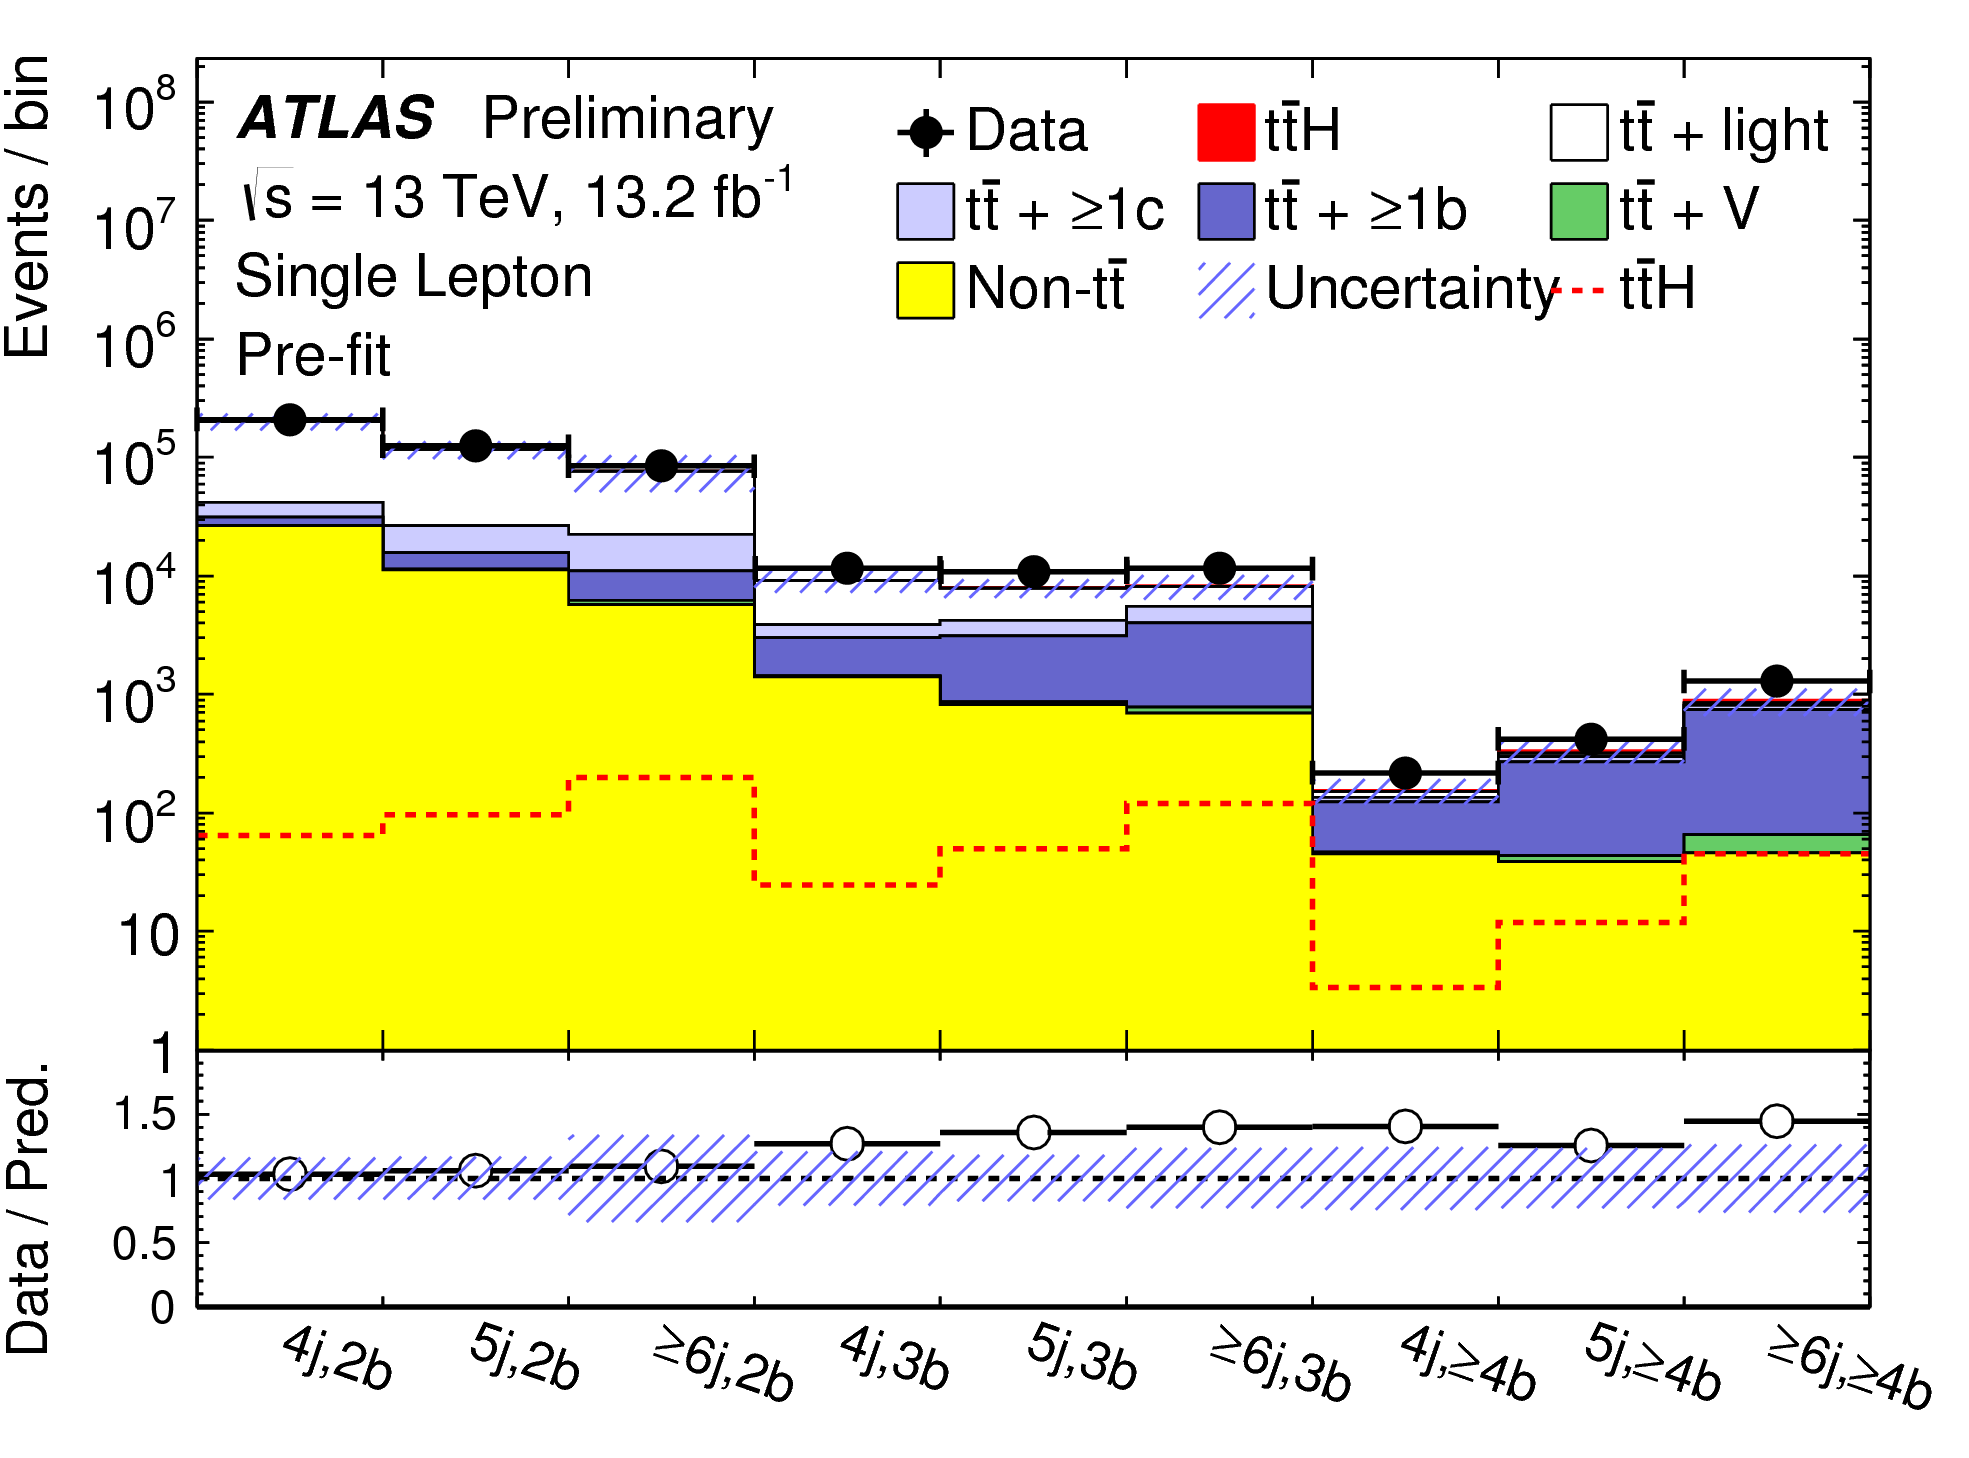
\includegraphics[width=0.9\textwidth]{figures/ttH/fig_04b.png}
  \caption{}
  \label{}
\end{subfigure}
\begin{subfigure}{0.5\textwidth}
  \centering
  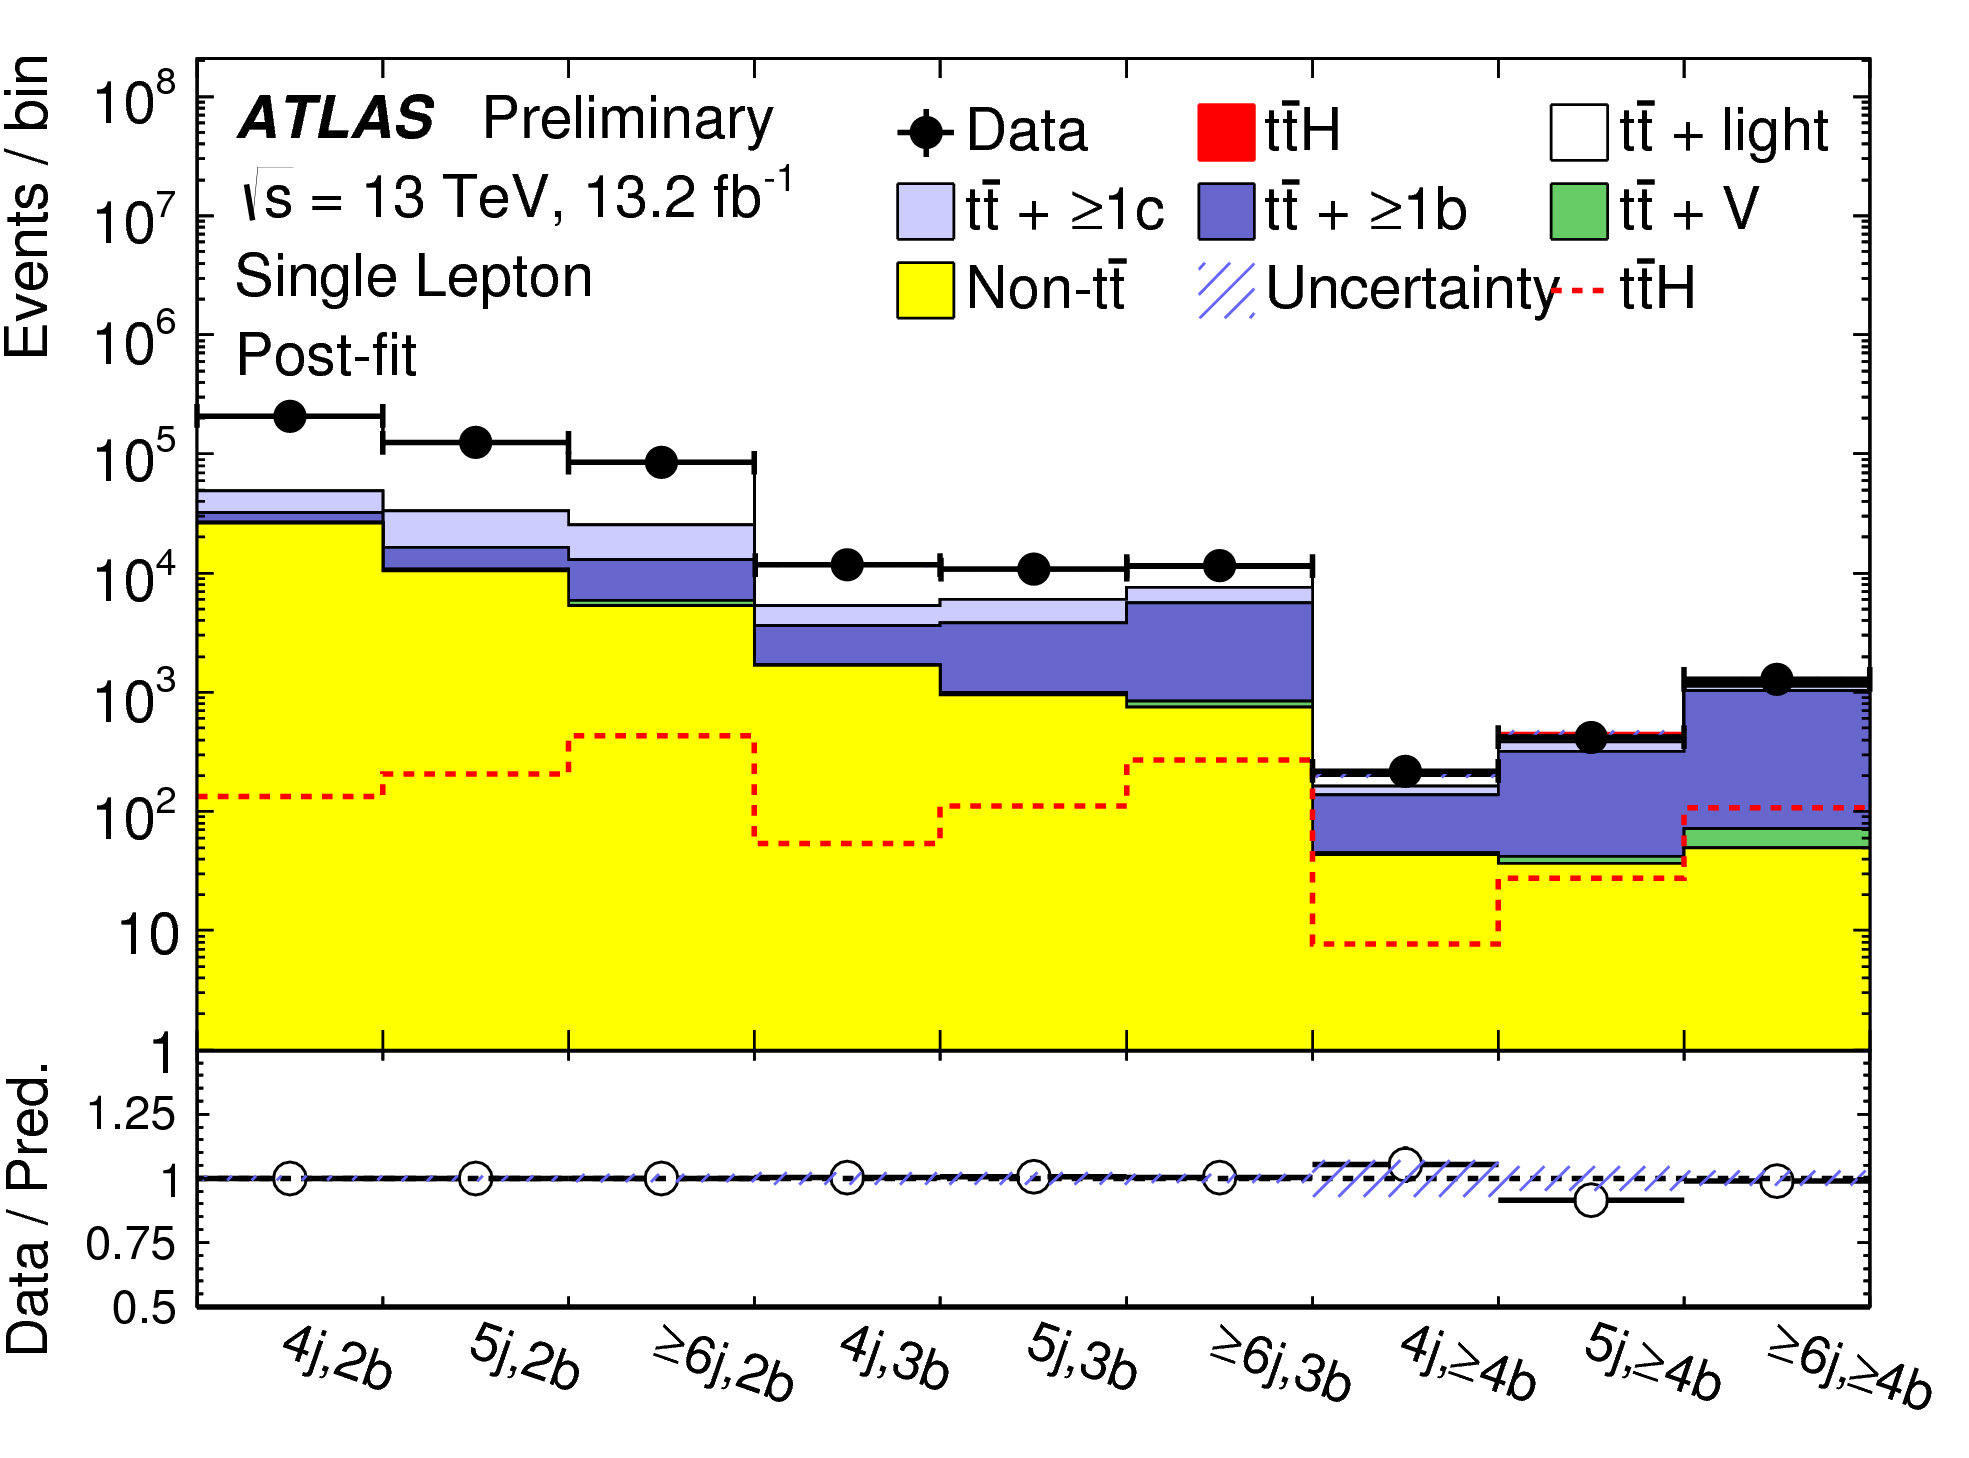
\includegraphics[width=0.9\textwidth]{figures/ttH/fig_17b.png}
  \caption{}
  \label{}
\end{subfigure}
\captionsetup{width=0.85\textwidth}  \caption{\small Comparison between the data and background prediction for the yields in each of the search regions considered (a) before the fit (``Pre-fit'') and (b) after the fit (``Post-fit''). The fit is performed on the data in single-lepton and dilepton channels under the signal-plus-background hypothesis. The small contributions from single top, $W/Z$+jets, diboson, and multijet backgrounds are combined into a single background source  referred to as ``Non-$t\bar{t}$''. The last bin in all figures contains the overflow. The bottom panels display the ratios of data to the total background prediction (``Bkg''). The blue triangles indicate points that are outside the vertical range of the figure. The hashed area represents the total uncertainty on the background. In the case of the pre-fit background uncertainty, the normalisation uncertainties on the $t\bar{t}+\ge1b$ and $t\bar{t}+\ge1c$ backgrounds are not included.}
\label{sec:ttH:fig:summary}
\end{figure}

\begin{table}[htbp]
  \centering
  \begin{footnotesize}{
  \begin{tabular}{|l ||  r@{$~\pm~$}l |  r@{$~\pm~$}l ||  r@{$~\pm~$}l  | r@{$~\pm~$}l || r@{$~\pm~$}l | r@{$~\pm~$}l |}
    \hline
    & \multicolumn{4}{c||}{4j, 2b} & \multicolumn{4}{c||}{4j, 3b} & \multicolumn{4}{c|}{4j, $\ge$4b} \\
    & \multicolumn{2}{c|}{Pre-fit} & \multicolumn{2}{c||}{Post-fit} & \multicolumn{2}{c|}{Pre-fit} & \multicolumn{2}{c||}{Post-fit} & \multicolumn{2}{c|}{Pre-fit} & \multicolumn{2}{c|}{Post-fit} \\
    \hline
    $t\bar{t}$ + light-jets & 160000&30000 &  158800&4800  & 5300&1500 &  6300&440  & 17&11 &  36&14  \\
    $t\bar{t}+\ge1c$   & 10800&2400 & 16800&4100  & 880&300  &  1680&350 & 11.7&5.4  &  24.4&6.3  \\
    $t\bar{t}+\ge1b$   & 4580&930   &  5760&980   & 1570&470 &  1930&320 & 76&24     &  94&13  \\
    $t\bar{t}$+V & 212&27     &  218&24     & 18.4&3.8 &  20.4&3.6 & 1.60&0.42 &  1.73&0.33  \\
    Single top & 10300&1700 &  10400&1300 & 390&87   &  476&80   & 9.6&3.5   &  12.9&3.2  \\
    $W/Z$+jets & 6500&2400  &  7800&2200  & 220&100  &  410&150  & 2.1&1.2   &  2.6&1.2  \\
    Diboson    & 420&220    &  390&190    & 15&10    &  19&11    & 3.9&3.3   &  3.5&3.0  \\
    Multijet & 9200&4200  &  7800&1500  & 770&360  &  770&240  & 29&27     &  23&23  \\
    $tH$       &  9.3&1.3   &   9.3&1.2   & 4.41&0.66&   4.55&0.57  & 0.62&0.13  & 0.64&0.10  \\
    \hline
%     Total background  & 201557&32429.6 & 208026&1877.62 & 9165.79&1918.68 & 11608.3&297.137 & 152.009&44.3394 & 199.347&28.2757 \\
    Total background  & 202000&32000 &  208000&1900  & 9200&1900 &  11610&300  & 152&44 &  199&28 \\
    \hline
    $t\bar{t}H$     & 63.8&6.2   &   134&42    & 24.6&4.1 &   54&21   & 3.32&0.87 &   7.7&2.9  \\
    \hline
    Total             & 202000&32000 &  208200&1900  & 9200&1900 &  11660&300  & 155&45 &  207&28  \\
    \hline
    Data & \multicolumn{4}{c||}{208239} & \multicolumn{4}{c||}{11686} & \multicolumn{4}{c|}{218} \\
    \hline 
    \multicolumn {13}{|c|}{}\\
    \hline
    & \multicolumn{4}{c||}{5j, 2b} & \multicolumn{4}{c||}{5j, 3b} & \multicolumn{4}{c|}{5j, $\ge$4b} \\
    & \multicolumn{2}{c|}{Pre-fit} & \multicolumn{2}{c||}{Post-fit} & \multicolumn{2}{c|}{Pre-fit} & \multicolumn{2}{c||}{Post-fit} & \multicolumn{2}{c|}{Pre-fit} & \multicolumn{2}{c|}{Post-fit} \\
    \hline
    $t\bar{t}$ + light-jets & 91000&17000 &  91500&3900  & 3640&880 &  4580&450  & 24&15 &  45&19  \\
    $t\bar{t}+\ge1c$   & 10800&2100 &  16600&3800 & 1170&330  &  2150&410  & 30&12     &  64&11  \\
    $t\bar{t}+\ge1b$   & 4440&530   &  5760&840   & 2230&460  &  2830&370  & 224&62    &  278&29  \\
    $t\bar{t}$+V & 277&33     &  287&30     & 35.3&6.1  &  39.6&5.9  & 4.9&1.5   &  5.4&1.4  \\
    Single top & 4900&1200  &  4790&690   & 305&87    &  338&67    & 14.3&5.6  &  16.1&3.9  \\
    $W/Z$+jets & 2700&1100  &  2720&780   & 200&100   &  300&120   & 3.0&3.0   &  3.3&2.3  \\
    Diboson    & 200&110    &  210&110    & 15.7&9.7  &  16.0&8.7  & 0.39&0.28 &  0.43&0.29  \\
    Multijet & 3300&1500  &  2800&670   & 300&150   &  300&110   & 20&17     &  16&16  \\
    $tH$       & 7.4&1.3    &   7.5&1.3   & 3.88&0.72 &  4.14&0.69 & 0.82&0.16 &  0.91&0.14   \\
    \hline
%     Total background  & 117409&19524.8 & 124656&1404.37 & 7890.7&1423.65 & 10561.1&280.972 & 321.518&78.0279 & 429.318&27.8377 \\
    Total background & 117000&20000 &  124600&1400 &  7900&1400 &  10560&280  & 322&78 &  429&28 \\
    \hline
    $t\bar{t}H$     & 96.5&7.7   &   206&61    & 49.7&6.9  &   110&42   & 11.8&2.6  &    27&10   \\
    \hline
    Total            & 118000&20000 &  124900&1400 &  7900&1400 &  10670&280  & 333&79 &  457&27  \\
    \hline
    Data & \multicolumn{4}{c||}{124688} & \multicolumn{4}{c||}{10755} & \multicolumn{4}{c|}{418} \\
    \hline 
    \multicolumn {13}{|c|}{}\\
    \hline
    & \multicolumn{4}{c||}{$\ge$6j, 2b} & \multicolumn{4}{c||}{$\ge$6j, 3b} & \multicolumn{4}{c|}{$\ge$6j, $\ge$4b} \\
    & \multicolumn{2}{c|}{Pre-fit} & \multicolumn{2}{c||}{Post-fit} & \multicolumn{2}{c|}{Pre-fit} & \multicolumn{2}{c||}{Post-fit} & \multicolumn{2}{c|}{Pre-fit} & \multicolumn{2}{c|}{Post-fit} \\
    \hline
    $t\bar{t}$ + light-jets & 54000&24000 &  58600&4000  & 2600&1100 &  3610&500  & 34&22 & 74&32 \\
    $t\bar{t}+\ge1c$   & 11500&3700  &  12500&5200 & 1550&560 &  1960&660 & 71&37     &  91&36  \\
    $t\bar{t}+\ge1b$   & 4800&1200   &  7180&920   & 3240&800 &  4830&470 & 670&190   &  955&70  \\
    $t\bar{t}$+V & 470&61      &  498&49     & 86&13    &  98&10    & 19.1&4.2  &  22.3&3.5  \\
    Single top & 2690&840    &  2430&400   & 278&100  &  286&65   & 29&14     &  32&12  \\
    $W/Z$+jets & 1610&660    &  1720&520   & 121&55   &  169&65   & 11.9&6.7  &  12.9&6.4  \\
    Diboson    & 164&88      & 166&83      & 14.4&8.3 & 15.8&8.4  & 2.0&1.3   & 2.1&1.3 \\
    Multijet & 1220&560    & 1050&310    & 270&150  & 270&120   & 1.2&1.2   & 1.2&1.2 \\
    $tH$       & 9.6&2.4     &  9.9&2.3    &  5.7&1.5 &  6.2&1.5  & 1.86&0.53 & 2.10&0.50  \\
    \hline
%     Total background  & 76899.6&26163.8 & 84203.6&1355.39 & 8150.26&1925.91 & 11248&237.559 & 843.633&226.43 & 1191.34&55.3123 \\
    Total background & 77000&26000 &  84200&1400  & 8200&1900 &  11250&240  & 840&230 & 1191&55 \\
    \hline
    $t\bar{t}H$     & 198&18      &   430&120   & 119&16   &   261&99  & 44.9&9.4  &    107&39   \\
    \hline
    Total            & 77000&26000 &  84600&1400  & 8300&1900 &  11520&220  & 890&230 & 1298&41 \\
    \hline
    Data & \multicolumn{4}{c||}{84556} & \multicolumn{4}{c||}{11561} & \multicolumn{4}{c|}{1285} \\
    \hline
  \end{tabular}
  }\end{footnotesize}
 \captionsetup{width=0.85\textwidth}  \caption{\small Expected and observed event yields in the single lepton channel. Post-fit yields are after the combined fit to data in the single-lepton and dilepton channels under the signal-plus-background hypothesis.
  The quoted uncertainties are the sum in quadrature of statistical and systematic uncertainties on the yields. In the pre-fit case, they do not include the uncertainties on the $t\bar{t} + \ge1b$ or $t\bar{t} + \ge1c$ normalisations. In the post-fit case, these uncertainties are computed taking into account correlations among nuisance parameters and among processes, including the uncertainties on the determination of the $t\bar{t} + \ge1b$ and $t\bar{t} + \ge1c$ normalisations.  For the $t\bar{t}H$ signal, the pre-fit yield values correspond to the theoretical prediction and corresponding uncertainties, whilst the post-fit yields and uncertainties correspond to those on the signal strength measurement.
  }
  \label{tab:tth:SLyields}
\end{table}


